% Auto-generated by cmd/render — the contrast map as a TikZ figure.
% One grid per Kind over the scored scenarios. Orange = signal (verdict
% from fdr.gen.tex), grey = measured, no marginal signal (deeper grey =
% higher raw saliency, i.e. destabilization), dashed outline = negative
% control (defines the fragility floor), dark cell with * = deciding locus
% (the injected fault, never scored).
% \input-able fragment; requires \usepackage{tikz}.

\par\medskip\noindent{\small\bfseries ConfigMap}\par\smallskip
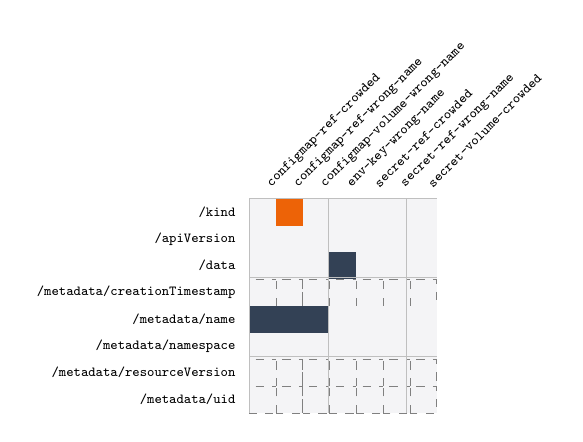
\begin{tikzpicture}[x=3.4mm,y=3.4mm]
\node[rotate=45,anchor=west,font=\ttfamily\tiny] at (0.5,0.25) {configmap-ref-crowded};
\node[rotate=45,anchor=west,font=\ttfamily\tiny] at (1.5,0.25) {configmap-ref-wrong-name};
\node[rotate=45,anchor=west,font=\ttfamily\tiny] at (2.5,0.25) {configmap-volume-wrong-name};
\node[rotate=45,anchor=west,font=\ttfamily\tiny] at (3.5,0.25) {env-key-wrong-name};
\node[rotate=45,anchor=west,font=\ttfamily\tiny] at (4.5,0.25) {secret-ref-crowded};
\node[rotate=45,anchor=west,font=\ttfamily\tiny] at (5.5,0.25) {secret-ref-wrong-name};
\node[rotate=45,anchor=west,font=\ttfamily\tiny] at (6.5,0.25) {secret-volume-crowded};
\node[anchor=east,font=\ttfamily\tiny] at (-0.15,-0.5) {/kind};
\fill[fill={rgb,255:red,244;green,244;blue,246}] (0,-1) rectangle ++(1,1);
\fill[fill={rgb,255:red,237;green,99;blue,7}] (1,-1) rectangle ++(1,1);
\fill[fill={rgb,255:red,244;green,244;blue,246}] (2,-1) rectangle ++(1,1);
\fill[fill={rgb,255:red,244;green,244;blue,246}] (3,-1) rectangle ++(1,1);
\fill[fill={rgb,255:red,244;green,244;blue,246}] (4,-1) rectangle ++(1,1);
\fill[fill={rgb,255:red,244;green,244;blue,246}] (5,-1) rectangle ++(1,1);
\fill[fill={rgb,255:red,244;green,244;blue,246}] (6,-1) rectangle ++(1,1);
\node[anchor=east,font=\ttfamily\tiny] at (-0.15,-1.5) {/apiVersion};
\fill[fill={rgb,255:red,244;green,244;blue,246}] (0,-2) rectangle ++(1,1);
\fill[fill={rgb,255:red,244;green,244;blue,246}] (1,-2) rectangle ++(1,1);
\fill[fill={rgb,255:red,244;green,244;blue,246}] (2,-2) rectangle ++(1,1);
\fill[fill={rgb,255:red,244;green,244;blue,246}] (3,-2) rectangle ++(1,1);
\fill[fill={rgb,255:red,244;green,244;blue,246}] (4,-2) rectangle ++(1,1);
\fill[fill={rgb,255:red,244;green,244;blue,246}] (5,-2) rectangle ++(1,1);
\fill[fill={rgb,255:red,244;green,244;blue,246}] (6,-2) rectangle ++(1,1);
\node[anchor=east,font=\ttfamily\tiny] at (-0.15,-2.5) {/data};
\fill[fill={rgb,255:red,244;green,244;blue,246}] (0,-3) rectangle ++(1,1);
\fill[fill={rgb,255:red,244;green,244;blue,246}] (1,-3) rectangle ++(1,1);
\fill[fill={rgb,255:red,244;green,244;blue,246}] (2,-3) rectangle ++(1,1);
\fill[fill={rgb,255:red,51;green,65;blue,85}] (3,-3) rectangle ++(1,1);
\node[white,font=\tiny] at (3.5,-3.5) {$\ast$};
\fill[fill={rgb,255:red,244;green,244;blue,246}] (4,-3) rectangle ++(1,1);
\fill[fill={rgb,255:red,244;green,244;blue,246}] (5,-3) rectangle ++(1,1);
\fill[fill={rgb,255:red,244;green,244;blue,246}] (6,-3) rectangle ++(1,1);
\node[anchor=east,font=\ttfamily\tiny] at (-0.15,-3.5) {/metadata/creationTimestamp};
\fill[fill={rgb,255:red,244;green,244;blue,246}] (0,-4) rectangle ++(1,1);
\draw[gray,dashed,line width=0.2pt] (0,-4) rectangle ++(1,1);
\fill[fill={rgb,255:red,244;green,244;blue,246}] (1,-4) rectangle ++(1,1);
\draw[gray,dashed,line width=0.2pt] (1,-4) rectangle ++(1,1);
\fill[fill={rgb,255:red,244;green,244;blue,246}] (2,-4) rectangle ++(1,1);
\draw[gray,dashed,line width=0.2pt] (2,-4) rectangle ++(1,1);
\fill[fill={rgb,255:red,244;green,244;blue,246}] (3,-4) rectangle ++(1,1);
\draw[gray,dashed,line width=0.2pt] (3,-4) rectangle ++(1,1);
\fill[fill={rgb,255:red,244;green,244;blue,246}] (4,-4) rectangle ++(1,1);
\draw[gray,dashed,line width=0.2pt] (4,-4) rectangle ++(1,1);
\fill[fill={rgb,255:red,244;green,244;blue,246}] (5,-4) rectangle ++(1,1);
\draw[gray,dashed,line width=0.2pt] (5,-4) rectangle ++(1,1);
\fill[fill={rgb,255:red,244;green,244;blue,246}] (6,-4) rectangle ++(1,1);
\draw[gray,dashed,line width=0.2pt] (6,-4) rectangle ++(1,1);
\node[anchor=east,font=\ttfamily\tiny] at (-0.15,-4.5) {/metadata/name};
\fill[fill={rgb,255:red,51;green,65;blue,85}] (0,-5) rectangle ++(1,1);
\node[white,font=\tiny] at (0.5,-5.5) {$\ast$};
\fill[fill={rgb,255:red,51;green,65;blue,85}] (1,-5) rectangle ++(1,1);
\node[white,font=\tiny] at (1.5,-5.5) {$\ast$};
\fill[fill={rgb,255:red,51;green,65;blue,85}] (2,-5) rectangle ++(1,1);
\node[white,font=\tiny] at (2.5,-5.5) {$\ast$};
\fill[fill={rgb,255:red,244;green,244;blue,246}] (3,-5) rectangle ++(1,1);
\fill[fill={rgb,255:red,244;green,244;blue,246}] (4,-5) rectangle ++(1,1);
\fill[fill={rgb,255:red,244;green,244;blue,246}] (5,-5) rectangle ++(1,1);
\fill[fill={rgb,255:red,244;green,244;blue,246}] (6,-5) rectangle ++(1,1);
\node[anchor=east,font=\ttfamily\tiny] at (-0.15,-5.5) {/metadata/namespace};
\fill[fill={rgb,255:red,244;green,244;blue,246}] (0,-6) rectangle ++(1,1);
\fill[fill={rgb,255:red,244;green,244;blue,246}] (1,-6) rectangle ++(1,1);
\fill[fill={rgb,255:red,244;green,244;blue,246}] (2,-6) rectangle ++(1,1);
\fill[fill={rgb,255:red,244;green,244;blue,246}] (3,-6) rectangle ++(1,1);
\fill[fill={rgb,255:red,244;green,244;blue,246}] (4,-6) rectangle ++(1,1);
\fill[fill={rgb,255:red,244;green,244;blue,246}] (5,-6) rectangle ++(1,1);
\fill[fill={rgb,255:red,244;green,244;blue,246}] (6,-6) rectangle ++(1,1);
\node[anchor=east,font=\ttfamily\tiny] at (-0.15,-6.5) {/metadata/resourceVersion};
\fill[fill={rgb,255:red,244;green,244;blue,246}] (0,-7) rectangle ++(1,1);
\draw[gray,dashed,line width=0.2pt] (0,-7) rectangle ++(1,1);
\fill[fill={rgb,255:red,244;green,244;blue,246}] (1,-7) rectangle ++(1,1);
\draw[gray,dashed,line width=0.2pt] (1,-7) rectangle ++(1,1);
\fill[fill={rgb,255:red,244;green,244;blue,246}] (2,-7) rectangle ++(1,1);
\draw[gray,dashed,line width=0.2pt] (2,-7) rectangle ++(1,1);
\fill[fill={rgb,255:red,244;green,244;blue,246}] (3,-7) rectangle ++(1,1);
\draw[gray,dashed,line width=0.2pt] (3,-7) rectangle ++(1,1);
\fill[fill={rgb,255:red,244;green,244;blue,246}] (4,-7) rectangle ++(1,1);
\draw[gray,dashed,line width=0.2pt] (4,-7) rectangle ++(1,1);
\fill[fill={rgb,255:red,244;green,244;blue,246}] (5,-7) rectangle ++(1,1);
\draw[gray,dashed,line width=0.2pt] (5,-7) rectangle ++(1,1);
\fill[fill={rgb,255:red,244;green,244;blue,246}] (6,-7) rectangle ++(1,1);
\draw[gray,dashed,line width=0.2pt] (6,-7) rectangle ++(1,1);
\node[anchor=east,font=\ttfamily\tiny] at (-0.15,-7.5) {/metadata/uid};
\fill[fill={rgb,255:red,244;green,244;blue,246}] (0,-8) rectangle ++(1,1);
\draw[gray,dashed,line width=0.2pt] (0,-8) rectangle ++(1,1);
\fill[fill={rgb,255:red,244;green,244;blue,246}] (1,-8) rectangle ++(1,1);
\draw[gray,dashed,line width=0.2pt] (1,-8) rectangle ++(1,1);
\fill[fill={rgb,255:red,244;green,244;blue,246}] (2,-8) rectangle ++(1,1);
\draw[gray,dashed,line width=0.2pt] (2,-8) rectangle ++(1,1);
\fill[fill={rgb,255:red,244;green,244;blue,246}] (3,-8) rectangle ++(1,1);
\draw[gray,dashed,line width=0.2pt] (3,-8) rectangle ++(1,1);
\fill[fill={rgb,255:red,244;green,244;blue,246}] (4,-8) rectangle ++(1,1);
\draw[gray,dashed,line width=0.2pt] (4,-8) rectangle ++(1,1);
\fill[fill={rgb,255:red,244;green,244;blue,246}] (5,-8) rectangle ++(1,1);
\draw[gray,dashed,line width=0.2pt] (5,-8) rectangle ++(1,1);
\fill[fill={rgb,255:red,244;green,244;blue,246}] (6,-8) rectangle ++(1,1);
\draw[gray,dashed,line width=0.2pt] (6,-8) rectangle ++(1,1);
\draw[gray!50,line width=0.2pt] (0,0) grid (7,-8);
\end{tikzpicture}

\par\medskip\noindent{\small\bfseries PersistentVolumeClaim}\par\smallskip
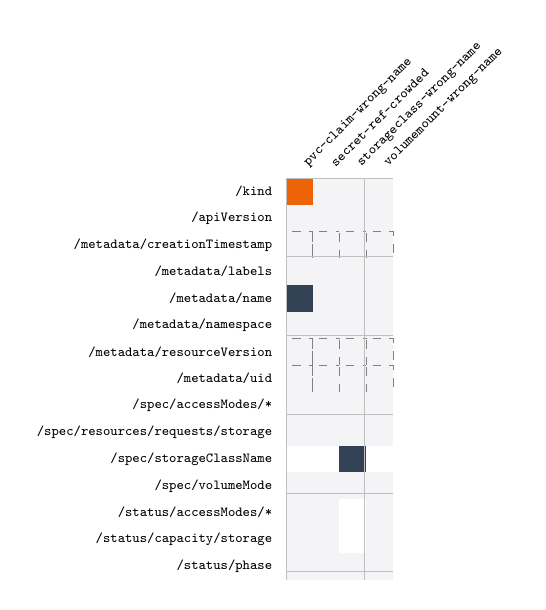
\begin{tikzpicture}[x=3.4mm,y=3.4mm]
\node[rotate=45,anchor=west,font=\ttfamily\tiny] at (0.5,0.25) {pvc-claim-wrong-name};
\node[rotate=45,anchor=west,font=\ttfamily\tiny] at (1.5,0.25) {secret-ref-crowded};
\node[rotate=45,anchor=west,font=\ttfamily\tiny] at (2.5,0.25) {storageclass-wrong-name};
\node[rotate=45,anchor=west,font=\ttfamily\tiny] at (3.5,0.25) {volumemount-wrong-name};
\node[anchor=east,font=\ttfamily\tiny] at (-0.15,-0.5) {/kind};
\fill[fill={rgb,255:red,237;green,99;blue,7}] (0,-1) rectangle ++(1,1);
\fill[fill={rgb,255:red,244;green,244;blue,246}] (1,-1) rectangle ++(1,1);
\fill[fill={rgb,255:red,244;green,244;blue,246}] (2,-1) rectangle ++(1,1);
\fill[fill={rgb,255:red,244;green,244;blue,246}] (3,-1) rectangle ++(1,1);
\node[anchor=east,font=\ttfamily\tiny] at (-0.15,-1.5) {/apiVersion};
\fill[fill={rgb,255:red,244;green,244;blue,246}] (0,-2) rectangle ++(1,1);
\fill[fill={rgb,255:red,244;green,244;blue,246}] (1,-2) rectangle ++(1,1);
\fill[fill={rgb,255:red,244;green,244;blue,246}] (2,-2) rectangle ++(1,1);
\fill[fill={rgb,255:red,244;green,244;blue,246}] (3,-2) rectangle ++(1,1);
\node[anchor=east,font=\ttfamily\tiny] at (-0.15,-2.5) {/metadata/creationTimestamp};
\fill[fill={rgb,255:red,244;green,244;blue,246}] (0,-3) rectangle ++(1,1);
\draw[gray,dashed,line width=0.2pt] (0,-3) rectangle ++(1,1);
\fill[fill={rgb,255:red,244;green,244;blue,246}] (1,-3) rectangle ++(1,1);
\draw[gray,dashed,line width=0.2pt] (1,-3) rectangle ++(1,1);
\fill[fill={rgb,255:red,244;green,244;blue,246}] (2,-3) rectangle ++(1,1);
\draw[gray,dashed,line width=0.2pt] (2,-3) rectangle ++(1,1);
\fill[fill={rgb,255:red,244;green,244;blue,246}] (3,-3) rectangle ++(1,1);
\draw[gray,dashed,line width=0.2pt] (3,-3) rectangle ++(1,1);
\node[anchor=east,font=\ttfamily\tiny] at (-0.15,-3.5) {/metadata/labels};
\fill[fill={rgb,255:red,244;green,244;blue,246}] (0,-4) rectangle ++(1,1);
\fill[fill={rgb,255:red,244;green,244;blue,246}] (1,-4) rectangle ++(1,1);
\fill[fill={rgb,255:red,244;green,244;blue,246}] (2,-4) rectangle ++(1,1);
\fill[fill={rgb,255:red,244;green,244;blue,246}] (3,-4) rectangle ++(1,1);
\node[anchor=east,font=\ttfamily\tiny] at (-0.15,-4.5) {/metadata/name};
\fill[fill={rgb,255:red,51;green,65;blue,85}] (0,-5) rectangle ++(1,1);
\node[white,font=\tiny] at (0.5,-5.5) {$\ast$};
\fill[fill={rgb,255:red,244;green,244;blue,246}] (1,-5) rectangle ++(1,1);
\fill[fill={rgb,255:red,244;green,244;blue,246}] (2,-5) rectangle ++(1,1);
\fill[fill={rgb,255:red,244;green,244;blue,246}] (3,-5) rectangle ++(1,1);
\node[anchor=east,font=\ttfamily\tiny] at (-0.15,-5.5) {/metadata/namespace};
\fill[fill={rgb,255:red,244;green,244;blue,246}] (0,-6) rectangle ++(1,1);
\fill[fill={rgb,255:red,244;green,244;blue,246}] (1,-6) rectangle ++(1,1);
\fill[fill={rgb,255:red,244;green,244;blue,246}] (2,-6) rectangle ++(1,1);
\fill[fill={rgb,255:red,244;green,244;blue,246}] (3,-6) rectangle ++(1,1);
\node[anchor=east,font=\ttfamily\tiny] at (-0.15,-6.5) {/metadata/resourceVersion};
\fill[fill={rgb,255:red,244;green,244;blue,246}] (0,-7) rectangle ++(1,1);
\draw[gray,dashed,line width=0.2pt] (0,-7) rectangle ++(1,1);
\fill[fill={rgb,255:red,244;green,244;blue,246}] (1,-7) rectangle ++(1,1);
\draw[gray,dashed,line width=0.2pt] (1,-7) rectangle ++(1,1);
\fill[fill={rgb,255:red,244;green,244;blue,246}] (2,-7) rectangle ++(1,1);
\draw[gray,dashed,line width=0.2pt] (2,-7) rectangle ++(1,1);
\fill[fill={rgb,255:red,244;green,244;blue,246}] (3,-7) rectangle ++(1,1);
\draw[gray,dashed,line width=0.2pt] (3,-7) rectangle ++(1,1);
\node[anchor=east,font=\ttfamily\tiny] at (-0.15,-7.5) {/metadata/uid};
\fill[fill={rgb,255:red,244;green,244;blue,246}] (0,-8) rectangle ++(1,1);
\draw[gray,dashed,line width=0.2pt] (0,-8) rectangle ++(1,1);
\fill[fill={rgb,255:red,244;green,244;blue,246}] (1,-8) rectangle ++(1,1);
\draw[gray,dashed,line width=0.2pt] (1,-8) rectangle ++(1,1);
\fill[fill={rgb,255:red,244;green,244;blue,246}] (2,-8) rectangle ++(1,1);
\draw[gray,dashed,line width=0.2pt] (2,-8) rectangle ++(1,1);
\fill[fill={rgb,255:red,244;green,244;blue,246}] (3,-8) rectangle ++(1,1);
\draw[gray,dashed,line width=0.2pt] (3,-8) rectangle ++(1,1);
\node[anchor=east,font=\ttfamily\tiny] at (-0.15,-8.5) {/spec/accessModes/*};
\fill[fill={rgb,255:red,244;green,244;blue,246}] (0,-9) rectangle ++(1,1);
\fill[fill={rgb,255:red,244;green,244;blue,246}] (1,-9) rectangle ++(1,1);
\fill[fill={rgb,255:red,244;green,244;blue,246}] (2,-9) rectangle ++(1,1);
\fill[fill={rgb,255:red,244;green,244;blue,246}] (3,-9) rectangle ++(1,1);
\node[anchor=east,font=\ttfamily\tiny] at (-0.15,-9.5) {/spec/resources/requests/storage};
\fill[fill={rgb,255:red,244;green,244;blue,246}] (0,-10) rectangle ++(1,1);
\fill[fill={rgb,255:red,244;green,244;blue,246}] (1,-10) rectangle ++(1,1);
\fill[fill={rgb,255:red,244;green,244;blue,246}] (2,-10) rectangle ++(1,1);
\fill[fill={rgb,255:red,244;green,244;blue,246}] (3,-10) rectangle ++(1,1);
\node[anchor=east,font=\ttfamily\tiny] at (-0.15,-10.5) {/spec/storageClassName};
\fill[fill={rgb,255:red,51;green,65;blue,85}] (2,-11) rectangle ++(1,1);
\node[white,font=\tiny] at (2.5,-11.5) {$\ast$};
\node[anchor=east,font=\ttfamily\tiny] at (-0.15,-11.5) {/spec/volumeMode};
\fill[fill={rgb,255:red,244;green,244;blue,246}] (0,-12) rectangle ++(1,1);
\fill[fill={rgb,255:red,244;green,244;blue,246}] (1,-12) rectangle ++(1,1);
\fill[fill={rgb,255:red,244;green,244;blue,246}] (2,-12) rectangle ++(1,1);
\fill[fill={rgb,255:red,244;green,244;blue,246}] (3,-12) rectangle ++(1,1);
\node[anchor=east,font=\ttfamily\tiny] at (-0.15,-12.5) {/status/accessModes/*};
\fill[fill={rgb,255:red,244;green,244;blue,246}] (0,-13) rectangle ++(1,1);
\fill[fill={rgb,255:red,244;green,244;blue,246}] (1,-13) rectangle ++(1,1);
\fill[fill={rgb,255:red,244;green,244;blue,246}] (3,-13) rectangle ++(1,1);
\node[anchor=east,font=\ttfamily\tiny] at (-0.15,-13.5) {/status/capacity/storage};
\fill[fill={rgb,255:red,244;green,244;blue,246}] (0,-14) rectangle ++(1,1);
\fill[fill={rgb,255:red,244;green,244;blue,246}] (1,-14) rectangle ++(1,1);
\fill[fill={rgb,255:red,244;green,244;blue,246}] (3,-14) rectangle ++(1,1);
\node[anchor=east,font=\ttfamily\tiny] at (-0.15,-14.5) {/status/phase};
\fill[fill={rgb,255:red,244;green,244;blue,246}] (0,-15) rectangle ++(1,1);
\fill[fill={rgb,255:red,244;green,244;blue,246}] (1,-15) rectangle ++(1,1);
\fill[fill={rgb,255:red,244;green,244;blue,246}] (2,-15) rectangle ++(1,1);
\fill[fill={rgb,255:red,244;green,244;blue,246}] (3,-15) rectangle ++(1,1);
\draw[gray!50,line width=0.2pt] (0,0) grid (4,-15);
\end{tikzpicture}

\par\medskip\noindent{\small\bfseries Role}\par\smallskip
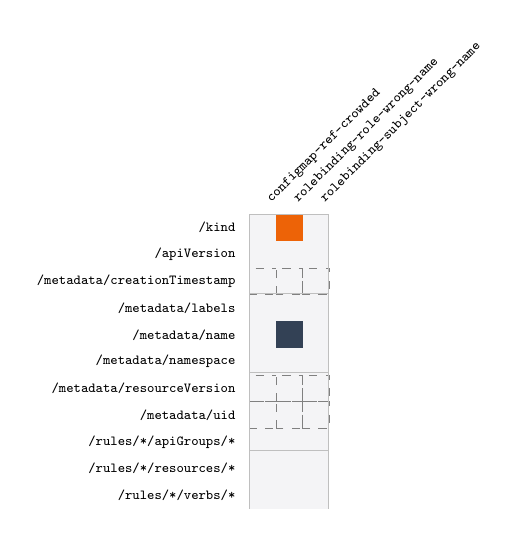
\begin{tikzpicture}[x=3.4mm,y=3.4mm]
\node[rotate=45,anchor=west,font=\ttfamily\tiny] at (0.5,0.25) {configmap-ref-crowded};
\node[rotate=45,anchor=west,font=\ttfamily\tiny] at (1.5,0.25) {rolebinding-role-wrong-name};
\node[rotate=45,anchor=west,font=\ttfamily\tiny] at (2.5,0.25) {rolebinding-subject-wrong-name};
\node[anchor=east,font=\ttfamily\tiny] at (-0.15,-0.5) {/kind};
\fill[fill={rgb,255:red,244;green,244;blue,246}] (0,-1) rectangle ++(1,1);
\fill[fill={rgb,255:red,237;green,99;blue,7}] (1,-1) rectangle ++(1,1);
\fill[fill={rgb,255:red,244;green,244;blue,246}] (2,-1) rectangle ++(1,1);
\node[anchor=east,font=\ttfamily\tiny] at (-0.15,-1.5) {/apiVersion};
\fill[fill={rgb,255:red,244;green,244;blue,246}] (0,-2) rectangle ++(1,1);
\fill[fill={rgb,255:red,244;green,244;blue,246}] (1,-2) rectangle ++(1,1);
\fill[fill={rgb,255:red,244;green,244;blue,246}] (2,-2) rectangle ++(1,1);
\node[anchor=east,font=\ttfamily\tiny] at (-0.15,-2.5) {/metadata/creationTimestamp};
\fill[fill={rgb,255:red,244;green,244;blue,246}] (0,-3) rectangle ++(1,1);
\draw[gray,dashed,line width=0.2pt] (0,-3) rectangle ++(1,1);
\fill[fill={rgb,255:red,244;green,244;blue,246}] (1,-3) rectangle ++(1,1);
\draw[gray,dashed,line width=0.2pt] (1,-3) rectangle ++(1,1);
\fill[fill={rgb,255:red,244;green,244;blue,246}] (2,-3) rectangle ++(1,1);
\draw[gray,dashed,line width=0.2pt] (2,-3) rectangle ++(1,1);
\node[anchor=east,font=\ttfamily\tiny] at (-0.15,-3.5) {/metadata/labels};
\fill[fill={rgb,255:red,244;green,244;blue,246}] (0,-4) rectangle ++(1,1);
\fill[fill={rgb,255:red,244;green,244;blue,246}] (1,-4) rectangle ++(1,1);
\fill[fill={rgb,255:red,244;green,244;blue,246}] (2,-4) rectangle ++(1,1);
\node[anchor=east,font=\ttfamily\tiny] at (-0.15,-4.5) {/metadata/name};
\fill[fill={rgb,255:red,244;green,244;blue,246}] (0,-5) rectangle ++(1,1);
\fill[fill={rgb,255:red,51;green,65;blue,85}] (1,-5) rectangle ++(1,1);
\node[white,font=\tiny] at (1.5,-5.5) {$\ast$};
\fill[fill={rgb,255:red,244;green,244;blue,246}] (2,-5) rectangle ++(1,1);
\node[anchor=east,font=\ttfamily\tiny] at (-0.15,-5.5) {/metadata/namespace};
\fill[fill={rgb,255:red,244;green,244;blue,246}] (0,-6) rectangle ++(1,1);
\fill[fill={rgb,255:red,244;green,244;blue,246}] (1,-6) rectangle ++(1,1);
\fill[fill={rgb,255:red,244;green,244;blue,246}] (2,-6) rectangle ++(1,1);
\node[anchor=east,font=\ttfamily\tiny] at (-0.15,-6.5) {/metadata/resourceVersion};
\fill[fill={rgb,255:red,244;green,244;blue,246}] (0,-7) rectangle ++(1,1);
\draw[gray,dashed,line width=0.2pt] (0,-7) rectangle ++(1,1);
\fill[fill={rgb,255:red,244;green,244;blue,246}] (1,-7) rectangle ++(1,1);
\draw[gray,dashed,line width=0.2pt] (1,-7) rectangle ++(1,1);
\fill[fill={rgb,255:red,244;green,244;blue,246}] (2,-7) rectangle ++(1,1);
\draw[gray,dashed,line width=0.2pt] (2,-7) rectangle ++(1,1);
\node[anchor=east,font=\ttfamily\tiny] at (-0.15,-7.5) {/metadata/uid};
\fill[fill={rgb,255:red,244;green,244;blue,246}] (0,-8) rectangle ++(1,1);
\draw[gray,dashed,line width=0.2pt] (0,-8) rectangle ++(1,1);
\fill[fill={rgb,255:red,244;green,244;blue,246}] (1,-8) rectangle ++(1,1);
\draw[gray,dashed,line width=0.2pt] (1,-8) rectangle ++(1,1);
\fill[fill={rgb,255:red,244;green,244;blue,246}] (2,-8) rectangle ++(1,1);
\draw[gray,dashed,line width=0.2pt] (2,-8) rectangle ++(1,1);
\node[anchor=east,font=\ttfamily\tiny] at (-0.15,-8.5) {/rules/*/apiGroups/*};
\fill[fill={rgb,255:red,244;green,244;blue,246}] (0,-9) rectangle ++(1,1);
\fill[fill={rgb,255:red,244;green,244;blue,246}] (1,-9) rectangle ++(1,1);
\fill[fill={rgb,255:red,244;green,244;blue,246}] (2,-9) rectangle ++(1,1);
\node[anchor=east,font=\ttfamily\tiny] at (-0.15,-9.5) {/rules/*/resources/*};
\fill[fill={rgb,255:red,244;green,244;blue,246}] (0,-10) rectangle ++(1,1);
\fill[fill={rgb,255:red,244;green,244;blue,246}] (1,-10) rectangle ++(1,1);
\fill[fill={rgb,255:red,244;green,244;blue,246}] (2,-10) rectangle ++(1,1);
\node[anchor=east,font=\ttfamily\tiny] at (-0.15,-10.5) {/rules/*/verbs/*};
\fill[fill={rgb,255:red,244;green,244;blue,246}] (0,-11) rectangle ++(1,1);
\fill[fill={rgb,255:red,244;green,244;blue,246}] (1,-11) rectangle ++(1,1);
\fill[fill={rgb,255:red,244;green,244;blue,246}] (2,-11) rectangle ++(1,1);
\draw[gray!50,line width=0.2pt] (0,0) grid (3,-11);
\end{tikzpicture}

\par\medskip\noindent{\small\bfseries Deployment}\par\smallskip
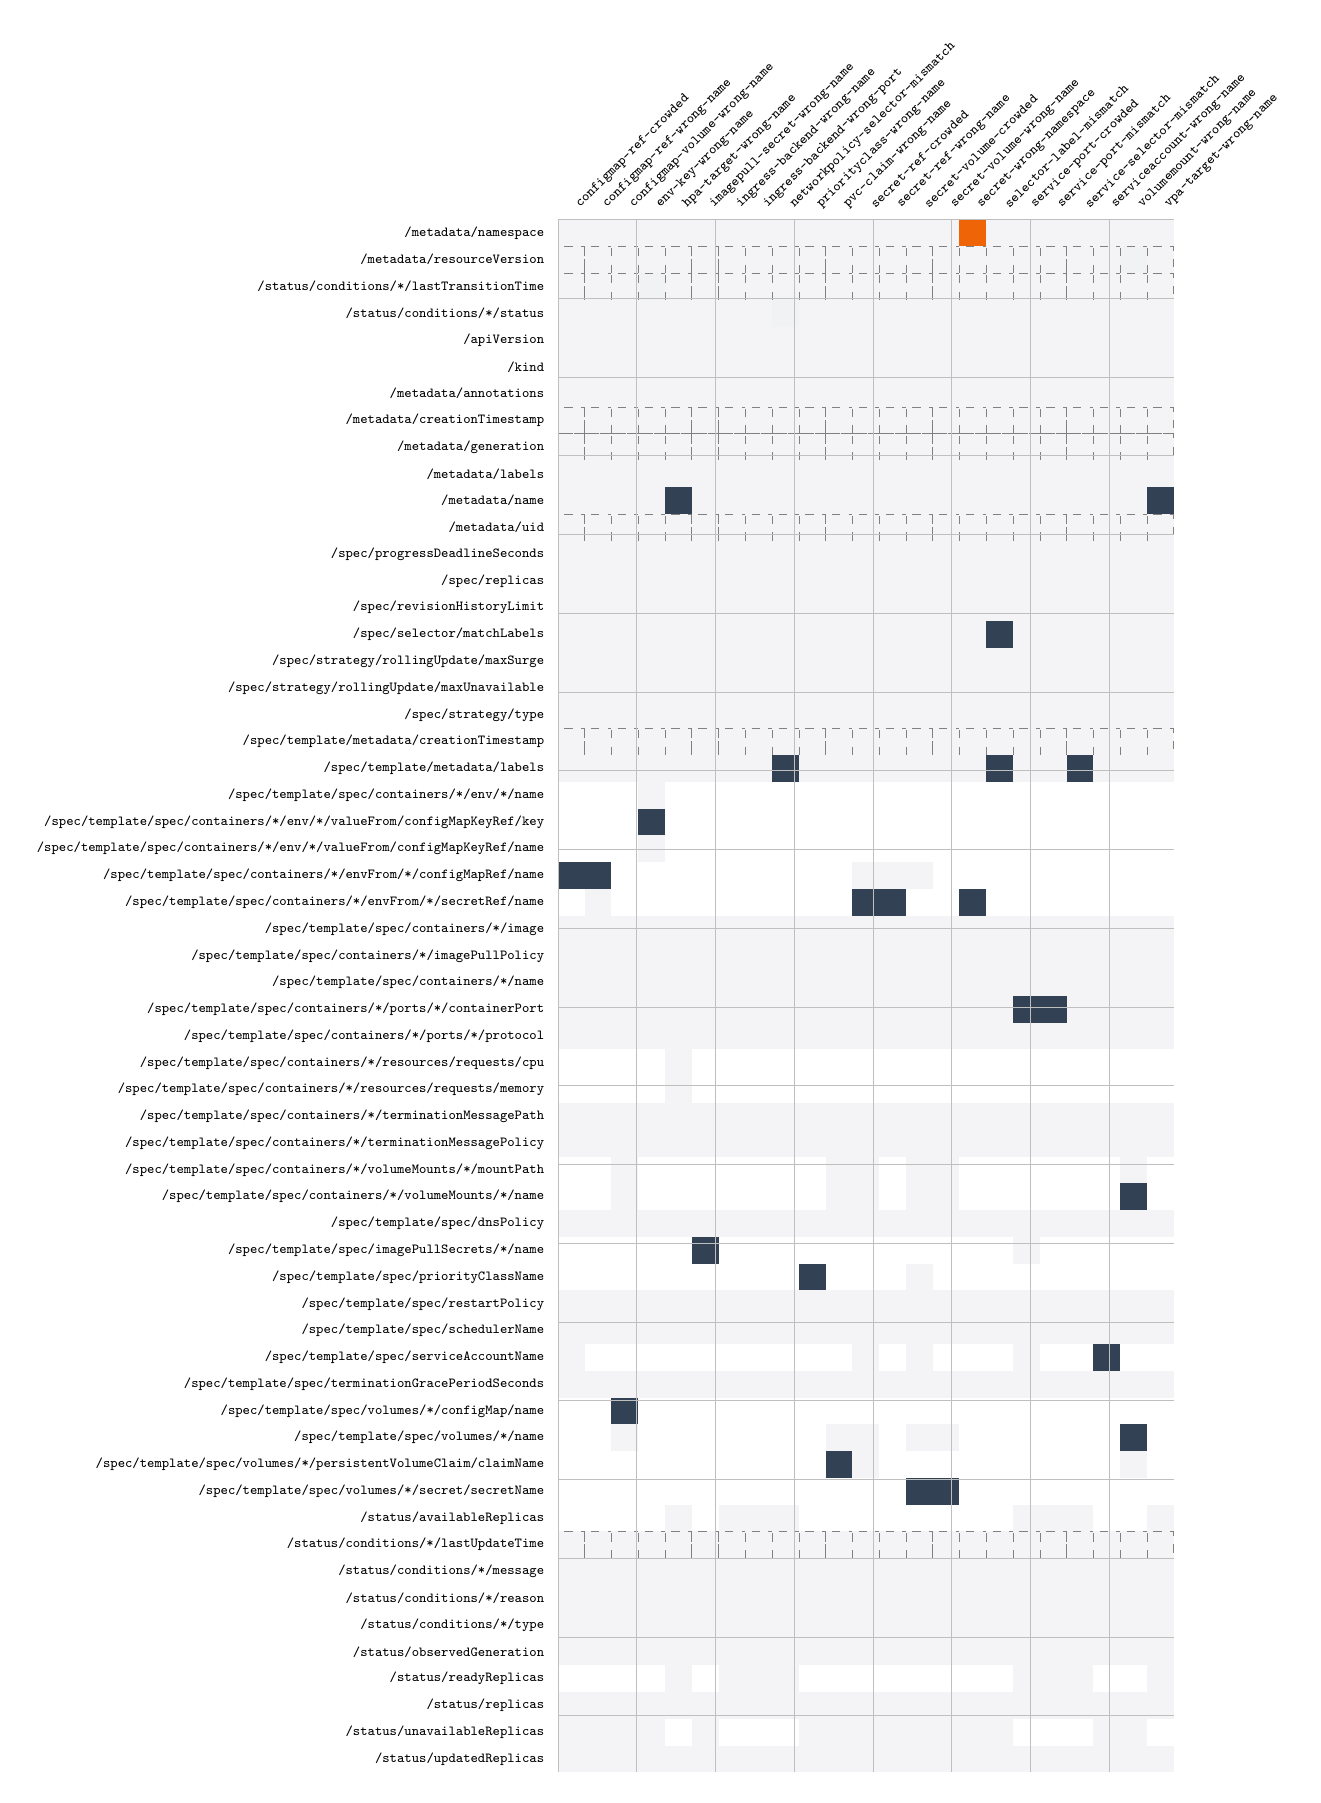
\begin{tikzpicture}[x=3.4mm,y=3.4mm]
\node[rotate=45,anchor=west,font=\ttfamily\tiny] at (0.5,0.25) {configmap-ref-crowded};
\node[rotate=45,anchor=west,font=\ttfamily\tiny] at (1.5,0.25) {configmap-ref-wrong-name};
\node[rotate=45,anchor=west,font=\ttfamily\tiny] at (2.5,0.25) {configmap-volume-wrong-name};
\node[rotate=45,anchor=west,font=\ttfamily\tiny] at (3.5,0.25) {env-key-wrong-name};
\node[rotate=45,anchor=west,font=\ttfamily\tiny] at (4.5,0.25) {hpa-target-wrong-name};
\node[rotate=45,anchor=west,font=\ttfamily\tiny] at (5.5,0.25) {imagepull-secret-wrong-name};
\node[rotate=45,anchor=west,font=\ttfamily\tiny] at (6.5,0.25) {ingress-backend-wrong-name};
\node[rotate=45,anchor=west,font=\ttfamily\tiny] at (7.5,0.25) {ingress-backend-wrong-port};
\node[rotate=45,anchor=west,font=\ttfamily\tiny] at (8.5,0.25) {networkpolicy-selector-mismatch};
\node[rotate=45,anchor=west,font=\ttfamily\tiny] at (9.5,0.25) {priorityclass-wrong-name};
\node[rotate=45,anchor=west,font=\ttfamily\tiny] at (10.5,0.25) {pvc-claim-wrong-name};
\node[rotate=45,anchor=west,font=\ttfamily\tiny] at (11.5,0.25) {secret-ref-crowded};
\node[rotate=45,anchor=west,font=\ttfamily\tiny] at (12.5,0.25) {secret-ref-wrong-name};
\node[rotate=45,anchor=west,font=\ttfamily\tiny] at (13.5,0.25) {secret-volume-crowded};
\node[rotate=45,anchor=west,font=\ttfamily\tiny] at (14.5,0.25) {secret-volume-wrong-name};
\node[rotate=45,anchor=west,font=\ttfamily\tiny] at (15.5,0.25) {secret-wrong-namespace};
\node[rotate=45,anchor=west,font=\ttfamily\tiny] at (16.5,0.25) {selector-label-mismatch};
\node[rotate=45,anchor=west,font=\ttfamily\tiny] at (17.5,0.25) {service-port-crowded};
\node[rotate=45,anchor=west,font=\ttfamily\tiny] at (18.5,0.25) {service-port-mismatch};
\node[rotate=45,anchor=west,font=\ttfamily\tiny] at (19.5,0.25) {service-selector-mismatch};
\node[rotate=45,anchor=west,font=\ttfamily\tiny] at (20.5,0.25) {serviceaccount-wrong-name};
\node[rotate=45,anchor=west,font=\ttfamily\tiny] at (21.5,0.25) {volumemount-wrong-name};
\node[rotate=45,anchor=west,font=\ttfamily\tiny] at (22.5,0.25) {vpa-target-wrong-name};
\node[anchor=east,font=\ttfamily\tiny] at (-0.15,-0.5) {/metadata/namespace};
\fill[fill={rgb,255:red,244;green,244;blue,246}] (0,-1) rectangle ++(1,1);
\fill[fill={rgb,255:red,244;green,244;blue,246}] (1,-1) rectangle ++(1,1);
\fill[fill={rgb,255:red,244;green,244;blue,246}] (2,-1) rectangle ++(1,1);
\fill[fill={rgb,255:red,244;green,244;blue,246}] (3,-1) rectangle ++(1,1);
\fill[fill={rgb,255:red,244;green,244;blue,246}] (4,-1) rectangle ++(1,1);
\fill[fill={rgb,255:red,244;green,244;blue,246}] (5,-1) rectangle ++(1,1);
\fill[fill={rgb,255:red,244;green,244;blue,246}] (6,-1) rectangle ++(1,1);
\fill[fill={rgb,255:red,244;green,244;blue,246}] (7,-1) rectangle ++(1,1);
\fill[fill={rgb,255:red,244;green,244;blue,246}] (8,-1) rectangle ++(1,1);
\fill[fill={rgb,255:red,244;green,244;blue,246}] (9,-1) rectangle ++(1,1);
\fill[fill={rgb,255:red,244;green,244;blue,246}] (10,-1) rectangle ++(1,1);
\fill[fill={rgb,255:red,244;green,244;blue,246}] (11,-1) rectangle ++(1,1);
\fill[fill={rgb,255:red,244;green,244;blue,246}] (12,-1) rectangle ++(1,1);
\fill[fill={rgb,255:red,244;green,244;blue,246}] (13,-1) rectangle ++(1,1);
\fill[fill={rgb,255:red,244;green,244;blue,246}] (14,-1) rectangle ++(1,1);
\fill[fill={rgb,255:red,239;green,100;blue,7}] (15,-1) rectangle ++(1,1);
\fill[fill={rgb,255:red,244;green,244;blue,246}] (16,-1) rectangle ++(1,1);
\fill[fill={rgb,255:red,244;green,244;blue,246}] (17,-1) rectangle ++(1,1);
\fill[fill={rgb,255:red,244;green,244;blue,246}] (18,-1) rectangle ++(1,1);
\fill[fill={rgb,255:red,244;green,244;blue,246}] (19,-1) rectangle ++(1,1);
\fill[fill={rgb,255:red,244;green,244;blue,246}] (20,-1) rectangle ++(1,1);
\fill[fill={rgb,255:red,244;green,244;blue,246}] (21,-1) rectangle ++(1,1);
\fill[fill={rgb,255:red,244;green,244;blue,246}] (22,-1) rectangle ++(1,1);
\node[anchor=east,font=\ttfamily\tiny] at (-0.15,-1.5) {/metadata/resourceVersion};
\fill[fill={rgb,255:red,244;green,244;blue,246}] (0,-2) rectangle ++(1,1);
\draw[gray,dashed,line width=0.2pt] (0,-2) rectangle ++(1,1);
\fill[fill={rgb,255:red,244;green,244;blue,246}] (1,-2) rectangle ++(1,1);
\draw[gray,dashed,line width=0.2pt] (1,-2) rectangle ++(1,1);
\fill[fill={rgb,255:red,244;green,244;blue,246}] (2,-2) rectangle ++(1,1);
\draw[gray,dashed,line width=0.2pt] (2,-2) rectangle ++(1,1);
\fill[fill={rgb,255:red,244;green,244;blue,246}] (3,-2) rectangle ++(1,1);
\draw[gray,dashed,line width=0.2pt] (3,-2) rectangle ++(1,1);
\fill[fill={rgb,255:red,244;green,244;blue,246}] (4,-2) rectangle ++(1,1);
\draw[gray,dashed,line width=0.2pt] (4,-2) rectangle ++(1,1);
\fill[fill={rgb,255:red,244;green,244;blue,246}] (5,-2) rectangle ++(1,1);
\draw[gray,dashed,line width=0.2pt] (5,-2) rectangle ++(1,1);
\fill[fill={rgb,255:red,244;green,244;blue,246}] (6,-2) rectangle ++(1,1);
\draw[gray,dashed,line width=0.2pt] (6,-2) rectangle ++(1,1);
\fill[fill={rgb,255:red,244;green,244;blue,246}] (7,-2) rectangle ++(1,1);
\draw[gray,dashed,line width=0.2pt] (7,-2) rectangle ++(1,1);
\fill[fill={rgb,255:red,244;green,244;blue,246}] (8,-2) rectangle ++(1,1);
\draw[gray,dashed,line width=0.2pt] (8,-2) rectangle ++(1,1);
\fill[fill={rgb,255:red,244;green,244;blue,246}] (9,-2) rectangle ++(1,1);
\draw[gray,dashed,line width=0.2pt] (9,-2) rectangle ++(1,1);
\fill[fill={rgb,255:red,244;green,244;blue,246}] (10,-2) rectangle ++(1,1);
\draw[gray,dashed,line width=0.2pt] (10,-2) rectangle ++(1,1);
\fill[fill={rgb,255:red,244;green,244;blue,246}] (11,-2) rectangle ++(1,1);
\draw[gray,dashed,line width=0.2pt] (11,-2) rectangle ++(1,1);
\fill[fill={rgb,255:red,244;green,244;blue,246}] (12,-2) rectangle ++(1,1);
\draw[gray,dashed,line width=0.2pt] (12,-2) rectangle ++(1,1);
\fill[fill={rgb,255:red,244;green,244;blue,246}] (13,-2) rectangle ++(1,1);
\draw[gray,dashed,line width=0.2pt] (13,-2) rectangle ++(1,1);
\fill[fill={rgb,255:red,244;green,244;blue,246}] (14,-2) rectangle ++(1,1);
\draw[gray,dashed,line width=0.2pt] (14,-2) rectangle ++(1,1);
\fill[fill={rgb,255:red,244;green,244;blue,246}] (15,-2) rectangle ++(1,1);
\draw[gray,dashed,line width=0.2pt] (15,-2) rectangle ++(1,1);
\fill[fill={rgb,255:red,244;green,244;blue,246}] (16,-2) rectangle ++(1,1);
\draw[gray,dashed,line width=0.2pt] (16,-2) rectangle ++(1,1);
\fill[fill={rgb,255:red,244;green,244;blue,246}] (17,-2) rectangle ++(1,1);
\draw[gray,dashed,line width=0.2pt] (17,-2) rectangle ++(1,1);
\fill[fill={rgb,255:red,244;green,244;blue,246}] (18,-2) rectangle ++(1,1);
\draw[gray,dashed,line width=0.2pt] (18,-2) rectangle ++(1,1);
\fill[fill={rgb,255:red,244;green,244;blue,246}] (19,-2) rectangle ++(1,1);
\draw[gray,dashed,line width=0.2pt] (19,-2) rectangle ++(1,1);
\fill[fill={rgb,255:red,244;green,244;blue,246}] (20,-2) rectangle ++(1,1);
\draw[gray,dashed,line width=0.2pt] (20,-2) rectangle ++(1,1);
\fill[fill={rgb,255:red,241;green,242;blue,243}] (21,-2) rectangle ++(1,1);
\draw[gray,dashed,line width=0.2pt] (21,-2) rectangle ++(1,1);
\fill[fill={rgb,255:red,244;green,244;blue,246}] (22,-2) rectangle ++(1,1);
\draw[gray,dashed,line width=0.2pt] (22,-2) rectangle ++(1,1);
\node[anchor=east,font=\ttfamily\tiny] at (-0.15,-2.5) {/status/conditions/*/lastTransitionTime};
\fill[fill={rgb,255:red,244;green,244;blue,246}] (0,-3) rectangle ++(1,1);
\draw[gray,dashed,line width=0.2pt] (0,-3) rectangle ++(1,1);
\fill[fill={rgb,255:red,244;green,244;blue,246}] (1,-3) rectangle ++(1,1);
\draw[gray,dashed,line width=0.2pt] (1,-3) rectangle ++(1,1);
\fill[fill={rgb,255:red,244;green,244;blue,246}] (2,-3) rectangle ++(1,1);
\draw[gray,dashed,line width=0.2pt] (2,-3) rectangle ++(1,1);
\fill[fill={rgb,255:red,241;green,242;blue,243}] (3,-3) rectangle ++(1,1);
\draw[gray,dashed,line width=0.2pt] (3,-3) rectangle ++(1,1);
\fill[fill={rgb,255:red,244;green,244;blue,246}] (4,-3) rectangle ++(1,1);
\draw[gray,dashed,line width=0.2pt] (4,-3) rectangle ++(1,1);
\fill[fill={rgb,255:red,244;green,244;blue,246}] (5,-3) rectangle ++(1,1);
\draw[gray,dashed,line width=0.2pt] (5,-3) rectangle ++(1,1);
\fill[fill={rgb,255:red,244;green,244;blue,246}] (6,-3) rectangle ++(1,1);
\draw[gray,dashed,line width=0.2pt] (6,-3) rectangle ++(1,1);
\fill[fill={rgb,255:red,244;green,244;blue,246}] (7,-3) rectangle ++(1,1);
\draw[gray,dashed,line width=0.2pt] (7,-3) rectangle ++(1,1);
\fill[fill={rgb,255:red,244;green,244;blue,246}] (8,-3) rectangle ++(1,1);
\draw[gray,dashed,line width=0.2pt] (8,-3) rectangle ++(1,1);
\fill[fill={rgb,255:red,244;green,244;blue,246}] (9,-3) rectangle ++(1,1);
\draw[gray,dashed,line width=0.2pt] (9,-3) rectangle ++(1,1);
\fill[fill={rgb,255:red,244;green,244;blue,246}] (10,-3) rectangle ++(1,1);
\draw[gray,dashed,line width=0.2pt] (10,-3) rectangle ++(1,1);
\fill[fill={rgb,255:red,244;green,244;blue,246}] (11,-3) rectangle ++(1,1);
\draw[gray,dashed,line width=0.2pt] (11,-3) rectangle ++(1,1);
\fill[fill={rgb,255:red,244;green,244;blue,246}] (12,-3) rectangle ++(1,1);
\draw[gray,dashed,line width=0.2pt] (12,-3) rectangle ++(1,1);
\fill[fill={rgb,255:red,244;green,244;blue,246}] (13,-3) rectangle ++(1,1);
\draw[gray,dashed,line width=0.2pt] (13,-3) rectangle ++(1,1);
\fill[fill={rgb,255:red,244;green,244;blue,246}] (14,-3) rectangle ++(1,1);
\draw[gray,dashed,line width=0.2pt] (14,-3) rectangle ++(1,1);
\fill[fill={rgb,255:red,244;green,244;blue,246}] (15,-3) rectangle ++(1,1);
\draw[gray,dashed,line width=0.2pt] (15,-3) rectangle ++(1,1);
\fill[fill={rgb,255:red,244;green,244;blue,246}] (16,-3) rectangle ++(1,1);
\draw[gray,dashed,line width=0.2pt] (16,-3) rectangle ++(1,1);
\fill[fill={rgb,255:red,244;green,244;blue,246}] (17,-3) rectangle ++(1,1);
\draw[gray,dashed,line width=0.2pt] (17,-3) rectangle ++(1,1);
\fill[fill={rgb,255:red,244;green,244;blue,246}] (18,-3) rectangle ++(1,1);
\draw[gray,dashed,line width=0.2pt] (18,-3) rectangle ++(1,1);
\fill[fill={rgb,255:red,244;green,244;blue,246}] (19,-3) rectangle ++(1,1);
\draw[gray,dashed,line width=0.2pt] (19,-3) rectangle ++(1,1);
\fill[fill={rgb,255:red,244;green,244;blue,246}] (20,-3) rectangle ++(1,1);
\draw[gray,dashed,line width=0.2pt] (20,-3) rectangle ++(1,1);
\fill[fill={rgb,255:red,244;green,244;blue,246}] (21,-3) rectangle ++(1,1);
\draw[gray,dashed,line width=0.2pt] (21,-3) rectangle ++(1,1);
\fill[fill={rgb,255:red,244;green,244;blue,246}] (22,-3) rectangle ++(1,1);
\draw[gray,dashed,line width=0.2pt] (22,-3) rectangle ++(1,1);
\node[anchor=east,font=\ttfamily\tiny] at (-0.15,-3.5) {/status/conditions/*/status};
\fill[fill={rgb,255:red,244;green,244;blue,246}] (0,-4) rectangle ++(1,1);
\fill[fill={rgb,255:red,244;green,244;blue,246}] (1,-4) rectangle ++(1,1);
\fill[fill={rgb,255:red,244;green,244;blue,246}] (2,-4) rectangle ++(1,1);
\fill[fill={rgb,255:red,244;green,244;blue,246}] (3,-4) rectangle ++(1,1);
\fill[fill={rgb,255:red,244;green,244;blue,246}] (4,-4) rectangle ++(1,1);
\fill[fill={rgb,255:red,244;green,244;blue,246}] (5,-4) rectangle ++(1,1);
\fill[fill={rgb,255:red,244;green,244;blue,246}] (6,-4) rectangle ++(1,1);
\fill[fill={rgb,255:red,244;green,244;blue,246}] (7,-4) rectangle ++(1,1);
\fill[fill={rgb,255:red,241;green,242;blue,243}] (8,-4) rectangle ++(1,1);
\fill[fill={rgb,255:red,244;green,244;blue,246}] (9,-4) rectangle ++(1,1);
\fill[fill={rgb,255:red,244;green,244;blue,246}] (10,-4) rectangle ++(1,1);
\fill[fill={rgb,255:red,244;green,244;blue,246}] (11,-4) rectangle ++(1,1);
\fill[fill={rgb,255:red,244;green,244;blue,246}] (12,-4) rectangle ++(1,1);
\fill[fill={rgb,255:red,244;green,244;blue,246}] (13,-4) rectangle ++(1,1);
\fill[fill={rgb,255:red,244;green,244;blue,246}] (14,-4) rectangle ++(1,1);
\fill[fill={rgb,255:red,244;green,244;blue,246}] (15,-4) rectangle ++(1,1);
\fill[fill={rgb,255:red,244;green,244;blue,246}] (16,-4) rectangle ++(1,1);
\fill[fill={rgb,255:red,244;green,244;blue,246}] (17,-4) rectangle ++(1,1);
\fill[fill={rgb,255:red,244;green,244;blue,246}] (18,-4) rectangle ++(1,1);
\fill[fill={rgb,255:red,244;green,244;blue,246}] (19,-4) rectangle ++(1,1);
\fill[fill={rgb,255:red,244;green,244;blue,246}] (20,-4) rectangle ++(1,1);
\fill[fill={rgb,255:red,244;green,244;blue,246}] (21,-4) rectangle ++(1,1);
\fill[fill={rgb,255:red,244;green,244;blue,246}] (22,-4) rectangle ++(1,1);
\node[anchor=east,font=\ttfamily\tiny] at (-0.15,-4.5) {/apiVersion};
\fill[fill={rgb,255:red,244;green,244;blue,246}] (0,-5) rectangle ++(1,1);
\fill[fill={rgb,255:red,244;green,244;blue,246}] (1,-5) rectangle ++(1,1);
\fill[fill={rgb,255:red,244;green,244;blue,246}] (2,-5) rectangle ++(1,1);
\fill[fill={rgb,255:red,244;green,244;blue,246}] (3,-5) rectangle ++(1,1);
\fill[fill={rgb,255:red,244;green,244;blue,246}] (4,-5) rectangle ++(1,1);
\fill[fill={rgb,255:red,244;green,244;blue,246}] (5,-5) rectangle ++(1,1);
\fill[fill={rgb,255:red,244;green,244;blue,246}] (6,-5) rectangle ++(1,1);
\fill[fill={rgb,255:red,244;green,244;blue,246}] (7,-5) rectangle ++(1,1);
\fill[fill={rgb,255:red,244;green,244;blue,246}] (8,-5) rectangle ++(1,1);
\fill[fill={rgb,255:red,244;green,244;blue,246}] (9,-5) rectangle ++(1,1);
\fill[fill={rgb,255:red,244;green,244;blue,246}] (10,-5) rectangle ++(1,1);
\fill[fill={rgb,255:red,244;green,244;blue,246}] (11,-5) rectangle ++(1,1);
\fill[fill={rgb,255:red,244;green,244;blue,246}] (12,-5) rectangle ++(1,1);
\fill[fill={rgb,255:red,244;green,244;blue,246}] (13,-5) rectangle ++(1,1);
\fill[fill={rgb,255:red,244;green,244;blue,246}] (14,-5) rectangle ++(1,1);
\fill[fill={rgb,255:red,244;green,244;blue,246}] (15,-5) rectangle ++(1,1);
\fill[fill={rgb,255:red,244;green,244;blue,246}] (16,-5) rectangle ++(1,1);
\fill[fill={rgb,255:red,244;green,244;blue,246}] (17,-5) rectangle ++(1,1);
\fill[fill={rgb,255:red,244;green,244;blue,246}] (18,-5) rectangle ++(1,1);
\fill[fill={rgb,255:red,244;green,244;blue,246}] (19,-5) rectangle ++(1,1);
\fill[fill={rgb,255:red,244;green,244;blue,246}] (20,-5) rectangle ++(1,1);
\fill[fill={rgb,255:red,244;green,244;blue,246}] (21,-5) rectangle ++(1,1);
\fill[fill={rgb,255:red,244;green,244;blue,246}] (22,-5) rectangle ++(1,1);
\node[anchor=east,font=\ttfamily\tiny] at (-0.15,-5.5) {/kind};
\fill[fill={rgb,255:red,244;green,244;blue,246}] (0,-6) rectangle ++(1,1);
\fill[fill={rgb,255:red,244;green,244;blue,246}] (1,-6) rectangle ++(1,1);
\fill[fill={rgb,255:red,244;green,244;blue,246}] (2,-6) rectangle ++(1,1);
\fill[fill={rgb,255:red,244;green,244;blue,246}] (3,-6) rectangle ++(1,1);
\fill[fill={rgb,255:red,244;green,244;blue,246}] (4,-6) rectangle ++(1,1);
\fill[fill={rgb,255:red,244;green,244;blue,246}] (5,-6) rectangle ++(1,1);
\fill[fill={rgb,255:red,244;green,244;blue,246}] (6,-6) rectangle ++(1,1);
\fill[fill={rgb,255:red,244;green,244;blue,246}] (7,-6) rectangle ++(1,1);
\fill[fill={rgb,255:red,244;green,244;blue,246}] (8,-6) rectangle ++(1,1);
\fill[fill={rgb,255:red,244;green,244;blue,246}] (9,-6) rectangle ++(1,1);
\fill[fill={rgb,255:red,244;green,244;blue,246}] (10,-6) rectangle ++(1,1);
\fill[fill={rgb,255:red,244;green,244;blue,246}] (11,-6) rectangle ++(1,1);
\fill[fill={rgb,255:red,244;green,244;blue,246}] (12,-6) rectangle ++(1,1);
\fill[fill={rgb,255:red,244;green,244;blue,246}] (13,-6) rectangle ++(1,1);
\fill[fill={rgb,255:red,244;green,244;blue,246}] (14,-6) rectangle ++(1,1);
\fill[fill={rgb,255:red,244;green,244;blue,246}] (15,-6) rectangle ++(1,1);
\fill[fill={rgb,255:red,244;green,244;blue,246}] (16,-6) rectangle ++(1,1);
\fill[fill={rgb,255:red,244;green,244;blue,246}] (17,-6) rectangle ++(1,1);
\fill[fill={rgb,255:red,244;green,244;blue,246}] (18,-6) rectangle ++(1,1);
\fill[fill={rgb,255:red,244;green,244;blue,246}] (19,-6) rectangle ++(1,1);
\fill[fill={rgb,255:red,244;green,244;blue,246}] (20,-6) rectangle ++(1,1);
\fill[fill={rgb,255:red,244;green,244;blue,246}] (21,-6) rectangle ++(1,1);
\fill[fill={rgb,255:red,244;green,244;blue,246}] (22,-6) rectangle ++(1,1);
\node[anchor=east,font=\ttfamily\tiny] at (-0.15,-6.5) {/metadata/annotations};
\fill[fill={rgb,255:red,244;green,244;blue,246}] (0,-7) rectangle ++(1,1);
\fill[fill={rgb,255:red,244;green,244;blue,246}] (1,-7) rectangle ++(1,1);
\fill[fill={rgb,255:red,244;green,244;blue,246}] (2,-7) rectangle ++(1,1);
\fill[fill={rgb,255:red,244;green,244;blue,246}] (3,-7) rectangle ++(1,1);
\fill[fill={rgb,255:red,244;green,244;blue,246}] (4,-7) rectangle ++(1,1);
\fill[fill={rgb,255:red,244;green,244;blue,246}] (5,-7) rectangle ++(1,1);
\fill[fill={rgb,255:red,244;green,244;blue,246}] (6,-7) rectangle ++(1,1);
\fill[fill={rgb,255:red,244;green,244;blue,246}] (7,-7) rectangle ++(1,1);
\fill[fill={rgb,255:red,244;green,244;blue,246}] (8,-7) rectangle ++(1,1);
\fill[fill={rgb,255:red,244;green,244;blue,246}] (9,-7) rectangle ++(1,1);
\fill[fill={rgb,255:red,244;green,244;blue,246}] (10,-7) rectangle ++(1,1);
\fill[fill={rgb,255:red,244;green,244;blue,246}] (11,-7) rectangle ++(1,1);
\fill[fill={rgb,255:red,244;green,244;blue,246}] (12,-7) rectangle ++(1,1);
\fill[fill={rgb,255:red,244;green,244;blue,246}] (13,-7) rectangle ++(1,1);
\fill[fill={rgb,255:red,244;green,244;blue,246}] (14,-7) rectangle ++(1,1);
\fill[fill={rgb,255:red,244;green,244;blue,246}] (15,-7) rectangle ++(1,1);
\fill[fill={rgb,255:red,244;green,244;blue,246}] (16,-7) rectangle ++(1,1);
\fill[fill={rgb,255:red,244;green,244;blue,246}] (17,-7) rectangle ++(1,1);
\fill[fill={rgb,255:red,244;green,244;blue,246}] (18,-7) rectangle ++(1,1);
\fill[fill={rgb,255:red,244;green,244;blue,246}] (19,-7) rectangle ++(1,1);
\fill[fill={rgb,255:red,244;green,244;blue,246}] (20,-7) rectangle ++(1,1);
\fill[fill={rgb,255:red,244;green,244;blue,246}] (21,-7) rectangle ++(1,1);
\fill[fill={rgb,255:red,244;green,244;blue,246}] (22,-7) rectangle ++(1,1);
\node[anchor=east,font=\ttfamily\tiny] at (-0.15,-7.5) {/metadata/creationTimestamp};
\fill[fill={rgb,255:red,244;green,244;blue,246}] (0,-8) rectangle ++(1,1);
\draw[gray,dashed,line width=0.2pt] (0,-8) rectangle ++(1,1);
\fill[fill={rgb,255:red,244;green,244;blue,246}] (1,-8) rectangle ++(1,1);
\draw[gray,dashed,line width=0.2pt] (1,-8) rectangle ++(1,1);
\fill[fill={rgb,255:red,244;green,244;blue,246}] (2,-8) rectangle ++(1,1);
\draw[gray,dashed,line width=0.2pt] (2,-8) rectangle ++(1,1);
\fill[fill={rgb,255:red,244;green,244;blue,246}] (3,-8) rectangle ++(1,1);
\draw[gray,dashed,line width=0.2pt] (3,-8) rectangle ++(1,1);
\fill[fill={rgb,255:red,244;green,244;blue,246}] (4,-8) rectangle ++(1,1);
\draw[gray,dashed,line width=0.2pt] (4,-8) rectangle ++(1,1);
\fill[fill={rgb,255:red,244;green,244;blue,246}] (5,-8) rectangle ++(1,1);
\draw[gray,dashed,line width=0.2pt] (5,-8) rectangle ++(1,1);
\fill[fill={rgb,255:red,244;green,244;blue,246}] (6,-8) rectangle ++(1,1);
\draw[gray,dashed,line width=0.2pt] (6,-8) rectangle ++(1,1);
\fill[fill={rgb,255:red,244;green,244;blue,246}] (7,-8) rectangle ++(1,1);
\draw[gray,dashed,line width=0.2pt] (7,-8) rectangle ++(1,1);
\fill[fill={rgb,255:red,244;green,244;blue,246}] (8,-8) rectangle ++(1,1);
\draw[gray,dashed,line width=0.2pt] (8,-8) rectangle ++(1,1);
\fill[fill={rgb,255:red,244;green,244;blue,246}] (9,-8) rectangle ++(1,1);
\draw[gray,dashed,line width=0.2pt] (9,-8) rectangle ++(1,1);
\fill[fill={rgb,255:red,244;green,244;blue,246}] (10,-8) rectangle ++(1,1);
\draw[gray,dashed,line width=0.2pt] (10,-8) rectangle ++(1,1);
\fill[fill={rgb,255:red,244;green,244;blue,246}] (11,-8) rectangle ++(1,1);
\draw[gray,dashed,line width=0.2pt] (11,-8) rectangle ++(1,1);
\fill[fill={rgb,255:red,244;green,244;blue,246}] (12,-8) rectangle ++(1,1);
\draw[gray,dashed,line width=0.2pt] (12,-8) rectangle ++(1,1);
\fill[fill={rgb,255:red,244;green,244;blue,246}] (13,-8) rectangle ++(1,1);
\draw[gray,dashed,line width=0.2pt] (13,-8) rectangle ++(1,1);
\fill[fill={rgb,255:red,244;green,244;blue,246}] (14,-8) rectangle ++(1,1);
\draw[gray,dashed,line width=0.2pt] (14,-8) rectangle ++(1,1);
\fill[fill={rgb,255:red,244;green,244;blue,246}] (15,-8) rectangle ++(1,1);
\draw[gray,dashed,line width=0.2pt] (15,-8) rectangle ++(1,1);
\fill[fill={rgb,255:red,244;green,244;blue,246}] (16,-8) rectangle ++(1,1);
\draw[gray,dashed,line width=0.2pt] (16,-8) rectangle ++(1,1);
\fill[fill={rgb,255:red,244;green,244;blue,246}] (17,-8) rectangle ++(1,1);
\draw[gray,dashed,line width=0.2pt] (17,-8) rectangle ++(1,1);
\fill[fill={rgb,255:red,244;green,244;blue,246}] (18,-8) rectangle ++(1,1);
\draw[gray,dashed,line width=0.2pt] (18,-8) rectangle ++(1,1);
\fill[fill={rgb,255:red,244;green,244;blue,246}] (19,-8) rectangle ++(1,1);
\draw[gray,dashed,line width=0.2pt] (19,-8) rectangle ++(1,1);
\fill[fill={rgb,255:red,244;green,244;blue,246}] (20,-8) rectangle ++(1,1);
\draw[gray,dashed,line width=0.2pt] (20,-8) rectangle ++(1,1);
\fill[fill={rgb,255:red,244;green,244;blue,246}] (21,-8) rectangle ++(1,1);
\draw[gray,dashed,line width=0.2pt] (21,-8) rectangle ++(1,1);
\fill[fill={rgb,255:red,244;green,244;blue,246}] (22,-8) rectangle ++(1,1);
\draw[gray,dashed,line width=0.2pt] (22,-8) rectangle ++(1,1);
\node[anchor=east,font=\ttfamily\tiny] at (-0.15,-8.5) {/metadata/generation};
\fill[fill={rgb,255:red,244;green,244;blue,246}] (0,-9) rectangle ++(1,1);
\draw[gray,dashed,line width=0.2pt] (0,-9) rectangle ++(1,1);
\fill[fill={rgb,255:red,244;green,244;blue,246}] (1,-9) rectangle ++(1,1);
\draw[gray,dashed,line width=0.2pt] (1,-9) rectangle ++(1,1);
\fill[fill={rgb,255:red,244;green,244;blue,246}] (2,-9) rectangle ++(1,1);
\draw[gray,dashed,line width=0.2pt] (2,-9) rectangle ++(1,1);
\fill[fill={rgb,255:red,244;green,244;blue,246}] (3,-9) rectangle ++(1,1);
\draw[gray,dashed,line width=0.2pt] (3,-9) rectangle ++(1,1);
\fill[fill={rgb,255:red,244;green,244;blue,246}] (4,-9) rectangle ++(1,1);
\draw[gray,dashed,line width=0.2pt] (4,-9) rectangle ++(1,1);
\fill[fill={rgb,255:red,244;green,244;blue,246}] (5,-9) rectangle ++(1,1);
\draw[gray,dashed,line width=0.2pt] (5,-9) rectangle ++(1,1);
\fill[fill={rgb,255:red,244;green,244;blue,246}] (6,-9) rectangle ++(1,1);
\draw[gray,dashed,line width=0.2pt] (6,-9) rectangle ++(1,1);
\fill[fill={rgb,255:red,244;green,244;blue,246}] (7,-9) rectangle ++(1,1);
\draw[gray,dashed,line width=0.2pt] (7,-9) rectangle ++(1,1);
\fill[fill={rgb,255:red,244;green,244;blue,246}] (8,-9) rectangle ++(1,1);
\draw[gray,dashed,line width=0.2pt] (8,-9) rectangle ++(1,1);
\fill[fill={rgb,255:red,244;green,244;blue,246}] (9,-9) rectangle ++(1,1);
\draw[gray,dashed,line width=0.2pt] (9,-9) rectangle ++(1,1);
\fill[fill={rgb,255:red,244;green,244;blue,246}] (10,-9) rectangle ++(1,1);
\draw[gray,dashed,line width=0.2pt] (10,-9) rectangle ++(1,1);
\fill[fill={rgb,255:red,244;green,244;blue,246}] (11,-9) rectangle ++(1,1);
\draw[gray,dashed,line width=0.2pt] (11,-9) rectangle ++(1,1);
\fill[fill={rgb,255:red,244;green,244;blue,246}] (12,-9) rectangle ++(1,1);
\draw[gray,dashed,line width=0.2pt] (12,-9) rectangle ++(1,1);
\fill[fill={rgb,255:red,244;green,244;blue,246}] (13,-9) rectangle ++(1,1);
\draw[gray,dashed,line width=0.2pt] (13,-9) rectangle ++(1,1);
\fill[fill={rgb,255:red,244;green,244;blue,246}] (14,-9) rectangle ++(1,1);
\draw[gray,dashed,line width=0.2pt] (14,-9) rectangle ++(1,1);
\fill[fill={rgb,255:red,244;green,244;blue,246}] (15,-9) rectangle ++(1,1);
\draw[gray,dashed,line width=0.2pt] (15,-9) rectangle ++(1,1);
\fill[fill={rgb,255:red,244;green,244;blue,246}] (16,-9) rectangle ++(1,1);
\draw[gray,dashed,line width=0.2pt] (16,-9) rectangle ++(1,1);
\fill[fill={rgb,255:red,244;green,244;blue,246}] (17,-9) rectangle ++(1,1);
\draw[gray,dashed,line width=0.2pt] (17,-9) rectangle ++(1,1);
\fill[fill={rgb,255:red,244;green,244;blue,246}] (18,-9) rectangle ++(1,1);
\draw[gray,dashed,line width=0.2pt] (18,-9) rectangle ++(1,1);
\fill[fill={rgb,255:red,244;green,244;blue,246}] (19,-9) rectangle ++(1,1);
\draw[gray,dashed,line width=0.2pt] (19,-9) rectangle ++(1,1);
\fill[fill={rgb,255:red,244;green,244;blue,246}] (20,-9) rectangle ++(1,1);
\draw[gray,dashed,line width=0.2pt] (20,-9) rectangle ++(1,1);
\fill[fill={rgb,255:red,244;green,244;blue,246}] (21,-9) rectangle ++(1,1);
\draw[gray,dashed,line width=0.2pt] (21,-9) rectangle ++(1,1);
\fill[fill={rgb,255:red,244;green,244;blue,246}] (22,-9) rectangle ++(1,1);
\draw[gray,dashed,line width=0.2pt] (22,-9) rectangle ++(1,1);
\node[anchor=east,font=\ttfamily\tiny] at (-0.15,-9.5) {/metadata/labels};
\fill[fill={rgb,255:red,244;green,244;blue,246}] (0,-10) rectangle ++(1,1);
\fill[fill={rgb,255:red,244;green,244;blue,246}] (1,-10) rectangle ++(1,1);
\fill[fill={rgb,255:red,244;green,244;blue,246}] (2,-10) rectangle ++(1,1);
\fill[fill={rgb,255:red,244;green,244;blue,246}] (3,-10) rectangle ++(1,1);
\fill[fill={rgb,255:red,244;green,244;blue,246}] (4,-10) rectangle ++(1,1);
\fill[fill={rgb,255:red,244;green,244;blue,246}] (5,-10) rectangle ++(1,1);
\fill[fill={rgb,255:red,244;green,244;blue,246}] (6,-10) rectangle ++(1,1);
\fill[fill={rgb,255:red,244;green,244;blue,246}] (7,-10) rectangle ++(1,1);
\fill[fill={rgb,255:red,244;green,244;blue,246}] (8,-10) rectangle ++(1,1);
\fill[fill={rgb,255:red,244;green,244;blue,246}] (9,-10) rectangle ++(1,1);
\fill[fill={rgb,255:red,244;green,244;blue,246}] (10,-10) rectangle ++(1,1);
\fill[fill={rgb,255:red,244;green,244;blue,246}] (11,-10) rectangle ++(1,1);
\fill[fill={rgb,255:red,244;green,244;blue,246}] (12,-10) rectangle ++(1,1);
\fill[fill={rgb,255:red,244;green,244;blue,246}] (13,-10) rectangle ++(1,1);
\fill[fill={rgb,255:red,244;green,244;blue,246}] (14,-10) rectangle ++(1,1);
\fill[fill={rgb,255:red,244;green,244;blue,246}] (15,-10) rectangle ++(1,1);
\fill[fill={rgb,255:red,244;green,244;blue,246}] (16,-10) rectangle ++(1,1);
\fill[fill={rgb,255:red,244;green,244;blue,246}] (17,-10) rectangle ++(1,1);
\fill[fill={rgb,255:red,244;green,244;blue,246}] (18,-10) rectangle ++(1,1);
\fill[fill={rgb,255:red,244;green,244;blue,246}] (19,-10) rectangle ++(1,1);
\fill[fill={rgb,255:red,244;green,244;blue,246}] (20,-10) rectangle ++(1,1);
\fill[fill={rgb,255:red,244;green,244;blue,246}] (21,-10) rectangle ++(1,1);
\fill[fill={rgb,255:red,244;green,244;blue,246}] (22,-10) rectangle ++(1,1);
\node[anchor=east,font=\ttfamily\tiny] at (-0.15,-10.5) {/metadata/name};
\fill[fill={rgb,255:red,244;green,244;blue,246}] (0,-11) rectangle ++(1,1);
\fill[fill={rgb,255:red,244;green,244;blue,246}] (1,-11) rectangle ++(1,1);
\fill[fill={rgb,255:red,244;green,244;blue,246}] (2,-11) rectangle ++(1,1);
\fill[fill={rgb,255:red,244;green,244;blue,246}] (3,-11) rectangle ++(1,1);
\fill[fill={rgb,255:red,51;green,65;blue,85}] (4,-11) rectangle ++(1,1);
\node[white,font=\tiny] at (4.5,-11.5) {$\ast$};
\fill[fill={rgb,255:red,244;green,244;blue,246}] (5,-11) rectangle ++(1,1);
\fill[fill={rgb,255:red,244;green,244;blue,246}] (6,-11) rectangle ++(1,1);
\fill[fill={rgb,255:red,244;green,244;blue,246}] (7,-11) rectangle ++(1,1);
\fill[fill={rgb,255:red,244;green,244;blue,246}] (8,-11) rectangle ++(1,1);
\fill[fill={rgb,255:red,244;green,244;blue,246}] (9,-11) rectangle ++(1,1);
\fill[fill={rgb,255:red,244;green,244;blue,246}] (10,-11) rectangle ++(1,1);
\fill[fill={rgb,255:red,244;green,244;blue,246}] (11,-11) rectangle ++(1,1);
\fill[fill={rgb,255:red,244;green,244;blue,246}] (12,-11) rectangle ++(1,1);
\fill[fill={rgb,255:red,244;green,244;blue,246}] (13,-11) rectangle ++(1,1);
\fill[fill={rgb,255:red,244;green,244;blue,246}] (14,-11) rectangle ++(1,1);
\fill[fill={rgb,255:red,244;green,244;blue,246}] (15,-11) rectangle ++(1,1);
\fill[fill={rgb,255:red,244;green,244;blue,246}] (16,-11) rectangle ++(1,1);
\fill[fill={rgb,255:red,244;green,244;blue,246}] (17,-11) rectangle ++(1,1);
\fill[fill={rgb,255:red,244;green,244;blue,246}] (18,-11) rectangle ++(1,1);
\fill[fill={rgb,255:red,244;green,244;blue,246}] (19,-11) rectangle ++(1,1);
\fill[fill={rgb,255:red,244;green,244;blue,246}] (20,-11) rectangle ++(1,1);
\fill[fill={rgb,255:red,244;green,244;blue,246}] (21,-11) rectangle ++(1,1);
\fill[fill={rgb,255:red,51;green,65;blue,85}] (22,-11) rectangle ++(1,1);
\node[white,font=\tiny] at (22.5,-11.5) {$\ast$};
\node[anchor=east,font=\ttfamily\tiny] at (-0.15,-11.5) {/metadata/uid};
\fill[fill={rgb,255:red,244;green,244;blue,246}] (0,-12) rectangle ++(1,1);
\draw[gray,dashed,line width=0.2pt] (0,-12) rectangle ++(1,1);
\fill[fill={rgb,255:red,244;green,244;blue,246}] (1,-12) rectangle ++(1,1);
\draw[gray,dashed,line width=0.2pt] (1,-12) rectangle ++(1,1);
\fill[fill={rgb,255:red,244;green,244;blue,246}] (2,-12) rectangle ++(1,1);
\draw[gray,dashed,line width=0.2pt] (2,-12) rectangle ++(1,1);
\fill[fill={rgb,255:red,244;green,244;blue,246}] (3,-12) rectangle ++(1,1);
\draw[gray,dashed,line width=0.2pt] (3,-12) rectangle ++(1,1);
\fill[fill={rgb,255:red,244;green,244;blue,246}] (4,-12) rectangle ++(1,1);
\draw[gray,dashed,line width=0.2pt] (4,-12) rectangle ++(1,1);
\fill[fill={rgb,255:red,244;green,244;blue,246}] (5,-12) rectangle ++(1,1);
\draw[gray,dashed,line width=0.2pt] (5,-12) rectangle ++(1,1);
\fill[fill={rgb,255:red,244;green,244;blue,246}] (6,-12) rectangle ++(1,1);
\draw[gray,dashed,line width=0.2pt] (6,-12) rectangle ++(1,1);
\fill[fill={rgb,255:red,244;green,244;blue,246}] (7,-12) rectangle ++(1,1);
\draw[gray,dashed,line width=0.2pt] (7,-12) rectangle ++(1,1);
\fill[fill={rgb,255:red,244;green,244;blue,246}] (8,-12) rectangle ++(1,1);
\draw[gray,dashed,line width=0.2pt] (8,-12) rectangle ++(1,1);
\fill[fill={rgb,255:red,244;green,244;blue,246}] (9,-12) rectangle ++(1,1);
\draw[gray,dashed,line width=0.2pt] (9,-12) rectangle ++(1,1);
\fill[fill={rgb,255:red,244;green,244;blue,246}] (10,-12) rectangle ++(1,1);
\draw[gray,dashed,line width=0.2pt] (10,-12) rectangle ++(1,1);
\fill[fill={rgb,255:red,244;green,244;blue,246}] (11,-12) rectangle ++(1,1);
\draw[gray,dashed,line width=0.2pt] (11,-12) rectangle ++(1,1);
\fill[fill={rgb,255:red,244;green,244;blue,246}] (12,-12) rectangle ++(1,1);
\draw[gray,dashed,line width=0.2pt] (12,-12) rectangle ++(1,1);
\fill[fill={rgb,255:red,244;green,244;blue,246}] (13,-12) rectangle ++(1,1);
\draw[gray,dashed,line width=0.2pt] (13,-12) rectangle ++(1,1);
\fill[fill={rgb,255:red,244;green,244;blue,246}] (14,-12) rectangle ++(1,1);
\draw[gray,dashed,line width=0.2pt] (14,-12) rectangle ++(1,1);
\fill[fill={rgb,255:red,244;green,244;blue,246}] (15,-12) rectangle ++(1,1);
\draw[gray,dashed,line width=0.2pt] (15,-12) rectangle ++(1,1);
\fill[fill={rgb,255:red,244;green,244;blue,246}] (16,-12) rectangle ++(1,1);
\draw[gray,dashed,line width=0.2pt] (16,-12) rectangle ++(1,1);
\fill[fill={rgb,255:red,244;green,244;blue,246}] (17,-12) rectangle ++(1,1);
\draw[gray,dashed,line width=0.2pt] (17,-12) rectangle ++(1,1);
\fill[fill={rgb,255:red,244;green,244;blue,246}] (18,-12) rectangle ++(1,1);
\draw[gray,dashed,line width=0.2pt] (18,-12) rectangle ++(1,1);
\fill[fill={rgb,255:red,244;green,244;blue,246}] (19,-12) rectangle ++(1,1);
\draw[gray,dashed,line width=0.2pt] (19,-12) rectangle ++(1,1);
\fill[fill={rgb,255:red,244;green,244;blue,246}] (20,-12) rectangle ++(1,1);
\draw[gray,dashed,line width=0.2pt] (20,-12) rectangle ++(1,1);
\fill[fill={rgb,255:red,244;green,244;blue,246}] (21,-12) rectangle ++(1,1);
\draw[gray,dashed,line width=0.2pt] (21,-12) rectangle ++(1,1);
\fill[fill={rgb,255:red,244;green,244;blue,246}] (22,-12) rectangle ++(1,1);
\draw[gray,dashed,line width=0.2pt] (22,-12) rectangle ++(1,1);
\node[anchor=east,font=\ttfamily\tiny] at (-0.15,-12.5) {/spec/progressDeadlineSeconds};
\fill[fill={rgb,255:red,244;green,244;blue,246}] (0,-13) rectangle ++(1,1);
\fill[fill={rgb,255:red,244;green,244;blue,246}] (1,-13) rectangle ++(1,1);
\fill[fill={rgb,255:red,244;green,244;blue,246}] (2,-13) rectangle ++(1,1);
\fill[fill={rgb,255:red,244;green,244;blue,246}] (3,-13) rectangle ++(1,1);
\fill[fill={rgb,255:red,244;green,244;blue,246}] (4,-13) rectangle ++(1,1);
\fill[fill={rgb,255:red,244;green,244;blue,246}] (5,-13) rectangle ++(1,1);
\fill[fill={rgb,255:red,244;green,244;blue,246}] (6,-13) rectangle ++(1,1);
\fill[fill={rgb,255:red,244;green,244;blue,246}] (7,-13) rectangle ++(1,1);
\fill[fill={rgb,255:red,244;green,244;blue,246}] (8,-13) rectangle ++(1,1);
\fill[fill={rgb,255:red,244;green,244;blue,246}] (9,-13) rectangle ++(1,1);
\fill[fill={rgb,255:red,244;green,244;blue,246}] (10,-13) rectangle ++(1,1);
\fill[fill={rgb,255:red,244;green,244;blue,246}] (11,-13) rectangle ++(1,1);
\fill[fill={rgb,255:red,244;green,244;blue,246}] (12,-13) rectangle ++(1,1);
\fill[fill={rgb,255:red,244;green,244;blue,246}] (13,-13) rectangle ++(1,1);
\fill[fill={rgb,255:red,244;green,244;blue,246}] (14,-13) rectangle ++(1,1);
\fill[fill={rgb,255:red,244;green,244;blue,246}] (15,-13) rectangle ++(1,1);
\fill[fill={rgb,255:red,244;green,244;blue,246}] (16,-13) rectangle ++(1,1);
\fill[fill={rgb,255:red,244;green,244;blue,246}] (17,-13) rectangle ++(1,1);
\fill[fill={rgb,255:red,244;green,244;blue,246}] (18,-13) rectangle ++(1,1);
\fill[fill={rgb,255:red,244;green,244;blue,246}] (19,-13) rectangle ++(1,1);
\fill[fill={rgb,255:red,244;green,244;blue,246}] (20,-13) rectangle ++(1,1);
\fill[fill={rgb,255:red,244;green,244;blue,246}] (21,-13) rectangle ++(1,1);
\fill[fill={rgb,255:red,244;green,244;blue,246}] (22,-13) rectangle ++(1,1);
\node[anchor=east,font=\ttfamily\tiny] at (-0.15,-13.5) {/spec/replicas};
\fill[fill={rgb,255:red,244;green,244;blue,246}] (0,-14) rectangle ++(1,1);
\fill[fill={rgb,255:red,244;green,244;blue,246}] (1,-14) rectangle ++(1,1);
\fill[fill={rgb,255:red,244;green,244;blue,246}] (2,-14) rectangle ++(1,1);
\fill[fill={rgb,255:red,244;green,244;blue,246}] (3,-14) rectangle ++(1,1);
\fill[fill={rgb,255:red,244;green,244;blue,246}] (4,-14) rectangle ++(1,1);
\fill[fill={rgb,255:red,244;green,244;blue,246}] (5,-14) rectangle ++(1,1);
\fill[fill={rgb,255:red,244;green,244;blue,246}] (6,-14) rectangle ++(1,1);
\fill[fill={rgb,255:red,244;green,244;blue,246}] (7,-14) rectangle ++(1,1);
\fill[fill={rgb,255:red,244;green,244;blue,246}] (8,-14) rectangle ++(1,1);
\fill[fill={rgb,255:red,244;green,244;blue,246}] (9,-14) rectangle ++(1,1);
\fill[fill={rgb,255:red,244;green,244;blue,246}] (10,-14) rectangle ++(1,1);
\fill[fill={rgb,255:red,244;green,244;blue,246}] (11,-14) rectangle ++(1,1);
\fill[fill={rgb,255:red,244;green,244;blue,246}] (12,-14) rectangle ++(1,1);
\fill[fill={rgb,255:red,244;green,244;blue,246}] (13,-14) rectangle ++(1,1);
\fill[fill={rgb,255:red,244;green,244;blue,246}] (14,-14) rectangle ++(1,1);
\fill[fill={rgb,255:red,244;green,244;blue,246}] (15,-14) rectangle ++(1,1);
\fill[fill={rgb,255:red,244;green,244;blue,246}] (16,-14) rectangle ++(1,1);
\fill[fill={rgb,255:red,244;green,244;blue,246}] (17,-14) rectangle ++(1,1);
\fill[fill={rgb,255:red,244;green,244;blue,246}] (18,-14) rectangle ++(1,1);
\fill[fill={rgb,255:red,244;green,244;blue,246}] (19,-14) rectangle ++(1,1);
\fill[fill={rgb,255:red,244;green,244;blue,246}] (20,-14) rectangle ++(1,1);
\fill[fill={rgb,255:red,244;green,244;blue,246}] (21,-14) rectangle ++(1,1);
\fill[fill={rgb,255:red,244;green,244;blue,246}] (22,-14) rectangle ++(1,1);
\node[anchor=east,font=\ttfamily\tiny] at (-0.15,-14.5) {/spec/revisionHistoryLimit};
\fill[fill={rgb,255:red,244;green,244;blue,246}] (0,-15) rectangle ++(1,1);
\fill[fill={rgb,255:red,244;green,244;blue,246}] (1,-15) rectangle ++(1,1);
\fill[fill={rgb,255:red,244;green,244;blue,246}] (2,-15) rectangle ++(1,1);
\fill[fill={rgb,255:red,244;green,244;blue,246}] (3,-15) rectangle ++(1,1);
\fill[fill={rgb,255:red,244;green,244;blue,246}] (4,-15) rectangle ++(1,1);
\fill[fill={rgb,255:red,244;green,244;blue,246}] (5,-15) rectangle ++(1,1);
\fill[fill={rgb,255:red,244;green,244;blue,246}] (6,-15) rectangle ++(1,1);
\fill[fill={rgb,255:red,244;green,244;blue,246}] (7,-15) rectangle ++(1,1);
\fill[fill={rgb,255:red,244;green,244;blue,246}] (8,-15) rectangle ++(1,1);
\fill[fill={rgb,255:red,244;green,244;blue,246}] (9,-15) rectangle ++(1,1);
\fill[fill={rgb,255:red,244;green,244;blue,246}] (10,-15) rectangle ++(1,1);
\fill[fill={rgb,255:red,244;green,244;blue,246}] (11,-15) rectangle ++(1,1);
\fill[fill={rgb,255:red,244;green,244;blue,246}] (12,-15) rectangle ++(1,1);
\fill[fill={rgb,255:red,244;green,244;blue,246}] (13,-15) rectangle ++(1,1);
\fill[fill={rgb,255:red,244;green,244;blue,246}] (14,-15) rectangle ++(1,1);
\fill[fill={rgb,255:red,244;green,244;blue,246}] (15,-15) rectangle ++(1,1);
\fill[fill={rgb,255:red,244;green,244;blue,246}] (16,-15) rectangle ++(1,1);
\fill[fill={rgb,255:red,244;green,244;blue,246}] (17,-15) rectangle ++(1,1);
\fill[fill={rgb,255:red,244;green,244;blue,246}] (18,-15) rectangle ++(1,1);
\fill[fill={rgb,255:red,244;green,244;blue,246}] (19,-15) rectangle ++(1,1);
\fill[fill={rgb,255:red,244;green,244;blue,246}] (20,-15) rectangle ++(1,1);
\fill[fill={rgb,255:red,244;green,244;blue,246}] (21,-15) rectangle ++(1,1);
\fill[fill={rgb,255:red,244;green,244;blue,246}] (22,-15) rectangle ++(1,1);
\node[anchor=east,font=\ttfamily\tiny] at (-0.15,-15.5) {/spec/selector/matchLabels};
\fill[fill={rgb,255:red,244;green,244;blue,246}] (0,-16) rectangle ++(1,1);
\fill[fill={rgb,255:red,244;green,244;blue,246}] (1,-16) rectangle ++(1,1);
\fill[fill={rgb,255:red,244;green,244;blue,246}] (2,-16) rectangle ++(1,1);
\fill[fill={rgb,255:red,244;green,244;blue,246}] (3,-16) rectangle ++(1,1);
\fill[fill={rgb,255:red,244;green,244;blue,246}] (4,-16) rectangle ++(1,1);
\fill[fill={rgb,255:red,244;green,244;blue,246}] (5,-16) rectangle ++(1,1);
\fill[fill={rgb,255:red,244;green,244;blue,246}] (6,-16) rectangle ++(1,1);
\fill[fill={rgb,255:red,244;green,244;blue,246}] (7,-16) rectangle ++(1,1);
\fill[fill={rgb,255:red,244;green,244;blue,246}] (8,-16) rectangle ++(1,1);
\fill[fill={rgb,255:red,244;green,244;blue,246}] (9,-16) rectangle ++(1,1);
\fill[fill={rgb,255:red,244;green,244;blue,246}] (10,-16) rectangle ++(1,1);
\fill[fill={rgb,255:red,244;green,244;blue,246}] (11,-16) rectangle ++(1,1);
\fill[fill={rgb,255:red,244;green,244;blue,246}] (12,-16) rectangle ++(1,1);
\fill[fill={rgb,255:red,244;green,244;blue,246}] (13,-16) rectangle ++(1,1);
\fill[fill={rgb,255:red,244;green,244;blue,246}] (14,-16) rectangle ++(1,1);
\fill[fill={rgb,255:red,244;green,244;blue,246}] (15,-16) rectangle ++(1,1);
\fill[fill={rgb,255:red,51;green,65;blue,85}] (16,-16) rectangle ++(1,1);
\node[white,font=\tiny] at (16.5,-16.5) {$\ast$};
\fill[fill={rgb,255:red,244;green,244;blue,246}] (17,-16) rectangle ++(1,1);
\fill[fill={rgb,255:red,244;green,244;blue,246}] (18,-16) rectangle ++(1,1);
\fill[fill={rgb,255:red,244;green,244;blue,246}] (19,-16) rectangle ++(1,1);
\fill[fill={rgb,255:red,244;green,244;blue,246}] (20,-16) rectangle ++(1,1);
\fill[fill={rgb,255:red,244;green,244;blue,246}] (21,-16) rectangle ++(1,1);
\fill[fill={rgb,255:red,244;green,244;blue,246}] (22,-16) rectangle ++(1,1);
\node[anchor=east,font=\ttfamily\tiny] at (-0.15,-16.5) {/spec/strategy/rollingUpdate/maxSurge};
\fill[fill={rgb,255:red,244;green,244;blue,246}] (0,-17) rectangle ++(1,1);
\fill[fill={rgb,255:red,244;green,244;blue,246}] (1,-17) rectangle ++(1,1);
\fill[fill={rgb,255:red,244;green,244;blue,246}] (2,-17) rectangle ++(1,1);
\fill[fill={rgb,255:red,244;green,244;blue,246}] (3,-17) rectangle ++(1,1);
\fill[fill={rgb,255:red,244;green,244;blue,246}] (4,-17) rectangle ++(1,1);
\fill[fill={rgb,255:red,244;green,244;blue,246}] (5,-17) rectangle ++(1,1);
\fill[fill={rgb,255:red,244;green,244;blue,246}] (6,-17) rectangle ++(1,1);
\fill[fill={rgb,255:red,244;green,244;blue,246}] (7,-17) rectangle ++(1,1);
\fill[fill={rgb,255:red,244;green,244;blue,246}] (8,-17) rectangle ++(1,1);
\fill[fill={rgb,255:red,244;green,244;blue,246}] (9,-17) rectangle ++(1,1);
\fill[fill={rgb,255:red,244;green,244;blue,246}] (10,-17) rectangle ++(1,1);
\fill[fill={rgb,255:red,244;green,244;blue,246}] (11,-17) rectangle ++(1,1);
\fill[fill={rgb,255:red,244;green,244;blue,246}] (12,-17) rectangle ++(1,1);
\fill[fill={rgb,255:red,244;green,244;blue,246}] (13,-17) rectangle ++(1,1);
\fill[fill={rgb,255:red,244;green,244;blue,246}] (14,-17) rectangle ++(1,1);
\fill[fill={rgb,255:red,244;green,244;blue,246}] (15,-17) rectangle ++(1,1);
\fill[fill={rgb,255:red,244;green,244;blue,246}] (16,-17) rectangle ++(1,1);
\fill[fill={rgb,255:red,244;green,244;blue,246}] (17,-17) rectangle ++(1,1);
\fill[fill={rgb,255:red,244;green,244;blue,246}] (18,-17) rectangle ++(1,1);
\fill[fill={rgb,255:red,244;green,244;blue,246}] (19,-17) rectangle ++(1,1);
\fill[fill={rgb,255:red,244;green,244;blue,246}] (20,-17) rectangle ++(1,1);
\fill[fill={rgb,255:red,244;green,244;blue,246}] (21,-17) rectangle ++(1,1);
\fill[fill={rgb,255:red,244;green,244;blue,246}] (22,-17) rectangle ++(1,1);
\node[anchor=east,font=\ttfamily\tiny] at (-0.15,-17.5) {/spec/strategy/rollingUpdate/maxUnavailable};
\fill[fill={rgb,255:red,244;green,244;blue,246}] (0,-18) rectangle ++(1,1);
\fill[fill={rgb,255:red,244;green,244;blue,246}] (1,-18) rectangle ++(1,1);
\fill[fill={rgb,255:red,244;green,244;blue,246}] (2,-18) rectangle ++(1,1);
\fill[fill={rgb,255:red,244;green,244;blue,246}] (3,-18) rectangle ++(1,1);
\fill[fill={rgb,255:red,244;green,244;blue,246}] (4,-18) rectangle ++(1,1);
\fill[fill={rgb,255:red,244;green,244;blue,246}] (5,-18) rectangle ++(1,1);
\fill[fill={rgb,255:red,244;green,244;blue,246}] (6,-18) rectangle ++(1,1);
\fill[fill={rgb,255:red,244;green,244;blue,246}] (7,-18) rectangle ++(1,1);
\fill[fill={rgb,255:red,244;green,244;blue,246}] (8,-18) rectangle ++(1,1);
\fill[fill={rgb,255:red,244;green,244;blue,246}] (9,-18) rectangle ++(1,1);
\fill[fill={rgb,255:red,244;green,244;blue,246}] (10,-18) rectangle ++(1,1);
\fill[fill={rgb,255:red,244;green,244;blue,246}] (11,-18) rectangle ++(1,1);
\fill[fill={rgb,255:red,244;green,244;blue,246}] (12,-18) rectangle ++(1,1);
\fill[fill={rgb,255:red,244;green,244;blue,246}] (13,-18) rectangle ++(1,1);
\fill[fill={rgb,255:red,244;green,244;blue,246}] (14,-18) rectangle ++(1,1);
\fill[fill={rgb,255:red,244;green,244;blue,246}] (15,-18) rectangle ++(1,1);
\fill[fill={rgb,255:red,244;green,244;blue,246}] (16,-18) rectangle ++(1,1);
\fill[fill={rgb,255:red,244;green,244;blue,246}] (17,-18) rectangle ++(1,1);
\fill[fill={rgb,255:red,244;green,244;blue,246}] (18,-18) rectangle ++(1,1);
\fill[fill={rgb,255:red,244;green,244;blue,246}] (19,-18) rectangle ++(1,1);
\fill[fill={rgb,255:red,244;green,244;blue,246}] (20,-18) rectangle ++(1,1);
\fill[fill={rgb,255:red,244;green,244;blue,246}] (21,-18) rectangle ++(1,1);
\fill[fill={rgb,255:red,244;green,244;blue,246}] (22,-18) rectangle ++(1,1);
\node[anchor=east,font=\ttfamily\tiny] at (-0.15,-18.5) {/spec/strategy/type};
\fill[fill={rgb,255:red,244;green,244;blue,246}] (0,-19) rectangle ++(1,1);
\fill[fill={rgb,255:red,244;green,244;blue,246}] (1,-19) rectangle ++(1,1);
\fill[fill={rgb,255:red,244;green,244;blue,246}] (2,-19) rectangle ++(1,1);
\fill[fill={rgb,255:red,244;green,244;blue,246}] (3,-19) rectangle ++(1,1);
\fill[fill={rgb,255:red,244;green,244;blue,246}] (4,-19) rectangle ++(1,1);
\fill[fill={rgb,255:red,244;green,244;blue,246}] (5,-19) rectangle ++(1,1);
\fill[fill={rgb,255:red,244;green,244;blue,246}] (6,-19) rectangle ++(1,1);
\fill[fill={rgb,255:red,244;green,244;blue,246}] (7,-19) rectangle ++(1,1);
\fill[fill={rgb,255:red,244;green,244;blue,246}] (8,-19) rectangle ++(1,1);
\fill[fill={rgb,255:red,244;green,244;blue,246}] (9,-19) rectangle ++(1,1);
\fill[fill={rgb,255:red,244;green,244;blue,246}] (10,-19) rectangle ++(1,1);
\fill[fill={rgb,255:red,244;green,244;blue,246}] (11,-19) rectangle ++(1,1);
\fill[fill={rgb,255:red,244;green,244;blue,246}] (12,-19) rectangle ++(1,1);
\fill[fill={rgb,255:red,244;green,244;blue,246}] (13,-19) rectangle ++(1,1);
\fill[fill={rgb,255:red,244;green,244;blue,246}] (14,-19) rectangle ++(1,1);
\fill[fill={rgb,255:red,244;green,244;blue,246}] (15,-19) rectangle ++(1,1);
\fill[fill={rgb,255:red,244;green,244;blue,246}] (16,-19) rectangle ++(1,1);
\fill[fill={rgb,255:red,244;green,244;blue,246}] (17,-19) rectangle ++(1,1);
\fill[fill={rgb,255:red,244;green,244;blue,246}] (18,-19) rectangle ++(1,1);
\fill[fill={rgb,255:red,244;green,244;blue,246}] (19,-19) rectangle ++(1,1);
\fill[fill={rgb,255:red,244;green,244;blue,246}] (20,-19) rectangle ++(1,1);
\fill[fill={rgb,255:red,244;green,244;blue,246}] (21,-19) rectangle ++(1,1);
\fill[fill={rgb,255:red,244;green,244;blue,246}] (22,-19) rectangle ++(1,1);
\node[anchor=east,font=\ttfamily\tiny] at (-0.15,-19.5) {/spec/template/metadata/creationTimestamp};
\fill[fill={rgb,255:red,244;green,244;blue,246}] (0,-20) rectangle ++(1,1);
\draw[gray,dashed,line width=0.2pt] (0,-20) rectangle ++(1,1);
\fill[fill={rgb,255:red,244;green,244;blue,246}] (1,-20) rectangle ++(1,1);
\draw[gray,dashed,line width=0.2pt] (1,-20) rectangle ++(1,1);
\fill[fill={rgb,255:red,244;green,244;blue,246}] (2,-20) rectangle ++(1,1);
\draw[gray,dashed,line width=0.2pt] (2,-20) rectangle ++(1,1);
\fill[fill={rgb,255:red,244;green,244;blue,246}] (3,-20) rectangle ++(1,1);
\draw[gray,dashed,line width=0.2pt] (3,-20) rectangle ++(1,1);
\fill[fill={rgb,255:red,244;green,244;blue,246}] (4,-20) rectangle ++(1,1);
\draw[gray,dashed,line width=0.2pt] (4,-20) rectangle ++(1,1);
\fill[fill={rgb,255:red,244;green,244;blue,246}] (5,-20) rectangle ++(1,1);
\draw[gray,dashed,line width=0.2pt] (5,-20) rectangle ++(1,1);
\fill[fill={rgb,255:red,244;green,244;blue,246}] (6,-20) rectangle ++(1,1);
\draw[gray,dashed,line width=0.2pt] (6,-20) rectangle ++(1,1);
\fill[fill={rgb,255:red,244;green,244;blue,246}] (7,-20) rectangle ++(1,1);
\draw[gray,dashed,line width=0.2pt] (7,-20) rectangle ++(1,1);
\fill[fill={rgb,255:red,244;green,244;blue,246}] (8,-20) rectangle ++(1,1);
\draw[gray,dashed,line width=0.2pt] (8,-20) rectangle ++(1,1);
\fill[fill={rgb,255:red,244;green,244;blue,246}] (9,-20) rectangle ++(1,1);
\draw[gray,dashed,line width=0.2pt] (9,-20) rectangle ++(1,1);
\fill[fill={rgb,255:red,244;green,244;blue,246}] (10,-20) rectangle ++(1,1);
\draw[gray,dashed,line width=0.2pt] (10,-20) rectangle ++(1,1);
\fill[fill={rgb,255:red,244;green,244;blue,246}] (11,-20) rectangle ++(1,1);
\draw[gray,dashed,line width=0.2pt] (11,-20) rectangle ++(1,1);
\fill[fill={rgb,255:red,244;green,244;blue,246}] (12,-20) rectangle ++(1,1);
\draw[gray,dashed,line width=0.2pt] (12,-20) rectangle ++(1,1);
\fill[fill={rgb,255:red,244;green,244;blue,246}] (13,-20) rectangle ++(1,1);
\draw[gray,dashed,line width=0.2pt] (13,-20) rectangle ++(1,1);
\fill[fill={rgb,255:red,244;green,244;blue,246}] (14,-20) rectangle ++(1,1);
\draw[gray,dashed,line width=0.2pt] (14,-20) rectangle ++(1,1);
\fill[fill={rgb,255:red,244;green,244;blue,246}] (15,-20) rectangle ++(1,1);
\draw[gray,dashed,line width=0.2pt] (15,-20) rectangle ++(1,1);
\fill[fill={rgb,255:red,244;green,244;blue,246}] (16,-20) rectangle ++(1,1);
\draw[gray,dashed,line width=0.2pt] (16,-20) rectangle ++(1,1);
\fill[fill={rgb,255:red,244;green,244;blue,246}] (17,-20) rectangle ++(1,1);
\draw[gray,dashed,line width=0.2pt] (17,-20) rectangle ++(1,1);
\fill[fill={rgb,255:red,244;green,244;blue,246}] (18,-20) rectangle ++(1,1);
\draw[gray,dashed,line width=0.2pt] (18,-20) rectangle ++(1,1);
\fill[fill={rgb,255:red,244;green,244;blue,246}] (19,-20) rectangle ++(1,1);
\draw[gray,dashed,line width=0.2pt] (19,-20) rectangle ++(1,1);
\fill[fill={rgb,255:red,244;green,244;blue,246}] (20,-20) rectangle ++(1,1);
\draw[gray,dashed,line width=0.2pt] (20,-20) rectangle ++(1,1);
\fill[fill={rgb,255:red,244;green,244;blue,246}] (21,-20) rectangle ++(1,1);
\draw[gray,dashed,line width=0.2pt] (21,-20) rectangle ++(1,1);
\fill[fill={rgb,255:red,244;green,244;blue,246}] (22,-20) rectangle ++(1,1);
\draw[gray,dashed,line width=0.2pt] (22,-20) rectangle ++(1,1);
\node[anchor=east,font=\ttfamily\tiny] at (-0.15,-20.5) {/spec/template/metadata/labels};
\fill[fill={rgb,255:red,244;green,244;blue,246}] (0,-21) rectangle ++(1,1);
\fill[fill={rgb,255:red,244;green,244;blue,246}] (1,-21) rectangle ++(1,1);
\fill[fill={rgb,255:red,244;green,244;blue,246}] (2,-21) rectangle ++(1,1);
\fill[fill={rgb,255:red,244;green,244;blue,246}] (3,-21) rectangle ++(1,1);
\fill[fill={rgb,255:red,244;green,244;blue,246}] (4,-21) rectangle ++(1,1);
\fill[fill={rgb,255:red,244;green,244;blue,246}] (5,-21) rectangle ++(1,1);
\fill[fill={rgb,255:red,244;green,244;blue,246}] (6,-21) rectangle ++(1,1);
\fill[fill={rgb,255:red,244;green,244;blue,246}] (7,-21) rectangle ++(1,1);
\fill[fill={rgb,255:red,51;green,65;blue,85}] (8,-21) rectangle ++(1,1);
\node[white,font=\tiny] at (8.5,-21.5) {$\ast$};
\fill[fill={rgb,255:red,244;green,244;blue,246}] (9,-21) rectangle ++(1,1);
\fill[fill={rgb,255:red,244;green,244;blue,246}] (10,-21) rectangle ++(1,1);
\fill[fill={rgb,255:red,244;green,244;blue,246}] (11,-21) rectangle ++(1,1);
\fill[fill={rgb,255:red,244;green,244;blue,246}] (12,-21) rectangle ++(1,1);
\fill[fill={rgb,255:red,244;green,244;blue,246}] (13,-21) rectangle ++(1,1);
\fill[fill={rgb,255:red,244;green,244;blue,246}] (14,-21) rectangle ++(1,1);
\fill[fill={rgb,255:red,244;green,244;blue,246}] (15,-21) rectangle ++(1,1);
\fill[fill={rgb,255:red,51;green,65;blue,85}] (16,-21) rectangle ++(1,1);
\node[white,font=\tiny] at (16.5,-21.5) {$\ast$};
\fill[fill={rgb,255:red,244;green,244;blue,246}] (17,-21) rectangle ++(1,1);
\fill[fill={rgb,255:red,244;green,244;blue,246}] (18,-21) rectangle ++(1,1);
\fill[fill={rgb,255:red,51;green,65;blue,85}] (19,-21) rectangle ++(1,1);
\node[white,font=\tiny] at (19.5,-21.5) {$\ast$};
\fill[fill={rgb,255:red,244;green,244;blue,246}] (20,-21) rectangle ++(1,1);
\fill[fill={rgb,255:red,244;green,244;blue,246}] (21,-21) rectangle ++(1,1);
\fill[fill={rgb,255:red,244;green,244;blue,246}] (22,-21) rectangle ++(1,1);
\node[anchor=east,font=\ttfamily\tiny] at (-0.15,-21.5) {/spec/template/spec/containers/*/env/*/name};
\fill[fill={rgb,255:red,244;green,244;blue,246}] (3,-22) rectangle ++(1,1);
\node[anchor=east,font=\ttfamily\tiny] at (-0.15,-22.5) {/spec/template/spec/containers/*/env/*/valueFrom/configMapKeyRef/key};
\fill[fill={rgb,255:red,51;green,65;blue,85}] (3,-23) rectangle ++(1,1);
\node[white,font=\tiny] at (3.5,-23.5) {$\ast$};
\node[anchor=east,font=\ttfamily\tiny] at (-0.15,-23.5) {/spec/template/spec/containers/*/env/*/valueFrom/configMapKeyRef/name};
\fill[fill={rgb,255:red,244;green,244;blue,246}] (3,-24) rectangle ++(1,1);
\node[anchor=east,font=\ttfamily\tiny] at (-0.15,-24.5) {/spec/template/spec/containers/*/envFrom/*/configMapRef/name};
\fill[fill={rgb,255:red,51;green,65;blue,85}] (0,-25) rectangle ++(1,1);
\node[white,font=\tiny] at (0.5,-25.5) {$\ast$};
\fill[fill={rgb,255:red,51;green,65;blue,85}] (1,-25) rectangle ++(1,1);
\node[white,font=\tiny] at (1.5,-25.5) {$\ast$};
\fill[fill={rgb,255:red,244;green,244;blue,246}] (11,-25) rectangle ++(1,1);
\fill[fill={rgb,255:red,244;green,244;blue,246}] (12,-25) rectangle ++(1,1);
\fill[fill={rgb,255:red,244;green,244;blue,246}] (13,-25) rectangle ++(1,1);
\node[anchor=east,font=\ttfamily\tiny] at (-0.15,-25.5) {/spec/template/spec/containers/*/envFrom/*/secretRef/name};
\fill[fill={rgb,255:red,244;green,244;blue,246}] (1,-26) rectangle ++(1,1);
\fill[fill={rgb,255:red,51;green,65;blue,85}] (11,-26) rectangle ++(1,1);
\node[white,font=\tiny] at (11.5,-26.5) {$\ast$};
\fill[fill={rgb,255:red,51;green,65;blue,85}] (12,-26) rectangle ++(1,1);
\node[white,font=\tiny] at (12.5,-26.5) {$\ast$};
\fill[fill={rgb,255:red,51;green,65;blue,85}] (15,-26) rectangle ++(1,1);
\node[white,font=\tiny] at (15.5,-26.5) {$\ast$};
\node[anchor=east,font=\ttfamily\tiny] at (-0.15,-26.5) {/spec/template/spec/containers/*/image};
\fill[fill={rgb,255:red,244;green,244;blue,246}] (0,-27) rectangle ++(1,1);
\fill[fill={rgb,255:red,244;green,244;blue,246}] (1,-27) rectangle ++(1,1);
\fill[fill={rgb,255:red,244;green,244;blue,246}] (2,-27) rectangle ++(1,1);
\fill[fill={rgb,255:red,244;green,244;blue,246}] (3,-27) rectangle ++(1,1);
\fill[fill={rgb,255:red,244;green,244;blue,246}] (4,-27) rectangle ++(1,1);
\fill[fill={rgb,255:red,244;green,244;blue,246}] (5,-27) rectangle ++(1,1);
\fill[fill={rgb,255:red,244;green,244;blue,246}] (6,-27) rectangle ++(1,1);
\fill[fill={rgb,255:red,244;green,244;blue,246}] (7,-27) rectangle ++(1,1);
\fill[fill={rgb,255:red,244;green,244;blue,246}] (8,-27) rectangle ++(1,1);
\fill[fill={rgb,255:red,244;green,244;blue,246}] (9,-27) rectangle ++(1,1);
\fill[fill={rgb,255:red,244;green,244;blue,246}] (10,-27) rectangle ++(1,1);
\fill[fill={rgb,255:red,244;green,244;blue,246}] (11,-27) rectangle ++(1,1);
\fill[fill={rgb,255:red,244;green,244;blue,246}] (12,-27) rectangle ++(1,1);
\fill[fill={rgb,255:red,244;green,244;blue,246}] (13,-27) rectangle ++(1,1);
\fill[fill={rgb,255:red,244;green,244;blue,246}] (14,-27) rectangle ++(1,1);
\fill[fill={rgb,255:red,244;green,244;blue,246}] (15,-27) rectangle ++(1,1);
\fill[fill={rgb,255:red,244;green,244;blue,246}] (16,-27) rectangle ++(1,1);
\fill[fill={rgb,255:red,244;green,244;blue,246}] (17,-27) rectangle ++(1,1);
\fill[fill={rgb,255:red,244;green,244;blue,246}] (18,-27) rectangle ++(1,1);
\fill[fill={rgb,255:red,244;green,244;blue,246}] (19,-27) rectangle ++(1,1);
\fill[fill={rgb,255:red,244;green,244;blue,246}] (20,-27) rectangle ++(1,1);
\fill[fill={rgb,255:red,244;green,244;blue,246}] (21,-27) rectangle ++(1,1);
\fill[fill={rgb,255:red,244;green,244;blue,246}] (22,-27) rectangle ++(1,1);
\node[anchor=east,font=\ttfamily\tiny] at (-0.15,-27.5) {/spec/template/spec/containers/*/imagePullPolicy};
\fill[fill={rgb,255:red,244;green,244;blue,246}] (0,-28) rectangle ++(1,1);
\fill[fill={rgb,255:red,244;green,244;blue,246}] (1,-28) rectangle ++(1,1);
\fill[fill={rgb,255:red,244;green,244;blue,246}] (2,-28) rectangle ++(1,1);
\fill[fill={rgb,255:red,244;green,244;blue,246}] (3,-28) rectangle ++(1,1);
\fill[fill={rgb,255:red,244;green,244;blue,246}] (4,-28) rectangle ++(1,1);
\fill[fill={rgb,255:red,244;green,244;blue,246}] (5,-28) rectangle ++(1,1);
\fill[fill={rgb,255:red,244;green,244;blue,246}] (6,-28) rectangle ++(1,1);
\fill[fill={rgb,255:red,244;green,244;blue,246}] (7,-28) rectangle ++(1,1);
\fill[fill={rgb,255:red,244;green,244;blue,246}] (8,-28) rectangle ++(1,1);
\fill[fill={rgb,255:red,244;green,244;blue,246}] (9,-28) rectangle ++(1,1);
\fill[fill={rgb,255:red,244;green,244;blue,246}] (10,-28) rectangle ++(1,1);
\fill[fill={rgb,255:red,244;green,244;blue,246}] (11,-28) rectangle ++(1,1);
\fill[fill={rgb,255:red,244;green,244;blue,246}] (12,-28) rectangle ++(1,1);
\fill[fill={rgb,255:red,244;green,244;blue,246}] (13,-28) rectangle ++(1,1);
\fill[fill={rgb,255:red,244;green,244;blue,246}] (14,-28) rectangle ++(1,1);
\fill[fill={rgb,255:red,244;green,244;blue,246}] (15,-28) rectangle ++(1,1);
\fill[fill={rgb,255:red,244;green,244;blue,246}] (16,-28) rectangle ++(1,1);
\fill[fill={rgb,255:red,244;green,244;blue,246}] (17,-28) rectangle ++(1,1);
\fill[fill={rgb,255:red,244;green,244;blue,246}] (18,-28) rectangle ++(1,1);
\fill[fill={rgb,255:red,244;green,244;blue,246}] (19,-28) rectangle ++(1,1);
\fill[fill={rgb,255:red,244;green,244;blue,246}] (20,-28) rectangle ++(1,1);
\fill[fill={rgb,255:red,244;green,244;blue,246}] (21,-28) rectangle ++(1,1);
\fill[fill={rgb,255:red,244;green,244;blue,246}] (22,-28) rectangle ++(1,1);
\node[anchor=east,font=\ttfamily\tiny] at (-0.15,-28.5) {/spec/template/spec/containers/*/name};
\fill[fill={rgb,255:red,244;green,244;blue,246}] (0,-29) rectangle ++(1,1);
\fill[fill={rgb,255:red,244;green,244;blue,246}] (1,-29) rectangle ++(1,1);
\fill[fill={rgb,255:red,244;green,244;blue,246}] (2,-29) rectangle ++(1,1);
\fill[fill={rgb,255:red,244;green,244;blue,246}] (3,-29) rectangle ++(1,1);
\fill[fill={rgb,255:red,244;green,244;blue,246}] (4,-29) rectangle ++(1,1);
\fill[fill={rgb,255:red,244;green,244;blue,246}] (5,-29) rectangle ++(1,1);
\fill[fill={rgb,255:red,244;green,244;blue,246}] (6,-29) rectangle ++(1,1);
\fill[fill={rgb,255:red,244;green,244;blue,246}] (7,-29) rectangle ++(1,1);
\fill[fill={rgb,255:red,244;green,244;blue,246}] (8,-29) rectangle ++(1,1);
\fill[fill={rgb,255:red,244;green,244;blue,246}] (9,-29) rectangle ++(1,1);
\fill[fill={rgb,255:red,244;green,244;blue,246}] (10,-29) rectangle ++(1,1);
\fill[fill={rgb,255:red,244;green,244;blue,246}] (11,-29) rectangle ++(1,1);
\fill[fill={rgb,255:red,244;green,244;blue,246}] (12,-29) rectangle ++(1,1);
\fill[fill={rgb,255:red,244;green,244;blue,246}] (13,-29) rectangle ++(1,1);
\fill[fill={rgb,255:red,244;green,244;blue,246}] (14,-29) rectangle ++(1,1);
\fill[fill={rgb,255:red,244;green,244;blue,246}] (15,-29) rectangle ++(1,1);
\fill[fill={rgb,255:red,244;green,244;blue,246}] (16,-29) rectangle ++(1,1);
\fill[fill={rgb,255:red,244;green,244;blue,246}] (17,-29) rectangle ++(1,1);
\fill[fill={rgb,255:red,244;green,244;blue,246}] (18,-29) rectangle ++(1,1);
\fill[fill={rgb,255:red,244;green,244;blue,246}] (19,-29) rectangle ++(1,1);
\fill[fill={rgb,255:red,244;green,244;blue,246}] (20,-29) rectangle ++(1,1);
\fill[fill={rgb,255:red,244;green,244;blue,246}] (21,-29) rectangle ++(1,1);
\fill[fill={rgb,255:red,244;green,244;blue,246}] (22,-29) rectangle ++(1,1);
\node[anchor=east,font=\ttfamily\tiny] at (-0.15,-29.5) {/spec/template/spec/containers/*/ports/*/containerPort};
\fill[fill={rgb,255:red,244;green,244;blue,246}] (0,-30) rectangle ++(1,1);
\fill[fill={rgb,255:red,244;green,244;blue,246}] (1,-30) rectangle ++(1,1);
\fill[fill={rgb,255:red,244;green,244;blue,246}] (2,-30) rectangle ++(1,1);
\fill[fill={rgb,255:red,244;green,244;blue,246}] (3,-30) rectangle ++(1,1);
\fill[fill={rgb,255:red,244;green,244;blue,246}] (4,-30) rectangle ++(1,1);
\fill[fill={rgb,255:red,244;green,244;blue,246}] (5,-30) rectangle ++(1,1);
\fill[fill={rgb,255:red,244;green,244;blue,246}] (6,-30) rectangle ++(1,1);
\fill[fill={rgb,255:red,244;green,244;blue,246}] (7,-30) rectangle ++(1,1);
\fill[fill={rgb,255:red,244;green,244;blue,246}] (8,-30) rectangle ++(1,1);
\fill[fill={rgb,255:red,244;green,244;blue,246}] (9,-30) rectangle ++(1,1);
\fill[fill={rgb,255:red,244;green,244;blue,246}] (10,-30) rectangle ++(1,1);
\fill[fill={rgb,255:red,244;green,244;blue,246}] (11,-30) rectangle ++(1,1);
\fill[fill={rgb,255:red,244;green,244;blue,246}] (12,-30) rectangle ++(1,1);
\fill[fill={rgb,255:red,244;green,244;blue,246}] (13,-30) rectangle ++(1,1);
\fill[fill={rgb,255:red,244;green,244;blue,246}] (14,-30) rectangle ++(1,1);
\fill[fill={rgb,255:red,244;green,244;blue,246}] (15,-30) rectangle ++(1,1);
\fill[fill={rgb,255:red,244;green,244;blue,246}] (16,-30) rectangle ++(1,1);
\fill[fill={rgb,255:red,51;green,65;blue,85}] (17,-30) rectangle ++(1,1);
\node[white,font=\tiny] at (17.5,-30.5) {$\ast$};
\fill[fill={rgb,255:red,51;green,65;blue,85}] (18,-30) rectangle ++(1,1);
\node[white,font=\tiny] at (18.5,-30.5) {$\ast$};
\fill[fill={rgb,255:red,244;green,244;blue,246}] (19,-30) rectangle ++(1,1);
\fill[fill={rgb,255:red,244;green,244;blue,246}] (20,-30) rectangle ++(1,1);
\fill[fill={rgb,255:red,244;green,244;blue,246}] (21,-30) rectangle ++(1,1);
\fill[fill={rgb,255:red,244;green,244;blue,246}] (22,-30) rectangle ++(1,1);
\node[anchor=east,font=\ttfamily\tiny] at (-0.15,-30.5) {/spec/template/spec/containers/*/ports/*/protocol};
\fill[fill={rgb,255:red,244;green,244;blue,246}] (0,-31) rectangle ++(1,1);
\fill[fill={rgb,255:red,244;green,244;blue,246}] (1,-31) rectangle ++(1,1);
\fill[fill={rgb,255:red,244;green,244;blue,246}] (2,-31) rectangle ++(1,1);
\fill[fill={rgb,255:red,244;green,244;blue,246}] (3,-31) rectangle ++(1,1);
\fill[fill={rgb,255:red,244;green,244;blue,246}] (4,-31) rectangle ++(1,1);
\fill[fill={rgb,255:red,244;green,244;blue,246}] (5,-31) rectangle ++(1,1);
\fill[fill={rgb,255:red,244;green,244;blue,246}] (6,-31) rectangle ++(1,1);
\fill[fill={rgb,255:red,244;green,244;blue,246}] (7,-31) rectangle ++(1,1);
\fill[fill={rgb,255:red,244;green,244;blue,246}] (8,-31) rectangle ++(1,1);
\fill[fill={rgb,255:red,244;green,244;blue,246}] (9,-31) rectangle ++(1,1);
\fill[fill={rgb,255:red,244;green,244;blue,246}] (10,-31) rectangle ++(1,1);
\fill[fill={rgb,255:red,244;green,244;blue,246}] (11,-31) rectangle ++(1,1);
\fill[fill={rgb,255:red,244;green,244;blue,246}] (12,-31) rectangle ++(1,1);
\fill[fill={rgb,255:red,244;green,244;blue,246}] (13,-31) rectangle ++(1,1);
\fill[fill={rgb,255:red,244;green,244;blue,246}] (14,-31) rectangle ++(1,1);
\fill[fill={rgb,255:red,244;green,244;blue,246}] (15,-31) rectangle ++(1,1);
\fill[fill={rgb,255:red,244;green,244;blue,246}] (16,-31) rectangle ++(1,1);
\fill[fill={rgb,255:red,244;green,244;blue,246}] (17,-31) rectangle ++(1,1);
\fill[fill={rgb,255:red,244;green,244;blue,246}] (18,-31) rectangle ++(1,1);
\fill[fill={rgb,255:red,244;green,244;blue,246}] (19,-31) rectangle ++(1,1);
\fill[fill={rgb,255:red,244;green,244;blue,246}] (20,-31) rectangle ++(1,1);
\fill[fill={rgb,255:red,244;green,244;blue,246}] (21,-31) rectangle ++(1,1);
\fill[fill={rgb,255:red,244;green,244;blue,246}] (22,-31) rectangle ++(1,1);
\node[anchor=east,font=\ttfamily\tiny] at (-0.15,-31.5) {/spec/template/spec/containers/*/resources/requests/cpu};
\fill[fill={rgb,255:red,244;green,244;blue,246}] (4,-32) rectangle ++(1,1);
\node[anchor=east,font=\ttfamily\tiny] at (-0.15,-32.5) {/spec/template/spec/containers/*/resources/requests/memory};
\fill[fill={rgb,255:red,244;green,244;blue,246}] (4,-33) rectangle ++(1,1);
\node[anchor=east,font=\ttfamily\tiny] at (-0.15,-33.5) {/spec/template/spec/containers/*/terminationMessagePath};
\fill[fill={rgb,255:red,244;green,244;blue,246}] (0,-34) rectangle ++(1,1);
\fill[fill={rgb,255:red,244;green,244;blue,246}] (1,-34) rectangle ++(1,1);
\fill[fill={rgb,255:red,244;green,244;blue,246}] (2,-34) rectangle ++(1,1);
\fill[fill={rgb,255:red,244;green,244;blue,246}] (3,-34) rectangle ++(1,1);
\fill[fill={rgb,255:red,244;green,244;blue,246}] (4,-34) rectangle ++(1,1);
\fill[fill={rgb,255:red,244;green,244;blue,246}] (5,-34) rectangle ++(1,1);
\fill[fill={rgb,255:red,244;green,244;blue,246}] (6,-34) rectangle ++(1,1);
\fill[fill={rgb,255:red,244;green,244;blue,246}] (7,-34) rectangle ++(1,1);
\fill[fill={rgb,255:red,244;green,244;blue,246}] (8,-34) rectangle ++(1,1);
\fill[fill={rgb,255:red,244;green,244;blue,246}] (9,-34) rectangle ++(1,1);
\fill[fill={rgb,255:red,244;green,244;blue,246}] (10,-34) rectangle ++(1,1);
\fill[fill={rgb,255:red,244;green,244;blue,246}] (11,-34) rectangle ++(1,1);
\fill[fill={rgb,255:red,244;green,244;blue,246}] (12,-34) rectangle ++(1,1);
\fill[fill={rgb,255:red,244;green,244;blue,246}] (13,-34) rectangle ++(1,1);
\fill[fill={rgb,255:red,244;green,244;blue,246}] (14,-34) rectangle ++(1,1);
\fill[fill={rgb,255:red,244;green,244;blue,246}] (15,-34) rectangle ++(1,1);
\fill[fill={rgb,255:red,244;green,244;blue,246}] (16,-34) rectangle ++(1,1);
\fill[fill={rgb,255:red,244;green,244;blue,246}] (17,-34) rectangle ++(1,1);
\fill[fill={rgb,255:red,244;green,244;blue,246}] (18,-34) rectangle ++(1,1);
\fill[fill={rgb,255:red,244;green,244;blue,246}] (19,-34) rectangle ++(1,1);
\fill[fill={rgb,255:red,244;green,244;blue,246}] (20,-34) rectangle ++(1,1);
\fill[fill={rgb,255:red,244;green,244;blue,246}] (21,-34) rectangle ++(1,1);
\fill[fill={rgb,255:red,244;green,244;blue,246}] (22,-34) rectangle ++(1,1);
\node[anchor=east,font=\ttfamily\tiny] at (-0.15,-34.5) {/spec/template/spec/containers/*/terminationMessagePolicy};
\fill[fill={rgb,255:red,244;green,244;blue,246}] (0,-35) rectangle ++(1,1);
\fill[fill={rgb,255:red,244;green,244;blue,246}] (1,-35) rectangle ++(1,1);
\fill[fill={rgb,255:red,244;green,244;blue,246}] (2,-35) rectangle ++(1,1);
\fill[fill={rgb,255:red,244;green,244;blue,246}] (3,-35) rectangle ++(1,1);
\fill[fill={rgb,255:red,244;green,244;blue,246}] (4,-35) rectangle ++(1,1);
\fill[fill={rgb,255:red,244;green,244;blue,246}] (5,-35) rectangle ++(1,1);
\fill[fill={rgb,255:red,244;green,244;blue,246}] (6,-35) rectangle ++(1,1);
\fill[fill={rgb,255:red,244;green,244;blue,246}] (7,-35) rectangle ++(1,1);
\fill[fill={rgb,255:red,244;green,244;blue,246}] (8,-35) rectangle ++(1,1);
\fill[fill={rgb,255:red,244;green,244;blue,246}] (9,-35) rectangle ++(1,1);
\fill[fill={rgb,255:red,244;green,244;blue,246}] (10,-35) rectangle ++(1,1);
\fill[fill={rgb,255:red,244;green,244;blue,246}] (11,-35) rectangle ++(1,1);
\fill[fill={rgb,255:red,244;green,244;blue,246}] (12,-35) rectangle ++(1,1);
\fill[fill={rgb,255:red,244;green,244;blue,246}] (13,-35) rectangle ++(1,1);
\fill[fill={rgb,255:red,244;green,244;blue,246}] (14,-35) rectangle ++(1,1);
\fill[fill={rgb,255:red,244;green,244;blue,246}] (15,-35) rectangle ++(1,1);
\fill[fill={rgb,255:red,244;green,244;blue,246}] (16,-35) rectangle ++(1,1);
\fill[fill={rgb,255:red,244;green,244;blue,246}] (17,-35) rectangle ++(1,1);
\fill[fill={rgb,255:red,244;green,244;blue,246}] (18,-35) rectangle ++(1,1);
\fill[fill={rgb,255:red,244;green,244;blue,246}] (19,-35) rectangle ++(1,1);
\fill[fill={rgb,255:red,244;green,244;blue,246}] (20,-35) rectangle ++(1,1);
\fill[fill={rgb,255:red,244;green,244;blue,246}] (21,-35) rectangle ++(1,1);
\fill[fill={rgb,255:red,244;green,244;blue,246}] (22,-35) rectangle ++(1,1);
\node[anchor=east,font=\ttfamily\tiny] at (-0.15,-35.5) {/spec/template/spec/containers/*/volumeMounts/*/mountPath};
\fill[fill={rgb,255:red,244;green,244;blue,246}] (2,-36) rectangle ++(1,1);
\fill[fill={rgb,255:red,244;green,244;blue,246}] (10,-36) rectangle ++(1,1);
\fill[fill={rgb,255:red,244;green,244;blue,246}] (11,-36) rectangle ++(1,1);
\fill[fill={rgb,255:red,244;green,244;blue,246}] (13,-36) rectangle ++(1,1);
\fill[fill={rgb,255:red,244;green,244;blue,246}] (14,-36) rectangle ++(1,1);
\fill[fill={rgb,255:red,244;green,244;blue,246}] (21,-36) rectangle ++(1,1);
\node[anchor=east,font=\ttfamily\tiny] at (-0.15,-36.5) {/spec/template/spec/containers/*/volumeMounts/*/name};
\fill[fill={rgb,255:red,244;green,244;blue,246}] (2,-37) rectangle ++(1,1);
\fill[fill={rgb,255:red,244;green,244;blue,246}] (10,-37) rectangle ++(1,1);
\fill[fill={rgb,255:red,244;green,244;blue,246}] (11,-37) rectangle ++(1,1);
\fill[fill={rgb,255:red,244;green,244;blue,246}] (13,-37) rectangle ++(1,1);
\fill[fill={rgb,255:red,244;green,244;blue,246}] (14,-37) rectangle ++(1,1);
\fill[fill={rgb,255:red,51;green,65;blue,85}] (21,-37) rectangle ++(1,1);
\node[white,font=\tiny] at (21.5,-37.5) {$\ast$};
\node[anchor=east,font=\ttfamily\tiny] at (-0.15,-37.5) {/spec/template/spec/dnsPolicy};
\fill[fill={rgb,255:red,244;green,244;blue,246}] (0,-38) rectangle ++(1,1);
\fill[fill={rgb,255:red,244;green,244;blue,246}] (1,-38) rectangle ++(1,1);
\fill[fill={rgb,255:red,244;green,244;blue,246}] (2,-38) rectangle ++(1,1);
\fill[fill={rgb,255:red,244;green,244;blue,246}] (3,-38) rectangle ++(1,1);
\fill[fill={rgb,255:red,244;green,244;blue,246}] (4,-38) rectangle ++(1,1);
\fill[fill={rgb,255:red,244;green,244;blue,246}] (5,-38) rectangle ++(1,1);
\fill[fill={rgb,255:red,244;green,244;blue,246}] (6,-38) rectangle ++(1,1);
\fill[fill={rgb,255:red,244;green,244;blue,246}] (7,-38) rectangle ++(1,1);
\fill[fill={rgb,255:red,244;green,244;blue,246}] (8,-38) rectangle ++(1,1);
\fill[fill={rgb,255:red,244;green,244;blue,246}] (9,-38) rectangle ++(1,1);
\fill[fill={rgb,255:red,244;green,244;blue,246}] (10,-38) rectangle ++(1,1);
\fill[fill={rgb,255:red,244;green,244;blue,246}] (11,-38) rectangle ++(1,1);
\fill[fill={rgb,255:red,244;green,244;blue,246}] (12,-38) rectangle ++(1,1);
\fill[fill={rgb,255:red,244;green,244;blue,246}] (13,-38) rectangle ++(1,1);
\fill[fill={rgb,255:red,244;green,244;blue,246}] (14,-38) rectangle ++(1,1);
\fill[fill={rgb,255:red,244;green,244;blue,246}] (15,-38) rectangle ++(1,1);
\fill[fill={rgb,255:red,244;green,244;blue,246}] (16,-38) rectangle ++(1,1);
\fill[fill={rgb,255:red,244;green,244;blue,246}] (17,-38) rectangle ++(1,1);
\fill[fill={rgb,255:red,244;green,244;blue,246}] (18,-38) rectangle ++(1,1);
\fill[fill={rgb,255:red,244;green,244;blue,246}] (19,-38) rectangle ++(1,1);
\fill[fill={rgb,255:red,244;green,244;blue,246}] (20,-38) rectangle ++(1,1);
\fill[fill={rgb,255:red,244;green,244;blue,246}] (21,-38) rectangle ++(1,1);
\fill[fill={rgb,255:red,244;green,244;blue,246}] (22,-38) rectangle ++(1,1);
\node[anchor=east,font=\ttfamily\tiny] at (-0.15,-38.5) {/spec/template/spec/imagePullSecrets/*/name};
\fill[fill={rgb,255:red,51;green,65;blue,85}] (5,-39) rectangle ++(1,1);
\node[white,font=\tiny] at (5.5,-39.5) {$\ast$};
\fill[fill={rgb,255:red,244;green,244;blue,246}] (17,-39) rectangle ++(1,1);
\node[anchor=east,font=\ttfamily\tiny] at (-0.15,-39.5) {/spec/template/spec/priorityClassName};
\fill[fill={rgb,255:red,51;green,65;blue,85}] (9,-40) rectangle ++(1,1);
\node[white,font=\tiny] at (9.5,-40.5) {$\ast$};
\fill[fill={rgb,255:red,244;green,244;blue,246}] (13,-40) rectangle ++(1,1);
\node[anchor=east,font=\ttfamily\tiny] at (-0.15,-40.5) {/spec/template/spec/restartPolicy};
\fill[fill={rgb,255:red,244;green,244;blue,246}] (0,-41) rectangle ++(1,1);
\fill[fill={rgb,255:red,244;green,244;blue,246}] (1,-41) rectangle ++(1,1);
\fill[fill={rgb,255:red,244;green,244;blue,246}] (2,-41) rectangle ++(1,1);
\fill[fill={rgb,255:red,244;green,244;blue,246}] (3,-41) rectangle ++(1,1);
\fill[fill={rgb,255:red,244;green,244;blue,246}] (4,-41) rectangle ++(1,1);
\fill[fill={rgb,255:red,244;green,244;blue,246}] (5,-41) rectangle ++(1,1);
\fill[fill={rgb,255:red,244;green,244;blue,246}] (6,-41) rectangle ++(1,1);
\fill[fill={rgb,255:red,244;green,244;blue,246}] (7,-41) rectangle ++(1,1);
\fill[fill={rgb,255:red,244;green,244;blue,246}] (8,-41) rectangle ++(1,1);
\fill[fill={rgb,255:red,244;green,244;blue,246}] (9,-41) rectangle ++(1,1);
\fill[fill={rgb,255:red,244;green,244;blue,246}] (10,-41) rectangle ++(1,1);
\fill[fill={rgb,255:red,244;green,244;blue,246}] (11,-41) rectangle ++(1,1);
\fill[fill={rgb,255:red,244;green,244;blue,246}] (12,-41) rectangle ++(1,1);
\fill[fill={rgb,255:red,244;green,244;blue,246}] (13,-41) rectangle ++(1,1);
\fill[fill={rgb,255:red,244;green,244;blue,246}] (14,-41) rectangle ++(1,1);
\fill[fill={rgb,255:red,244;green,244;blue,246}] (15,-41) rectangle ++(1,1);
\fill[fill={rgb,255:red,244;green,244;blue,246}] (16,-41) rectangle ++(1,1);
\fill[fill={rgb,255:red,244;green,244;blue,246}] (17,-41) rectangle ++(1,1);
\fill[fill={rgb,255:red,244;green,244;blue,246}] (18,-41) rectangle ++(1,1);
\fill[fill={rgb,255:red,244;green,244;blue,246}] (19,-41) rectangle ++(1,1);
\fill[fill={rgb,255:red,244;green,244;blue,246}] (20,-41) rectangle ++(1,1);
\fill[fill={rgb,255:red,244;green,244;blue,246}] (21,-41) rectangle ++(1,1);
\fill[fill={rgb,255:red,244;green,244;blue,246}] (22,-41) rectangle ++(1,1);
\node[anchor=east,font=\ttfamily\tiny] at (-0.15,-41.5) {/spec/template/spec/schedulerName};
\fill[fill={rgb,255:red,244;green,244;blue,246}] (0,-42) rectangle ++(1,1);
\fill[fill={rgb,255:red,244;green,244;blue,246}] (1,-42) rectangle ++(1,1);
\fill[fill={rgb,255:red,244;green,244;blue,246}] (2,-42) rectangle ++(1,1);
\fill[fill={rgb,255:red,244;green,244;blue,246}] (3,-42) rectangle ++(1,1);
\fill[fill={rgb,255:red,244;green,244;blue,246}] (4,-42) rectangle ++(1,1);
\fill[fill={rgb,255:red,244;green,244;blue,246}] (5,-42) rectangle ++(1,1);
\fill[fill={rgb,255:red,244;green,244;blue,246}] (6,-42) rectangle ++(1,1);
\fill[fill={rgb,255:red,244;green,244;blue,246}] (7,-42) rectangle ++(1,1);
\fill[fill={rgb,255:red,244;green,244;blue,246}] (8,-42) rectangle ++(1,1);
\fill[fill={rgb,255:red,244;green,244;blue,246}] (9,-42) rectangle ++(1,1);
\fill[fill={rgb,255:red,244;green,244;blue,246}] (10,-42) rectangle ++(1,1);
\fill[fill={rgb,255:red,244;green,244;blue,246}] (11,-42) rectangle ++(1,1);
\fill[fill={rgb,255:red,244;green,244;blue,246}] (12,-42) rectangle ++(1,1);
\fill[fill={rgb,255:red,244;green,244;blue,246}] (13,-42) rectangle ++(1,1);
\fill[fill={rgb,255:red,244;green,244;blue,246}] (14,-42) rectangle ++(1,1);
\fill[fill={rgb,255:red,244;green,244;blue,246}] (15,-42) rectangle ++(1,1);
\fill[fill={rgb,255:red,244;green,244;blue,246}] (16,-42) rectangle ++(1,1);
\fill[fill={rgb,255:red,244;green,244;blue,246}] (17,-42) rectangle ++(1,1);
\fill[fill={rgb,255:red,244;green,244;blue,246}] (18,-42) rectangle ++(1,1);
\fill[fill={rgb,255:red,244;green,244;blue,246}] (19,-42) rectangle ++(1,1);
\fill[fill={rgb,255:red,244;green,244;blue,246}] (20,-42) rectangle ++(1,1);
\fill[fill={rgb,255:red,244;green,244;blue,246}] (21,-42) rectangle ++(1,1);
\fill[fill={rgb,255:red,244;green,244;blue,246}] (22,-42) rectangle ++(1,1);
\node[anchor=east,font=\ttfamily\tiny] at (-0.15,-42.5) {/spec/template/spec/serviceAccountName};
\fill[fill={rgb,255:red,244;green,244;blue,246}] (0,-43) rectangle ++(1,1);
\fill[fill={rgb,255:red,244;green,244;blue,246}] (11,-43) rectangle ++(1,1);
\fill[fill={rgb,255:red,244;green,244;blue,246}] (13,-43) rectangle ++(1,1);
\fill[fill={rgb,255:red,244;green,244;blue,246}] (17,-43) rectangle ++(1,1);
\fill[fill={rgb,255:red,51;green,65;blue,85}] (20,-43) rectangle ++(1,1);
\node[white,font=\tiny] at (20.5,-43.5) {$\ast$};
\node[anchor=east,font=\ttfamily\tiny] at (-0.15,-43.5) {/spec/template/spec/terminationGracePeriodSeconds};
\fill[fill={rgb,255:red,244;green,244;blue,246}] (0,-44) rectangle ++(1,1);
\fill[fill={rgb,255:red,244;green,244;blue,246}] (1,-44) rectangle ++(1,1);
\fill[fill={rgb,255:red,244;green,244;blue,246}] (2,-44) rectangle ++(1,1);
\fill[fill={rgb,255:red,244;green,244;blue,246}] (3,-44) rectangle ++(1,1);
\fill[fill={rgb,255:red,244;green,244;blue,246}] (4,-44) rectangle ++(1,1);
\fill[fill={rgb,255:red,244;green,244;blue,246}] (5,-44) rectangle ++(1,1);
\fill[fill={rgb,255:red,244;green,244;blue,246}] (6,-44) rectangle ++(1,1);
\fill[fill={rgb,255:red,244;green,244;blue,246}] (7,-44) rectangle ++(1,1);
\fill[fill={rgb,255:red,244;green,244;blue,246}] (8,-44) rectangle ++(1,1);
\fill[fill={rgb,255:red,244;green,244;blue,246}] (9,-44) rectangle ++(1,1);
\fill[fill={rgb,255:red,244;green,244;blue,246}] (10,-44) rectangle ++(1,1);
\fill[fill={rgb,255:red,244;green,244;blue,246}] (11,-44) rectangle ++(1,1);
\fill[fill={rgb,255:red,244;green,244;blue,246}] (12,-44) rectangle ++(1,1);
\fill[fill={rgb,255:red,244;green,244;blue,246}] (13,-44) rectangle ++(1,1);
\fill[fill={rgb,255:red,244;green,244;blue,246}] (14,-44) rectangle ++(1,1);
\fill[fill={rgb,255:red,244;green,244;blue,246}] (15,-44) rectangle ++(1,1);
\fill[fill={rgb,255:red,244;green,244;blue,246}] (16,-44) rectangle ++(1,1);
\fill[fill={rgb,255:red,244;green,244;blue,246}] (17,-44) rectangle ++(1,1);
\fill[fill={rgb,255:red,244;green,244;blue,246}] (18,-44) rectangle ++(1,1);
\fill[fill={rgb,255:red,244;green,244;blue,246}] (19,-44) rectangle ++(1,1);
\fill[fill={rgb,255:red,244;green,244;blue,246}] (20,-44) rectangle ++(1,1);
\fill[fill={rgb,255:red,244;green,244;blue,246}] (21,-44) rectangle ++(1,1);
\fill[fill={rgb,255:red,244;green,244;blue,246}] (22,-44) rectangle ++(1,1);
\node[anchor=east,font=\ttfamily\tiny] at (-0.15,-44.5) {/spec/template/spec/volumes/*/configMap/name};
\fill[fill={rgb,255:red,51;green,65;blue,85}] (2,-45) rectangle ++(1,1);
\node[white,font=\tiny] at (2.5,-45.5) {$\ast$};
\node[anchor=east,font=\ttfamily\tiny] at (-0.15,-45.5) {/spec/template/spec/volumes/*/name};
\fill[fill={rgb,255:red,244;green,244;blue,246}] (2,-46) rectangle ++(1,1);
\fill[fill={rgb,255:red,244;green,244;blue,246}] (10,-46) rectangle ++(1,1);
\fill[fill={rgb,255:red,244;green,244;blue,246}] (11,-46) rectangle ++(1,1);
\fill[fill={rgb,255:red,244;green,244;blue,246}] (13,-46) rectangle ++(1,1);
\fill[fill={rgb,255:red,244;green,244;blue,246}] (14,-46) rectangle ++(1,1);
\fill[fill={rgb,255:red,51;green,65;blue,85}] (21,-46) rectangle ++(1,1);
\node[white,font=\tiny] at (21.5,-46.5) {$\ast$};
\node[anchor=east,font=\ttfamily\tiny] at (-0.15,-46.5) {/spec/template/spec/volumes/*/persistentVolumeClaim/claimName};
\fill[fill={rgb,255:red,51;green,65;blue,85}] (10,-47) rectangle ++(1,1);
\node[white,font=\tiny] at (10.5,-47.5) {$\ast$};
\fill[fill={rgb,255:red,244;green,244;blue,246}] (11,-47) rectangle ++(1,1);
\fill[fill={rgb,255:red,244;green,244;blue,246}] (21,-47) rectangle ++(1,1);
\node[anchor=east,font=\ttfamily\tiny] at (-0.15,-47.5) {/spec/template/spec/volumes/*/secret/secretName};
\fill[fill={rgb,255:red,51;green,65;blue,85}] (13,-48) rectangle ++(1,1);
\node[white,font=\tiny] at (13.5,-48.5) {$\ast$};
\fill[fill={rgb,255:red,51;green,65;blue,85}] (14,-48) rectangle ++(1,1);
\node[white,font=\tiny] at (14.5,-48.5) {$\ast$};
\node[anchor=east,font=\ttfamily\tiny] at (-0.15,-48.5) {/status/availableReplicas};
\fill[fill={rgb,255:red,244;green,244;blue,246}] (4,-49) rectangle ++(1,1);
\fill[fill={rgb,255:red,244;green,244;blue,246}] (6,-49) rectangle ++(1,1);
\fill[fill={rgb,255:red,244;green,244;blue,246}] (7,-49) rectangle ++(1,1);
\fill[fill={rgb,255:red,244;green,244;blue,246}] (8,-49) rectangle ++(1,1);
\fill[fill={rgb,255:red,244;green,244;blue,246}] (17,-49) rectangle ++(1,1);
\fill[fill={rgb,255:red,244;green,244;blue,246}] (18,-49) rectangle ++(1,1);
\fill[fill={rgb,255:red,244;green,244;blue,246}] (19,-49) rectangle ++(1,1);
\fill[fill={rgb,255:red,244;green,244;blue,246}] (22,-49) rectangle ++(1,1);
\node[anchor=east,font=\ttfamily\tiny] at (-0.15,-49.5) {/status/conditions/*/lastUpdateTime};
\fill[fill={rgb,255:red,244;green,244;blue,246}] (0,-50) rectangle ++(1,1);
\draw[gray,dashed,line width=0.2pt] (0,-50) rectangle ++(1,1);
\fill[fill={rgb,255:red,244;green,244;blue,246}] (1,-50) rectangle ++(1,1);
\draw[gray,dashed,line width=0.2pt] (1,-50) rectangle ++(1,1);
\fill[fill={rgb,255:red,244;green,244;blue,246}] (2,-50) rectangle ++(1,1);
\draw[gray,dashed,line width=0.2pt] (2,-50) rectangle ++(1,1);
\fill[fill={rgb,255:red,244;green,244;blue,246}] (3,-50) rectangle ++(1,1);
\draw[gray,dashed,line width=0.2pt] (3,-50) rectangle ++(1,1);
\fill[fill={rgb,255:red,244;green,244;blue,246}] (4,-50) rectangle ++(1,1);
\draw[gray,dashed,line width=0.2pt] (4,-50) rectangle ++(1,1);
\fill[fill={rgb,255:red,244;green,244;blue,246}] (5,-50) rectangle ++(1,1);
\draw[gray,dashed,line width=0.2pt] (5,-50) rectangle ++(1,1);
\fill[fill={rgb,255:red,244;green,244;blue,246}] (6,-50) rectangle ++(1,1);
\draw[gray,dashed,line width=0.2pt] (6,-50) rectangle ++(1,1);
\fill[fill={rgb,255:red,244;green,244;blue,246}] (7,-50) rectangle ++(1,1);
\draw[gray,dashed,line width=0.2pt] (7,-50) rectangle ++(1,1);
\fill[fill={rgb,255:red,244;green,244;blue,246}] (8,-50) rectangle ++(1,1);
\draw[gray,dashed,line width=0.2pt] (8,-50) rectangle ++(1,1);
\fill[fill={rgb,255:red,244;green,244;blue,246}] (9,-50) rectangle ++(1,1);
\draw[gray,dashed,line width=0.2pt] (9,-50) rectangle ++(1,1);
\fill[fill={rgb,255:red,244;green,244;blue,246}] (10,-50) rectangle ++(1,1);
\draw[gray,dashed,line width=0.2pt] (10,-50) rectangle ++(1,1);
\fill[fill={rgb,255:red,244;green,244;blue,246}] (11,-50) rectangle ++(1,1);
\draw[gray,dashed,line width=0.2pt] (11,-50) rectangle ++(1,1);
\fill[fill={rgb,255:red,244;green,244;blue,246}] (12,-50) rectangle ++(1,1);
\draw[gray,dashed,line width=0.2pt] (12,-50) rectangle ++(1,1);
\fill[fill={rgb,255:red,244;green,244;blue,246}] (13,-50) rectangle ++(1,1);
\draw[gray,dashed,line width=0.2pt] (13,-50) rectangle ++(1,1);
\fill[fill={rgb,255:red,244;green,244;blue,246}] (14,-50) rectangle ++(1,1);
\draw[gray,dashed,line width=0.2pt] (14,-50) rectangle ++(1,1);
\fill[fill={rgb,255:red,244;green,244;blue,246}] (15,-50) rectangle ++(1,1);
\draw[gray,dashed,line width=0.2pt] (15,-50) rectangle ++(1,1);
\fill[fill={rgb,255:red,244;green,244;blue,246}] (16,-50) rectangle ++(1,1);
\draw[gray,dashed,line width=0.2pt] (16,-50) rectangle ++(1,1);
\fill[fill={rgb,255:red,244;green,244;blue,246}] (17,-50) rectangle ++(1,1);
\draw[gray,dashed,line width=0.2pt] (17,-50) rectangle ++(1,1);
\fill[fill={rgb,255:red,244;green,244;blue,246}] (18,-50) rectangle ++(1,1);
\draw[gray,dashed,line width=0.2pt] (18,-50) rectangle ++(1,1);
\fill[fill={rgb,255:red,244;green,244;blue,246}] (19,-50) rectangle ++(1,1);
\draw[gray,dashed,line width=0.2pt] (19,-50) rectangle ++(1,1);
\fill[fill={rgb,255:red,244;green,244;blue,246}] (20,-50) rectangle ++(1,1);
\draw[gray,dashed,line width=0.2pt] (20,-50) rectangle ++(1,1);
\fill[fill={rgb,255:red,244;green,244;blue,246}] (21,-50) rectangle ++(1,1);
\draw[gray,dashed,line width=0.2pt] (21,-50) rectangle ++(1,1);
\fill[fill={rgb,255:red,244;green,244;blue,246}] (22,-50) rectangle ++(1,1);
\draw[gray,dashed,line width=0.2pt] (22,-50) rectangle ++(1,1);
\node[anchor=east,font=\ttfamily\tiny] at (-0.15,-50.5) {/status/conditions/*/message};
\fill[fill={rgb,255:red,244;green,244;blue,246}] (0,-51) rectangle ++(1,1);
\fill[fill={rgb,255:red,244;green,244;blue,246}] (1,-51) rectangle ++(1,1);
\fill[fill={rgb,255:red,244;green,244;blue,246}] (2,-51) rectangle ++(1,1);
\fill[fill={rgb,255:red,244;green,244;blue,246}] (3,-51) rectangle ++(1,1);
\fill[fill={rgb,255:red,244;green,244;blue,246}] (4,-51) rectangle ++(1,1);
\fill[fill={rgb,255:red,244;green,244;blue,246}] (5,-51) rectangle ++(1,1);
\fill[fill={rgb,255:red,244;green,244;blue,246}] (6,-51) rectangle ++(1,1);
\fill[fill={rgb,255:red,244;green,244;blue,246}] (7,-51) rectangle ++(1,1);
\fill[fill={rgb,255:red,244;green,244;blue,246}] (8,-51) rectangle ++(1,1);
\fill[fill={rgb,255:red,244;green,244;blue,246}] (9,-51) rectangle ++(1,1);
\fill[fill={rgb,255:red,244;green,244;blue,246}] (10,-51) rectangle ++(1,1);
\fill[fill={rgb,255:red,244;green,244;blue,246}] (11,-51) rectangle ++(1,1);
\fill[fill={rgb,255:red,244;green,244;blue,246}] (12,-51) rectangle ++(1,1);
\fill[fill={rgb,255:red,244;green,244;blue,246}] (13,-51) rectangle ++(1,1);
\fill[fill={rgb,255:red,244;green,244;blue,246}] (14,-51) rectangle ++(1,1);
\fill[fill={rgb,255:red,244;green,244;blue,246}] (15,-51) rectangle ++(1,1);
\fill[fill={rgb,255:red,244;green,244;blue,246}] (16,-51) rectangle ++(1,1);
\fill[fill={rgb,255:red,244;green,244;blue,246}] (17,-51) rectangle ++(1,1);
\fill[fill={rgb,255:red,244;green,244;blue,246}] (18,-51) rectangle ++(1,1);
\fill[fill={rgb,255:red,244;green,244;blue,246}] (19,-51) rectangle ++(1,1);
\fill[fill={rgb,255:red,244;green,244;blue,246}] (20,-51) rectangle ++(1,1);
\fill[fill={rgb,255:red,244;green,244;blue,246}] (21,-51) rectangle ++(1,1);
\fill[fill={rgb,255:red,244;green,244;blue,246}] (22,-51) rectangle ++(1,1);
\node[anchor=east,font=\ttfamily\tiny] at (-0.15,-51.5) {/status/conditions/*/reason};
\fill[fill={rgb,255:red,244;green,244;blue,246}] (0,-52) rectangle ++(1,1);
\fill[fill={rgb,255:red,244;green,244;blue,246}] (1,-52) rectangle ++(1,1);
\fill[fill={rgb,255:red,244;green,244;blue,246}] (2,-52) rectangle ++(1,1);
\fill[fill={rgb,255:red,244;green,244;blue,246}] (3,-52) rectangle ++(1,1);
\fill[fill={rgb,255:red,244;green,244;blue,246}] (4,-52) rectangle ++(1,1);
\fill[fill={rgb,255:red,244;green,244;blue,246}] (5,-52) rectangle ++(1,1);
\fill[fill={rgb,255:red,244;green,244;blue,246}] (6,-52) rectangle ++(1,1);
\fill[fill={rgb,255:red,244;green,244;blue,246}] (7,-52) rectangle ++(1,1);
\fill[fill={rgb,255:red,244;green,244;blue,246}] (8,-52) rectangle ++(1,1);
\fill[fill={rgb,255:red,244;green,244;blue,246}] (9,-52) rectangle ++(1,1);
\fill[fill={rgb,255:red,244;green,244;blue,246}] (10,-52) rectangle ++(1,1);
\fill[fill={rgb,255:red,244;green,244;blue,246}] (11,-52) rectangle ++(1,1);
\fill[fill={rgb,255:red,244;green,244;blue,246}] (12,-52) rectangle ++(1,1);
\fill[fill={rgb,255:red,244;green,244;blue,246}] (13,-52) rectangle ++(1,1);
\fill[fill={rgb,255:red,244;green,244;blue,246}] (14,-52) rectangle ++(1,1);
\fill[fill={rgb,255:red,244;green,244;blue,246}] (15,-52) rectangle ++(1,1);
\fill[fill={rgb,255:red,244;green,244;blue,246}] (16,-52) rectangle ++(1,1);
\fill[fill={rgb,255:red,244;green,244;blue,246}] (17,-52) rectangle ++(1,1);
\fill[fill={rgb,255:red,244;green,244;blue,246}] (18,-52) rectangle ++(1,1);
\fill[fill={rgb,255:red,244;green,244;blue,246}] (19,-52) rectangle ++(1,1);
\fill[fill={rgb,255:red,244;green,244;blue,246}] (20,-52) rectangle ++(1,1);
\fill[fill={rgb,255:red,244;green,244;blue,246}] (21,-52) rectangle ++(1,1);
\fill[fill={rgb,255:red,244;green,244;blue,246}] (22,-52) rectangle ++(1,1);
\node[anchor=east,font=\ttfamily\tiny] at (-0.15,-52.5) {/status/conditions/*/type};
\fill[fill={rgb,255:red,244;green,244;blue,246}] (0,-53) rectangle ++(1,1);
\fill[fill={rgb,255:red,244;green,244;blue,246}] (1,-53) rectangle ++(1,1);
\fill[fill={rgb,255:red,244;green,244;blue,246}] (2,-53) rectangle ++(1,1);
\fill[fill={rgb,255:red,244;green,244;blue,246}] (3,-53) rectangle ++(1,1);
\fill[fill={rgb,255:red,244;green,244;blue,246}] (4,-53) rectangle ++(1,1);
\fill[fill={rgb,255:red,244;green,244;blue,246}] (5,-53) rectangle ++(1,1);
\fill[fill={rgb,255:red,244;green,244;blue,246}] (6,-53) rectangle ++(1,1);
\fill[fill={rgb,255:red,244;green,244;blue,246}] (7,-53) rectangle ++(1,1);
\fill[fill={rgb,255:red,244;green,244;blue,246}] (8,-53) rectangle ++(1,1);
\fill[fill={rgb,255:red,244;green,244;blue,246}] (9,-53) rectangle ++(1,1);
\fill[fill={rgb,255:red,244;green,244;blue,246}] (10,-53) rectangle ++(1,1);
\fill[fill={rgb,255:red,244;green,244;blue,246}] (11,-53) rectangle ++(1,1);
\fill[fill={rgb,255:red,244;green,244;blue,246}] (12,-53) rectangle ++(1,1);
\fill[fill={rgb,255:red,244;green,244;blue,246}] (13,-53) rectangle ++(1,1);
\fill[fill={rgb,255:red,244;green,244;blue,246}] (14,-53) rectangle ++(1,1);
\fill[fill={rgb,255:red,244;green,244;blue,246}] (15,-53) rectangle ++(1,1);
\fill[fill={rgb,255:red,244;green,244;blue,246}] (16,-53) rectangle ++(1,1);
\fill[fill={rgb,255:red,244;green,244;blue,246}] (17,-53) rectangle ++(1,1);
\fill[fill={rgb,255:red,244;green,244;blue,246}] (18,-53) rectangle ++(1,1);
\fill[fill={rgb,255:red,244;green,244;blue,246}] (19,-53) rectangle ++(1,1);
\fill[fill={rgb,255:red,244;green,244;blue,246}] (20,-53) rectangle ++(1,1);
\fill[fill={rgb,255:red,244;green,244;blue,246}] (21,-53) rectangle ++(1,1);
\fill[fill={rgb,255:red,244;green,244;blue,246}] (22,-53) rectangle ++(1,1);
\node[anchor=east,font=\ttfamily\tiny] at (-0.15,-53.5) {/status/observedGeneration};
\fill[fill={rgb,255:red,244;green,244;blue,246}] (0,-54) rectangle ++(1,1);
\fill[fill={rgb,255:red,244;green,244;blue,246}] (1,-54) rectangle ++(1,1);
\fill[fill={rgb,255:red,244;green,244;blue,246}] (2,-54) rectangle ++(1,1);
\fill[fill={rgb,255:red,244;green,244;blue,246}] (3,-54) rectangle ++(1,1);
\fill[fill={rgb,255:red,244;green,244;blue,246}] (4,-54) rectangle ++(1,1);
\fill[fill={rgb,255:red,244;green,244;blue,246}] (5,-54) rectangle ++(1,1);
\fill[fill={rgb,255:red,244;green,244;blue,246}] (6,-54) rectangle ++(1,1);
\fill[fill={rgb,255:red,244;green,244;blue,246}] (7,-54) rectangle ++(1,1);
\fill[fill={rgb,255:red,244;green,244;blue,246}] (8,-54) rectangle ++(1,1);
\fill[fill={rgb,255:red,244;green,244;blue,246}] (9,-54) rectangle ++(1,1);
\fill[fill={rgb,255:red,244;green,244;blue,246}] (10,-54) rectangle ++(1,1);
\fill[fill={rgb,255:red,244;green,244;blue,246}] (11,-54) rectangle ++(1,1);
\fill[fill={rgb,255:red,244;green,244;blue,246}] (12,-54) rectangle ++(1,1);
\fill[fill={rgb,255:red,244;green,244;blue,246}] (13,-54) rectangle ++(1,1);
\fill[fill={rgb,255:red,244;green,244;blue,246}] (14,-54) rectangle ++(1,1);
\fill[fill={rgb,255:red,244;green,244;blue,246}] (15,-54) rectangle ++(1,1);
\fill[fill={rgb,255:red,244;green,244;blue,246}] (16,-54) rectangle ++(1,1);
\fill[fill={rgb,255:red,244;green,244;blue,246}] (17,-54) rectangle ++(1,1);
\fill[fill={rgb,255:red,244;green,244;blue,246}] (18,-54) rectangle ++(1,1);
\fill[fill={rgb,255:red,244;green,244;blue,246}] (19,-54) rectangle ++(1,1);
\fill[fill={rgb,255:red,244;green,244;blue,246}] (20,-54) rectangle ++(1,1);
\fill[fill={rgb,255:red,244;green,244;blue,246}] (21,-54) rectangle ++(1,1);
\fill[fill={rgb,255:red,244;green,244;blue,246}] (22,-54) rectangle ++(1,1);
\node[anchor=east,font=\ttfamily\tiny] at (-0.15,-54.5) {/status/readyReplicas};
\fill[fill={rgb,255:red,244;green,244;blue,246}] (4,-55) rectangle ++(1,1);
\fill[fill={rgb,255:red,244;green,244;blue,246}] (6,-55) rectangle ++(1,1);
\fill[fill={rgb,255:red,244;green,244;blue,246}] (7,-55) rectangle ++(1,1);
\fill[fill={rgb,255:red,244;green,244;blue,246}] (8,-55) rectangle ++(1,1);
\fill[fill={rgb,255:red,244;green,244;blue,246}] (17,-55) rectangle ++(1,1);
\fill[fill={rgb,255:red,244;green,244;blue,246}] (18,-55) rectangle ++(1,1);
\fill[fill={rgb,255:red,244;green,244;blue,246}] (19,-55) rectangle ++(1,1);
\fill[fill={rgb,255:red,244;green,244;blue,246}] (22,-55) rectangle ++(1,1);
\node[anchor=east,font=\ttfamily\tiny] at (-0.15,-55.5) {/status/replicas};
\fill[fill={rgb,255:red,244;green,244;blue,246}] (0,-56) rectangle ++(1,1);
\fill[fill={rgb,255:red,244;green,244;blue,246}] (1,-56) rectangle ++(1,1);
\fill[fill={rgb,255:red,244;green,244;blue,246}] (2,-56) rectangle ++(1,1);
\fill[fill={rgb,255:red,244;green,244;blue,246}] (3,-56) rectangle ++(1,1);
\fill[fill={rgb,255:red,244;green,244;blue,246}] (4,-56) rectangle ++(1,1);
\fill[fill={rgb,255:red,244;green,244;blue,246}] (5,-56) rectangle ++(1,1);
\fill[fill={rgb,255:red,244;green,244;blue,246}] (6,-56) rectangle ++(1,1);
\fill[fill={rgb,255:red,244;green,244;blue,246}] (7,-56) rectangle ++(1,1);
\fill[fill={rgb,255:red,244;green,244;blue,246}] (8,-56) rectangle ++(1,1);
\fill[fill={rgb,255:red,244;green,244;blue,246}] (9,-56) rectangle ++(1,1);
\fill[fill={rgb,255:red,244;green,244;blue,246}] (10,-56) rectangle ++(1,1);
\fill[fill={rgb,255:red,244;green,244;blue,246}] (11,-56) rectangle ++(1,1);
\fill[fill={rgb,255:red,244;green,244;blue,246}] (12,-56) rectangle ++(1,1);
\fill[fill={rgb,255:red,244;green,244;blue,246}] (13,-56) rectangle ++(1,1);
\fill[fill={rgb,255:red,244;green,244;blue,246}] (14,-56) rectangle ++(1,1);
\fill[fill={rgb,255:red,244;green,244;blue,246}] (15,-56) rectangle ++(1,1);
\fill[fill={rgb,255:red,244;green,244;blue,246}] (16,-56) rectangle ++(1,1);
\fill[fill={rgb,255:red,244;green,244;blue,246}] (17,-56) rectangle ++(1,1);
\fill[fill={rgb,255:red,244;green,244;blue,246}] (18,-56) rectangle ++(1,1);
\fill[fill={rgb,255:red,244;green,244;blue,246}] (19,-56) rectangle ++(1,1);
\fill[fill={rgb,255:red,244;green,244;blue,246}] (20,-56) rectangle ++(1,1);
\fill[fill={rgb,255:red,244;green,244;blue,246}] (21,-56) rectangle ++(1,1);
\fill[fill={rgb,255:red,244;green,244;blue,246}] (22,-56) rectangle ++(1,1);
\node[anchor=east,font=\ttfamily\tiny] at (-0.15,-56.5) {/status/unavailableReplicas};
\fill[fill={rgb,255:red,244;green,244;blue,246}] (0,-57) rectangle ++(1,1);
\fill[fill={rgb,255:red,244;green,244;blue,246}] (1,-57) rectangle ++(1,1);
\fill[fill={rgb,255:red,244;green,244;blue,246}] (2,-57) rectangle ++(1,1);
\fill[fill={rgb,255:red,244;green,244;blue,246}] (3,-57) rectangle ++(1,1);
\fill[fill={rgb,255:red,244;green,244;blue,246}] (5,-57) rectangle ++(1,1);
\fill[fill={rgb,255:red,244;green,244;blue,246}] (9,-57) rectangle ++(1,1);
\fill[fill={rgb,255:red,244;green,244;blue,246}] (10,-57) rectangle ++(1,1);
\fill[fill={rgb,255:red,244;green,244;blue,246}] (11,-57) rectangle ++(1,1);
\fill[fill={rgb,255:red,244;green,244;blue,246}] (12,-57) rectangle ++(1,1);
\fill[fill={rgb,255:red,244;green,244;blue,246}] (13,-57) rectangle ++(1,1);
\fill[fill={rgb,255:red,244;green,244;blue,246}] (14,-57) rectangle ++(1,1);
\fill[fill={rgb,255:red,244;green,244;blue,246}] (15,-57) rectangle ++(1,1);
\fill[fill={rgb,255:red,244;green,244;blue,246}] (16,-57) rectangle ++(1,1);
\fill[fill={rgb,255:red,244;green,244;blue,246}] (20,-57) rectangle ++(1,1);
\fill[fill={rgb,255:red,244;green,244;blue,246}] (21,-57) rectangle ++(1,1);
\node[anchor=east,font=\ttfamily\tiny] at (-0.15,-57.5) {/status/updatedReplicas};
\fill[fill={rgb,255:red,244;green,244;blue,246}] (0,-58) rectangle ++(1,1);
\fill[fill={rgb,255:red,244;green,244;blue,246}] (1,-58) rectangle ++(1,1);
\fill[fill={rgb,255:red,244;green,244;blue,246}] (2,-58) rectangle ++(1,1);
\fill[fill={rgb,255:red,244;green,244;blue,246}] (3,-58) rectangle ++(1,1);
\fill[fill={rgb,255:red,244;green,244;blue,246}] (4,-58) rectangle ++(1,1);
\fill[fill={rgb,255:red,244;green,244;blue,246}] (5,-58) rectangle ++(1,1);
\fill[fill={rgb,255:red,244;green,244;blue,246}] (6,-58) rectangle ++(1,1);
\fill[fill={rgb,255:red,244;green,244;blue,246}] (7,-58) rectangle ++(1,1);
\fill[fill={rgb,255:red,244;green,244;blue,246}] (8,-58) rectangle ++(1,1);
\fill[fill={rgb,255:red,244;green,244;blue,246}] (9,-58) rectangle ++(1,1);
\fill[fill={rgb,255:red,244;green,244;blue,246}] (10,-58) rectangle ++(1,1);
\fill[fill={rgb,255:red,244;green,244;blue,246}] (11,-58) rectangle ++(1,1);
\fill[fill={rgb,255:red,244;green,244;blue,246}] (12,-58) rectangle ++(1,1);
\fill[fill={rgb,255:red,244;green,244;blue,246}] (13,-58) rectangle ++(1,1);
\fill[fill={rgb,255:red,244;green,244;blue,246}] (14,-58) rectangle ++(1,1);
\fill[fill={rgb,255:red,244;green,244;blue,246}] (15,-58) rectangle ++(1,1);
\fill[fill={rgb,255:red,244;green,244;blue,246}] (16,-58) rectangle ++(1,1);
\fill[fill={rgb,255:red,244;green,244;blue,246}] (17,-58) rectangle ++(1,1);
\fill[fill={rgb,255:red,244;green,244;blue,246}] (18,-58) rectangle ++(1,1);
\fill[fill={rgb,255:red,244;green,244;blue,246}] (19,-58) rectangle ++(1,1);
\fill[fill={rgb,255:red,244;green,244;blue,246}] (20,-58) rectangle ++(1,1);
\fill[fill={rgb,255:red,244;green,244;blue,246}] (21,-58) rectangle ++(1,1);
\fill[fill={rgb,255:red,244;green,244;blue,246}] (22,-58) rectangle ++(1,1);
\draw[gray!50,line width=0.2pt] (0,0) grid (23,-58);
\end{tikzpicture}

\par\medskip\noindent{\small\bfseries NetworkPolicy}\par\smallskip
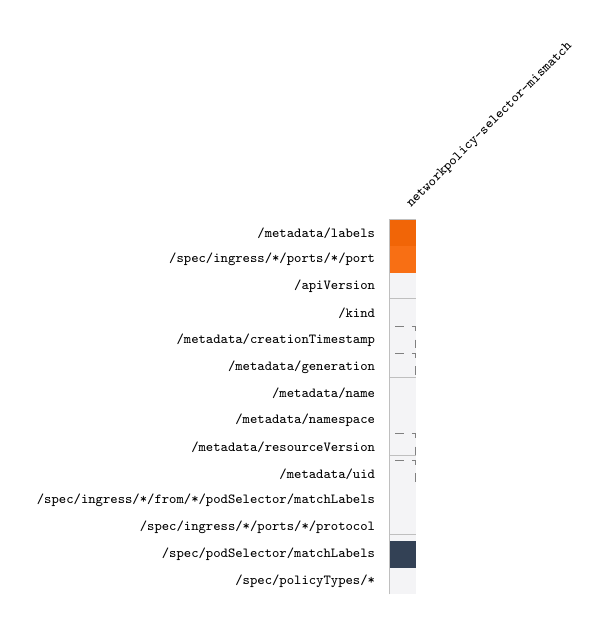
\begin{tikzpicture}[x=3.4mm,y=3.4mm]
\node[rotate=45,anchor=west,font=\ttfamily\tiny] at (0.5,0.25) {networkpolicy-selector-mismatch};
\node[anchor=east,font=\ttfamily\tiny] at (-0.15,-0.5) {/metadata/labels};
\fill[fill={rgb,255:red,241;green,101;blue,7}] (0,-1) rectangle ++(1,1);
\node[anchor=east,font=\ttfamily\tiny] at (-0.15,-1.5) {/spec/ingress/*/ports/*/port};
\fill[fill={rgb,255:red,248;green,111;blue,20}] (0,-2) rectangle ++(1,1);
\node[anchor=east,font=\ttfamily\tiny] at (-0.15,-2.5) {/apiVersion};
\fill[fill={rgb,255:red,244;green,244;blue,246}] (0,-3) rectangle ++(1,1);
\node[anchor=east,font=\ttfamily\tiny] at (-0.15,-3.5) {/kind};
\fill[fill={rgb,255:red,244;green,244;blue,246}] (0,-4) rectangle ++(1,1);
\node[anchor=east,font=\ttfamily\tiny] at (-0.15,-4.5) {/metadata/creationTimestamp};
\fill[fill={rgb,255:red,244;green,244;blue,246}] (0,-5) rectangle ++(1,1);
\draw[gray,dashed,line width=0.2pt] (0,-5) rectangle ++(1,1);
\node[anchor=east,font=\ttfamily\tiny] at (-0.15,-5.5) {/metadata/generation};
\fill[fill={rgb,255:red,244;green,244;blue,246}] (0,-6) rectangle ++(1,1);
\draw[gray,dashed,line width=0.2pt] (0,-6) rectangle ++(1,1);
\node[anchor=east,font=\ttfamily\tiny] at (-0.15,-6.5) {/metadata/name};
\fill[fill={rgb,255:red,244;green,244;blue,246}] (0,-7) rectangle ++(1,1);
\node[anchor=east,font=\ttfamily\tiny] at (-0.15,-7.5) {/metadata/namespace};
\fill[fill={rgb,255:red,244;green,244;blue,246}] (0,-8) rectangle ++(1,1);
\node[anchor=east,font=\ttfamily\tiny] at (-0.15,-8.5) {/metadata/resourceVersion};
\fill[fill={rgb,255:red,244;green,244;blue,246}] (0,-9) rectangle ++(1,1);
\draw[gray,dashed,line width=0.2pt] (0,-9) rectangle ++(1,1);
\node[anchor=east,font=\ttfamily\tiny] at (-0.15,-9.5) {/metadata/uid};
\fill[fill={rgb,255:red,244;green,244;blue,246}] (0,-10) rectangle ++(1,1);
\draw[gray,dashed,line width=0.2pt] (0,-10) rectangle ++(1,1);
\node[anchor=east,font=\ttfamily\tiny] at (-0.15,-10.5) {/spec/ingress/*/from/*/podSelector/matchLabels};
\fill[fill={rgb,255:red,244;green,244;blue,246}] (0,-11) rectangle ++(1,1);
\node[anchor=east,font=\ttfamily\tiny] at (-0.15,-11.5) {/spec/ingress/*/ports/*/protocol};
\fill[fill={rgb,255:red,244;green,244;blue,246}] (0,-12) rectangle ++(1,1);
\node[anchor=east,font=\ttfamily\tiny] at (-0.15,-12.5) {/spec/podSelector/matchLabels};
\fill[fill={rgb,255:red,51;green,65;blue,85}] (0,-13) rectangle ++(1,1);
\node[white,font=\tiny] at (0.5,-13.5) {$\ast$};
\node[anchor=east,font=\ttfamily\tiny] at (-0.15,-13.5) {/spec/policyTypes/*};
\fill[fill={rgb,255:red,244;green,244;blue,246}] (0,-14) rectangle ++(1,1);
\draw[gray!50,line width=0.2pt] (0,0) grid (1,-14);
\end{tikzpicture}

\par\medskip\noindent{\small\bfseries ServiceAccount}\par\smallskip
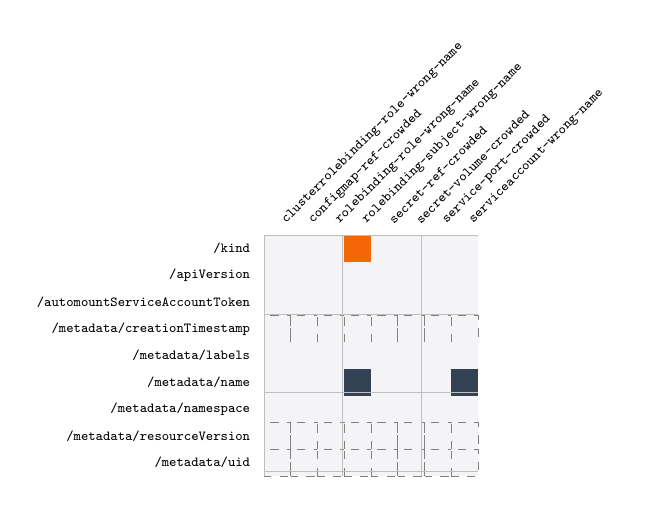
\begin{tikzpicture}[x=3.4mm,y=3.4mm]
\node[rotate=45,anchor=west,font=\ttfamily\tiny] at (0.5,0.25) {clusterrolebinding-role-wrong-name};
\node[rotate=45,anchor=west,font=\ttfamily\tiny] at (1.5,0.25) {configmap-ref-crowded};
\node[rotate=45,anchor=west,font=\ttfamily\tiny] at (2.5,0.25) {rolebinding-role-wrong-name};
\node[rotate=45,anchor=west,font=\ttfamily\tiny] at (3.5,0.25) {rolebinding-subject-wrong-name};
\node[rotate=45,anchor=west,font=\ttfamily\tiny] at (4.5,0.25) {secret-ref-crowded};
\node[rotate=45,anchor=west,font=\ttfamily\tiny] at (5.5,0.25) {secret-volume-crowded};
\node[rotate=45,anchor=west,font=\ttfamily\tiny] at (6.5,0.25) {service-port-crowded};
\node[rotate=45,anchor=west,font=\ttfamily\tiny] at (7.5,0.25) {serviceaccount-wrong-name};
\node[anchor=east,font=\ttfamily\tiny] at (-0.15,-0.5) {/kind};
\fill[fill={rgb,255:red,244;green,244;blue,246}] (0,-1) rectangle ++(1,1);
\fill[fill={rgb,255:red,244;green,244;blue,246}] (1,-1) rectangle ++(1,1);
\fill[fill={rgb,255:red,244;green,244;blue,246}] (2,-1) rectangle ++(1,1);
\fill[fill={rgb,255:red,244;green,102;blue,8}] (3,-1) rectangle ++(1,1);
\fill[fill={rgb,255:red,244;green,244;blue,246}] (4,-1) rectangle ++(1,1);
\fill[fill={rgb,255:red,244;green,244;blue,246}] (5,-1) rectangle ++(1,1);
\fill[fill={rgb,255:red,244;green,244;blue,246}] (6,-1) rectangle ++(1,1);
\fill[fill={rgb,255:red,244;green,244;blue,246}] (7,-1) rectangle ++(1,1);
\node[anchor=east,font=\ttfamily\tiny] at (-0.15,-1.5) {/apiVersion};
\fill[fill={rgb,255:red,244;green,244;blue,246}] (0,-2) rectangle ++(1,1);
\fill[fill={rgb,255:red,244;green,244;blue,246}] (1,-2) rectangle ++(1,1);
\fill[fill={rgb,255:red,244;green,244;blue,246}] (2,-2) rectangle ++(1,1);
\fill[fill={rgb,255:red,244;green,244;blue,246}] (3,-2) rectangle ++(1,1);
\fill[fill={rgb,255:red,244;green,244;blue,246}] (4,-2) rectangle ++(1,1);
\fill[fill={rgb,255:red,244;green,244;blue,246}] (5,-2) rectangle ++(1,1);
\fill[fill={rgb,255:red,244;green,244;blue,246}] (6,-2) rectangle ++(1,1);
\fill[fill={rgb,255:red,244;green,244;blue,246}] (7,-2) rectangle ++(1,1);
\node[anchor=east,font=\ttfamily\tiny] at (-0.15,-2.5) {/automountServiceAccountToken};
\fill[fill={rgb,255:red,244;green,244;blue,246}] (0,-3) rectangle ++(1,1);
\fill[fill={rgb,255:red,244;green,244;blue,246}] (1,-3) rectangle ++(1,1);
\fill[fill={rgb,255:red,244;green,244;blue,246}] (2,-3) rectangle ++(1,1);
\fill[fill={rgb,255:red,244;green,244;blue,246}] (3,-3) rectangle ++(1,1);
\fill[fill={rgb,255:red,244;green,244;blue,246}] (4,-3) rectangle ++(1,1);
\fill[fill={rgb,255:red,244;green,244;blue,246}] (5,-3) rectangle ++(1,1);
\fill[fill={rgb,255:red,244;green,244;blue,246}] (6,-3) rectangle ++(1,1);
\fill[fill={rgb,255:red,244;green,244;blue,246}] (7,-3) rectangle ++(1,1);
\node[anchor=east,font=\ttfamily\tiny] at (-0.15,-3.5) {/metadata/creationTimestamp};
\fill[fill={rgb,255:red,244;green,244;blue,246}] (0,-4) rectangle ++(1,1);
\draw[gray,dashed,line width=0.2pt] (0,-4) rectangle ++(1,1);
\fill[fill={rgb,255:red,244;green,244;blue,246}] (1,-4) rectangle ++(1,1);
\draw[gray,dashed,line width=0.2pt] (1,-4) rectangle ++(1,1);
\fill[fill={rgb,255:red,244;green,244;blue,246}] (2,-4) rectangle ++(1,1);
\draw[gray,dashed,line width=0.2pt] (2,-4) rectangle ++(1,1);
\fill[fill={rgb,255:red,244;green,244;blue,246}] (3,-4) rectangle ++(1,1);
\draw[gray,dashed,line width=0.2pt] (3,-4) rectangle ++(1,1);
\fill[fill={rgb,255:red,244;green,244;blue,246}] (4,-4) rectangle ++(1,1);
\draw[gray,dashed,line width=0.2pt] (4,-4) rectangle ++(1,1);
\fill[fill={rgb,255:red,244;green,244;blue,246}] (5,-4) rectangle ++(1,1);
\draw[gray,dashed,line width=0.2pt] (5,-4) rectangle ++(1,1);
\fill[fill={rgb,255:red,244;green,244;blue,246}] (6,-4) rectangle ++(1,1);
\draw[gray,dashed,line width=0.2pt] (6,-4) rectangle ++(1,1);
\fill[fill={rgb,255:red,244;green,244;blue,246}] (7,-4) rectangle ++(1,1);
\draw[gray,dashed,line width=0.2pt] (7,-4) rectangle ++(1,1);
\node[anchor=east,font=\ttfamily\tiny] at (-0.15,-4.5) {/metadata/labels};
\fill[fill={rgb,255:red,244;green,244;blue,246}] (0,-5) rectangle ++(1,1);
\fill[fill={rgb,255:red,244;green,244;blue,246}] (1,-5) rectangle ++(1,1);
\fill[fill={rgb,255:red,244;green,244;blue,246}] (2,-5) rectangle ++(1,1);
\fill[fill={rgb,255:red,244;green,244;blue,246}] (3,-5) rectangle ++(1,1);
\fill[fill={rgb,255:red,244;green,244;blue,246}] (4,-5) rectangle ++(1,1);
\fill[fill={rgb,255:red,244;green,244;blue,246}] (5,-5) rectangle ++(1,1);
\fill[fill={rgb,255:red,244;green,244;blue,246}] (6,-5) rectangle ++(1,1);
\fill[fill={rgb,255:red,244;green,244;blue,246}] (7,-5) rectangle ++(1,1);
\node[anchor=east,font=\ttfamily\tiny] at (-0.15,-5.5) {/metadata/name};
\fill[fill={rgb,255:red,244;green,244;blue,246}] (0,-6) rectangle ++(1,1);
\fill[fill={rgb,255:red,244;green,244;blue,246}] (1,-6) rectangle ++(1,1);
\fill[fill={rgb,255:red,244;green,244;blue,246}] (2,-6) rectangle ++(1,1);
\fill[fill={rgb,255:red,51;green,65;blue,85}] (3,-6) rectangle ++(1,1);
\node[white,font=\tiny] at (3.5,-6.5) {$\ast$};
\fill[fill={rgb,255:red,244;green,244;blue,246}] (4,-6) rectangle ++(1,1);
\fill[fill={rgb,255:red,244;green,244;blue,246}] (5,-6) rectangle ++(1,1);
\fill[fill={rgb,255:red,244;green,244;blue,246}] (6,-6) rectangle ++(1,1);
\fill[fill={rgb,255:red,51;green,65;blue,85}] (7,-6) rectangle ++(1,1);
\node[white,font=\tiny] at (7.5,-6.5) {$\ast$};
\node[anchor=east,font=\ttfamily\tiny] at (-0.15,-6.5) {/metadata/namespace};
\fill[fill={rgb,255:red,244;green,244;blue,246}] (0,-7) rectangle ++(1,1);
\fill[fill={rgb,255:red,244;green,244;blue,246}] (1,-7) rectangle ++(1,1);
\fill[fill={rgb,255:red,244;green,244;blue,246}] (2,-7) rectangle ++(1,1);
\fill[fill={rgb,255:red,244;green,244;blue,246}] (3,-7) rectangle ++(1,1);
\fill[fill={rgb,255:red,244;green,244;blue,246}] (4,-7) rectangle ++(1,1);
\fill[fill={rgb,255:red,244;green,244;blue,246}] (5,-7) rectangle ++(1,1);
\fill[fill={rgb,255:red,244;green,244;blue,246}] (6,-7) rectangle ++(1,1);
\fill[fill={rgb,255:red,244;green,244;blue,246}] (7,-7) rectangle ++(1,1);
\node[anchor=east,font=\ttfamily\tiny] at (-0.15,-7.5) {/metadata/resourceVersion};
\fill[fill={rgb,255:red,244;green,244;blue,246}] (0,-8) rectangle ++(1,1);
\draw[gray,dashed,line width=0.2pt] (0,-8) rectangle ++(1,1);
\fill[fill={rgb,255:red,244;green,244;blue,246}] (1,-8) rectangle ++(1,1);
\draw[gray,dashed,line width=0.2pt] (1,-8) rectangle ++(1,1);
\fill[fill={rgb,255:red,244;green,244;blue,246}] (2,-8) rectangle ++(1,1);
\draw[gray,dashed,line width=0.2pt] (2,-8) rectangle ++(1,1);
\fill[fill={rgb,255:red,244;green,244;blue,246}] (3,-8) rectangle ++(1,1);
\draw[gray,dashed,line width=0.2pt] (3,-8) rectangle ++(1,1);
\fill[fill={rgb,255:red,244;green,244;blue,246}] (4,-8) rectangle ++(1,1);
\draw[gray,dashed,line width=0.2pt] (4,-8) rectangle ++(1,1);
\fill[fill={rgb,255:red,244;green,244;blue,246}] (5,-8) rectangle ++(1,1);
\draw[gray,dashed,line width=0.2pt] (5,-8) rectangle ++(1,1);
\fill[fill={rgb,255:red,244;green,244;blue,246}] (6,-8) rectangle ++(1,1);
\draw[gray,dashed,line width=0.2pt] (6,-8) rectangle ++(1,1);
\fill[fill={rgb,255:red,244;green,244;blue,246}] (7,-8) rectangle ++(1,1);
\draw[gray,dashed,line width=0.2pt] (7,-8) rectangle ++(1,1);
\node[anchor=east,font=\ttfamily\tiny] at (-0.15,-8.5) {/metadata/uid};
\fill[fill={rgb,255:red,244;green,244;blue,246}] (0,-9) rectangle ++(1,1);
\draw[gray,dashed,line width=0.2pt] (0,-9) rectangle ++(1,1);
\fill[fill={rgb,255:red,244;green,244;blue,246}] (1,-9) rectangle ++(1,1);
\draw[gray,dashed,line width=0.2pt] (1,-9) rectangle ++(1,1);
\fill[fill={rgb,255:red,244;green,244;blue,246}] (2,-9) rectangle ++(1,1);
\draw[gray,dashed,line width=0.2pt] (2,-9) rectangle ++(1,1);
\fill[fill={rgb,255:red,244;green,244;blue,246}] (3,-9) rectangle ++(1,1);
\draw[gray,dashed,line width=0.2pt] (3,-9) rectangle ++(1,1);
\fill[fill={rgb,255:red,244;green,244;blue,246}] (4,-9) rectangle ++(1,1);
\draw[gray,dashed,line width=0.2pt] (4,-9) rectangle ++(1,1);
\fill[fill={rgb,255:red,244;green,244;blue,246}] (5,-9) rectangle ++(1,1);
\draw[gray,dashed,line width=0.2pt] (5,-9) rectangle ++(1,1);
\fill[fill={rgb,255:red,244;green,244;blue,246}] (6,-9) rectangle ++(1,1);
\draw[gray,dashed,line width=0.2pt] (6,-9) rectangle ++(1,1);
\fill[fill={rgb,255:red,244;green,244;blue,246}] (7,-9) rectangle ++(1,1);
\draw[gray,dashed,line width=0.2pt] (7,-9) rectangle ++(1,1);
\draw[gray!50,line width=0.2pt] (0,0) grid (8,-9);
\end{tikzpicture}

\par\medskip\noindent{\small\bfseries Secret}\par\smallskip
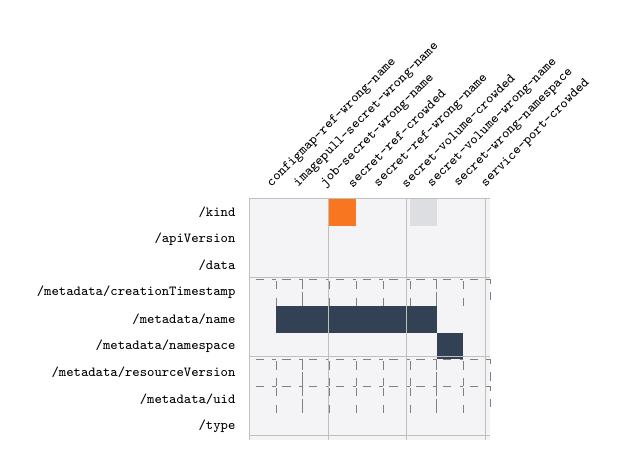
\begin{tikzpicture}[x=3.4mm,y=3.4mm]
\node[rotate=45,anchor=west,font=\ttfamily\tiny] at (0.5,0.25) {configmap-ref-wrong-name};
\node[rotate=45,anchor=west,font=\ttfamily\tiny] at (1.5,0.25) {imagepull-secret-wrong-name};
\node[rotate=45,anchor=west,font=\ttfamily\tiny] at (2.5,0.25) {job-secret-wrong-name};
\node[rotate=45,anchor=west,font=\ttfamily\tiny] at (3.5,0.25) {secret-ref-crowded};
\node[rotate=45,anchor=west,font=\ttfamily\tiny] at (4.5,0.25) {secret-ref-wrong-name};
\node[rotate=45,anchor=west,font=\ttfamily\tiny] at (5.5,0.25) {secret-volume-crowded};
\node[rotate=45,anchor=west,font=\ttfamily\tiny] at (6.5,0.25) {secret-volume-wrong-name};
\node[rotate=45,anchor=west,font=\ttfamily\tiny] at (7.5,0.25) {secret-wrong-namespace};
\node[rotate=45,anchor=west,font=\ttfamily\tiny] at (8.5,0.25) {service-port-crowded};
\node[anchor=east,font=\ttfamily\tiny] at (-0.15,-0.5) {/kind};
\fill[fill={rgb,255:red,244;green,244;blue,246}] (0,-1) rectangle ++(1,1);
\fill[fill={rgb,255:red,244;green,244;blue,246}] (1,-1) rectangle ++(1,1);
\fill[fill={rgb,255:red,244;green,244;blue,246}] (2,-1) rectangle ++(1,1);
\fill[fill={rgb,255:red,248;green,118;blue,31}] (3,-1) rectangle ++(1,1);
\fill[fill={rgb,255:red,244;green,244;blue,246}] (4,-1) rectangle ++(1,1);
\fill[fill={rgb,255:red,244;green,244;blue,246}] (5,-1) rectangle ++(1,1);
\fill[fill={rgb,255:red,221;green,222;blue,226}] (6,-1) rectangle ++(1,1);
\fill[fill={rgb,255:red,244;green,244;blue,246}] (7,-1) rectangle ++(1,1);
\fill[fill={rgb,255:red,244;green,244;blue,246}] (8,-1) rectangle ++(1,1);
\node[anchor=east,font=\ttfamily\tiny] at (-0.15,-1.5) {/apiVersion};
\fill[fill={rgb,255:red,244;green,244;blue,246}] (0,-2) rectangle ++(1,1);
\fill[fill={rgb,255:red,244;green,244;blue,246}] (1,-2) rectangle ++(1,1);
\fill[fill={rgb,255:red,244;green,244;blue,246}] (2,-2) rectangle ++(1,1);
\fill[fill={rgb,255:red,244;green,244;blue,246}] (3,-2) rectangle ++(1,1);
\fill[fill={rgb,255:red,244;green,244;blue,246}] (4,-2) rectangle ++(1,1);
\fill[fill={rgb,255:red,244;green,244;blue,246}] (5,-2) rectangle ++(1,1);
\fill[fill={rgb,255:red,244;green,244;blue,246}] (6,-2) rectangle ++(1,1);
\fill[fill={rgb,255:red,244;green,244;blue,246}] (7,-2) rectangle ++(1,1);
\fill[fill={rgb,255:red,244;green,244;blue,246}] (8,-2) rectangle ++(1,1);
\node[anchor=east,font=\ttfamily\tiny] at (-0.15,-2.5) {/data};
\fill[fill={rgb,255:red,244;green,244;blue,246}] (0,-3) rectangle ++(1,1);
\fill[fill={rgb,255:red,244;green,244;blue,246}] (1,-3) rectangle ++(1,1);
\fill[fill={rgb,255:red,244;green,244;blue,246}] (2,-3) rectangle ++(1,1);
\fill[fill={rgb,255:red,244;green,244;blue,246}] (3,-3) rectangle ++(1,1);
\fill[fill={rgb,255:red,244;green,244;blue,246}] (4,-3) rectangle ++(1,1);
\fill[fill={rgb,255:red,244;green,244;blue,246}] (5,-3) rectangle ++(1,1);
\fill[fill={rgb,255:red,244;green,244;blue,246}] (6,-3) rectangle ++(1,1);
\fill[fill={rgb,255:red,244;green,244;blue,246}] (7,-3) rectangle ++(1,1);
\fill[fill={rgb,255:red,244;green,244;blue,246}] (8,-3) rectangle ++(1,1);
\node[anchor=east,font=\ttfamily\tiny] at (-0.15,-3.5) {/metadata/creationTimestamp};
\fill[fill={rgb,255:red,244;green,244;blue,246}] (0,-4) rectangle ++(1,1);
\draw[gray,dashed,line width=0.2pt] (0,-4) rectangle ++(1,1);
\fill[fill={rgb,255:red,244;green,244;blue,246}] (1,-4) rectangle ++(1,1);
\draw[gray,dashed,line width=0.2pt] (1,-4) rectangle ++(1,1);
\fill[fill={rgb,255:red,244;green,244;blue,246}] (2,-4) rectangle ++(1,1);
\draw[gray,dashed,line width=0.2pt] (2,-4) rectangle ++(1,1);
\fill[fill={rgb,255:red,244;green,244;blue,246}] (3,-4) rectangle ++(1,1);
\draw[gray,dashed,line width=0.2pt] (3,-4) rectangle ++(1,1);
\fill[fill={rgb,255:red,244;green,244;blue,246}] (4,-4) rectangle ++(1,1);
\draw[gray,dashed,line width=0.2pt] (4,-4) rectangle ++(1,1);
\fill[fill={rgb,255:red,244;green,244;blue,246}] (5,-4) rectangle ++(1,1);
\draw[gray,dashed,line width=0.2pt] (5,-4) rectangle ++(1,1);
\fill[fill={rgb,255:red,244;green,244;blue,246}] (6,-4) rectangle ++(1,1);
\draw[gray,dashed,line width=0.2pt] (6,-4) rectangle ++(1,1);
\fill[fill={rgb,255:red,244;green,244;blue,246}] (7,-4) rectangle ++(1,1);
\draw[gray,dashed,line width=0.2pt] (7,-4) rectangle ++(1,1);
\fill[fill={rgb,255:red,244;green,244;blue,246}] (8,-4) rectangle ++(1,1);
\draw[gray,dashed,line width=0.2pt] (8,-4) rectangle ++(1,1);
\node[anchor=east,font=\ttfamily\tiny] at (-0.15,-4.5) {/metadata/name};
\fill[fill={rgb,255:red,244;green,244;blue,246}] (0,-5) rectangle ++(1,1);
\fill[fill={rgb,255:red,51;green,65;blue,85}] (1,-5) rectangle ++(1,1);
\node[white,font=\tiny] at (1.5,-5.5) {$\ast$};
\fill[fill={rgb,255:red,51;green,65;blue,85}] (2,-5) rectangle ++(1,1);
\node[white,font=\tiny] at (2.5,-5.5) {$\ast$};
\fill[fill={rgb,255:red,51;green,65;blue,85}] (3,-5) rectangle ++(1,1);
\node[white,font=\tiny] at (3.5,-5.5) {$\ast$};
\fill[fill={rgb,255:red,51;green,65;blue,85}] (4,-5) rectangle ++(1,1);
\node[white,font=\tiny] at (4.5,-5.5) {$\ast$};
\fill[fill={rgb,255:red,51;green,65;blue,85}] (5,-5) rectangle ++(1,1);
\node[white,font=\tiny] at (5.5,-5.5) {$\ast$};
\fill[fill={rgb,255:red,51;green,65;blue,85}] (6,-5) rectangle ++(1,1);
\node[white,font=\tiny] at (6.5,-5.5) {$\ast$};
\fill[fill={rgb,255:red,244;green,244;blue,246}] (7,-5) rectangle ++(1,1);
\fill[fill={rgb,255:red,244;green,244;blue,246}] (8,-5) rectangle ++(1,1);
\node[anchor=east,font=\ttfamily\tiny] at (-0.15,-5.5) {/metadata/namespace};
\fill[fill={rgb,255:red,244;green,244;blue,246}] (0,-6) rectangle ++(1,1);
\fill[fill={rgb,255:red,244;green,244;blue,246}] (1,-6) rectangle ++(1,1);
\fill[fill={rgb,255:red,244;green,244;blue,246}] (2,-6) rectangle ++(1,1);
\fill[fill={rgb,255:red,244;green,244;blue,246}] (3,-6) rectangle ++(1,1);
\fill[fill={rgb,255:red,244;green,244;blue,246}] (4,-6) rectangle ++(1,1);
\fill[fill={rgb,255:red,244;green,244;blue,246}] (5,-6) rectangle ++(1,1);
\fill[fill={rgb,255:red,244;green,244;blue,246}] (6,-6) rectangle ++(1,1);
\fill[fill={rgb,255:red,51;green,65;blue,85}] (7,-6) rectangle ++(1,1);
\node[white,font=\tiny] at (7.5,-6.5) {$\ast$};
\fill[fill={rgb,255:red,244;green,244;blue,246}] (8,-6) rectangle ++(1,1);
\node[anchor=east,font=\ttfamily\tiny] at (-0.15,-6.5) {/metadata/resourceVersion};
\fill[fill={rgb,255:red,244;green,244;blue,246}] (0,-7) rectangle ++(1,1);
\draw[gray,dashed,line width=0.2pt] (0,-7) rectangle ++(1,1);
\fill[fill={rgb,255:red,244;green,244;blue,246}] (1,-7) rectangle ++(1,1);
\draw[gray,dashed,line width=0.2pt] (1,-7) rectangle ++(1,1);
\fill[fill={rgb,255:red,244;green,244;blue,246}] (2,-7) rectangle ++(1,1);
\draw[gray,dashed,line width=0.2pt] (2,-7) rectangle ++(1,1);
\fill[fill={rgb,255:red,244;green,244;blue,246}] (3,-7) rectangle ++(1,1);
\draw[gray,dashed,line width=0.2pt] (3,-7) rectangle ++(1,1);
\fill[fill={rgb,255:red,244;green,244;blue,246}] (4,-7) rectangle ++(1,1);
\draw[gray,dashed,line width=0.2pt] (4,-7) rectangle ++(1,1);
\fill[fill={rgb,255:red,244;green,244;blue,246}] (5,-7) rectangle ++(1,1);
\draw[gray,dashed,line width=0.2pt] (5,-7) rectangle ++(1,1);
\fill[fill={rgb,255:red,244;green,244;blue,246}] (6,-7) rectangle ++(1,1);
\draw[gray,dashed,line width=0.2pt] (6,-7) rectangle ++(1,1);
\fill[fill={rgb,255:red,244;green,244;blue,246}] (7,-7) rectangle ++(1,1);
\draw[gray,dashed,line width=0.2pt] (7,-7) rectangle ++(1,1);
\fill[fill={rgb,255:red,244;green,244;blue,246}] (8,-7) rectangle ++(1,1);
\draw[gray,dashed,line width=0.2pt] (8,-7) rectangle ++(1,1);
\node[anchor=east,font=\ttfamily\tiny] at (-0.15,-7.5) {/metadata/uid};
\fill[fill={rgb,255:red,244;green,244;blue,246}] (0,-8) rectangle ++(1,1);
\draw[gray,dashed,line width=0.2pt] (0,-8) rectangle ++(1,1);
\fill[fill={rgb,255:red,244;green,244;blue,246}] (1,-8) rectangle ++(1,1);
\draw[gray,dashed,line width=0.2pt] (1,-8) rectangle ++(1,1);
\fill[fill={rgb,255:red,244;green,244;blue,246}] (2,-8) rectangle ++(1,1);
\draw[gray,dashed,line width=0.2pt] (2,-8) rectangle ++(1,1);
\fill[fill={rgb,255:red,244;green,244;blue,246}] (3,-8) rectangle ++(1,1);
\draw[gray,dashed,line width=0.2pt] (3,-8) rectangle ++(1,1);
\fill[fill={rgb,255:red,244;green,244;blue,246}] (4,-8) rectangle ++(1,1);
\draw[gray,dashed,line width=0.2pt] (4,-8) rectangle ++(1,1);
\fill[fill={rgb,255:red,244;green,244;blue,246}] (5,-8) rectangle ++(1,1);
\draw[gray,dashed,line width=0.2pt] (5,-8) rectangle ++(1,1);
\fill[fill={rgb,255:red,244;green,244;blue,246}] (6,-8) rectangle ++(1,1);
\draw[gray,dashed,line width=0.2pt] (6,-8) rectangle ++(1,1);
\fill[fill={rgb,255:red,244;green,244;blue,246}] (7,-8) rectangle ++(1,1);
\draw[gray,dashed,line width=0.2pt] (7,-8) rectangle ++(1,1);
\fill[fill={rgb,255:red,244;green,244;blue,246}] (8,-8) rectangle ++(1,1);
\draw[gray,dashed,line width=0.2pt] (8,-8) rectangle ++(1,1);
\node[anchor=east,font=\ttfamily\tiny] at (-0.15,-8.5) {/type};
\fill[fill={rgb,255:red,244;green,244;blue,246}] (0,-9) rectangle ++(1,1);
\fill[fill={rgb,255:red,244;green,244;blue,246}] (1,-9) rectangle ++(1,1);
\fill[fill={rgb,255:red,244;green,244;blue,246}] (2,-9) rectangle ++(1,1);
\fill[fill={rgb,255:red,244;green,244;blue,246}] (3,-9) rectangle ++(1,1);
\fill[fill={rgb,255:red,244;green,244;blue,246}] (4,-9) rectangle ++(1,1);
\fill[fill={rgb,255:red,244;green,244;blue,246}] (5,-9) rectangle ++(1,1);
\fill[fill={rgb,255:red,244;green,244;blue,246}] (6,-9) rectangle ++(1,1);
\fill[fill={rgb,255:red,244;green,244;blue,246}] (7,-9) rectangle ++(1,1);
\fill[fill={rgb,255:red,244;green,244;blue,246}] (8,-9) rectangle ++(1,1);
\draw[gray!50,line width=0.2pt] (0,0) grid (9,-9);
\end{tikzpicture}

\par\medskip\noindent{\small\bfseries ClusterRole}\par\smallskip
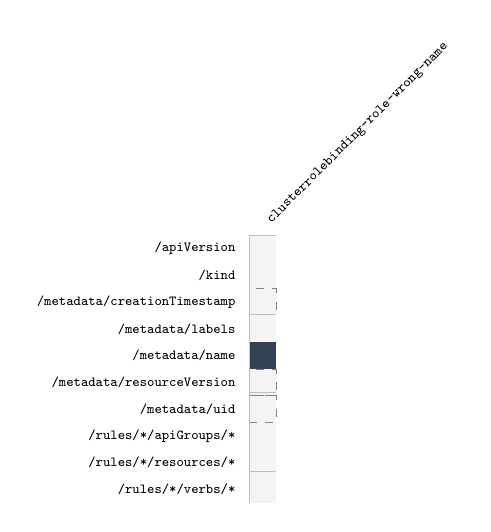
\begin{tikzpicture}[x=3.4mm,y=3.4mm]
\node[rotate=45,anchor=west,font=\ttfamily\tiny] at (0.5,0.25) {clusterrolebinding-role-wrong-name};
\node[anchor=east,font=\ttfamily\tiny] at (-0.15,-0.5) {/apiVersion};
\fill[fill={rgb,255:red,244;green,244;blue,246}] (0,-1) rectangle ++(1,1);
\node[anchor=east,font=\ttfamily\tiny] at (-0.15,-1.5) {/kind};
\fill[fill={rgb,255:red,244;green,244;blue,246}] (0,-2) rectangle ++(1,1);
\node[anchor=east,font=\ttfamily\tiny] at (-0.15,-2.5) {/metadata/creationTimestamp};
\fill[fill={rgb,255:red,244;green,244;blue,246}] (0,-3) rectangle ++(1,1);
\draw[gray,dashed,line width=0.2pt] (0,-3) rectangle ++(1,1);
\node[anchor=east,font=\ttfamily\tiny] at (-0.15,-3.5) {/metadata/labels};
\fill[fill={rgb,255:red,244;green,244;blue,246}] (0,-4) rectangle ++(1,1);
\node[anchor=east,font=\ttfamily\tiny] at (-0.15,-4.5) {/metadata/name};
\fill[fill={rgb,255:red,51;green,65;blue,85}] (0,-5) rectangle ++(1,1);
\node[white,font=\tiny] at (0.5,-5.5) {$\ast$};
\node[anchor=east,font=\ttfamily\tiny] at (-0.15,-5.5) {/metadata/resourceVersion};
\fill[fill={rgb,255:red,244;green,244;blue,246}] (0,-6) rectangle ++(1,1);
\draw[gray,dashed,line width=0.2pt] (0,-6) rectangle ++(1,1);
\node[anchor=east,font=\ttfamily\tiny] at (-0.15,-6.5) {/metadata/uid};
\fill[fill={rgb,255:red,244;green,244;blue,246}] (0,-7) rectangle ++(1,1);
\draw[gray,dashed,line width=0.2pt] (0,-7) rectangle ++(1,1);
\node[anchor=east,font=\ttfamily\tiny] at (-0.15,-7.5) {/rules/*/apiGroups/*};
\fill[fill={rgb,255:red,244;green,244;blue,246}] (0,-8) rectangle ++(1,1);
\node[anchor=east,font=\ttfamily\tiny] at (-0.15,-8.5) {/rules/*/resources/*};
\fill[fill={rgb,255:red,244;green,244;blue,246}] (0,-9) rectangle ++(1,1);
\node[anchor=east,font=\ttfamily\tiny] at (-0.15,-9.5) {/rules/*/verbs/*};
\fill[fill={rgb,255:red,244;green,244;blue,246}] (0,-10) rectangle ++(1,1);
\draw[gray!50,line width=0.2pt] (0,0) grid (1,-10);
\end{tikzpicture}

\par\medskip\noindent{\small\bfseries ClusterRoleBinding}\par\smallskip
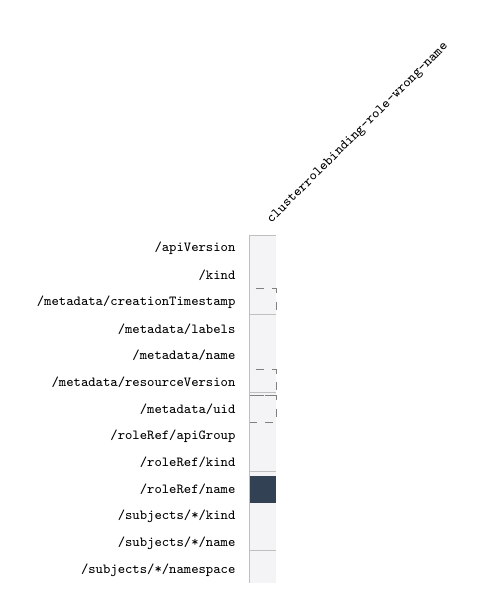
\begin{tikzpicture}[x=3.4mm,y=3.4mm]
\node[rotate=45,anchor=west,font=\ttfamily\tiny] at (0.5,0.25) {clusterrolebinding-role-wrong-name};
\node[anchor=east,font=\ttfamily\tiny] at (-0.15,-0.5) {/apiVersion};
\fill[fill={rgb,255:red,244;green,244;blue,246}] (0,-1) rectangle ++(1,1);
\node[anchor=east,font=\ttfamily\tiny] at (-0.15,-1.5) {/kind};
\fill[fill={rgb,255:red,244;green,244;blue,246}] (0,-2) rectangle ++(1,1);
\node[anchor=east,font=\ttfamily\tiny] at (-0.15,-2.5) {/metadata/creationTimestamp};
\fill[fill={rgb,255:red,244;green,244;blue,246}] (0,-3) rectangle ++(1,1);
\draw[gray,dashed,line width=0.2pt] (0,-3) rectangle ++(1,1);
\node[anchor=east,font=\ttfamily\tiny] at (-0.15,-3.5) {/metadata/labels};
\fill[fill={rgb,255:red,244;green,244;blue,246}] (0,-4) rectangle ++(1,1);
\node[anchor=east,font=\ttfamily\tiny] at (-0.15,-4.5) {/metadata/name};
\fill[fill={rgb,255:red,244;green,244;blue,246}] (0,-5) rectangle ++(1,1);
\node[anchor=east,font=\ttfamily\tiny] at (-0.15,-5.5) {/metadata/resourceVersion};
\fill[fill={rgb,255:red,244;green,244;blue,246}] (0,-6) rectangle ++(1,1);
\draw[gray,dashed,line width=0.2pt] (0,-6) rectangle ++(1,1);
\node[anchor=east,font=\ttfamily\tiny] at (-0.15,-6.5) {/metadata/uid};
\fill[fill={rgb,255:red,244;green,244;blue,246}] (0,-7) rectangle ++(1,1);
\draw[gray,dashed,line width=0.2pt] (0,-7) rectangle ++(1,1);
\node[anchor=east,font=\ttfamily\tiny] at (-0.15,-7.5) {/roleRef/apiGroup};
\fill[fill={rgb,255:red,244;green,244;blue,246}] (0,-8) rectangle ++(1,1);
\node[anchor=east,font=\ttfamily\tiny] at (-0.15,-8.5) {/roleRef/kind};
\fill[fill={rgb,255:red,244;green,244;blue,246}] (0,-9) rectangle ++(1,1);
\node[anchor=east,font=\ttfamily\tiny] at (-0.15,-9.5) {/roleRef/name};
\fill[fill={rgb,255:red,51;green,65;blue,85}] (0,-10) rectangle ++(1,1);
\node[white,font=\tiny] at (0.5,-10.5) {$\ast$};
\node[anchor=east,font=\ttfamily\tiny] at (-0.15,-10.5) {/subjects/*/kind};
\fill[fill={rgb,255:red,244;green,244;blue,246}] (0,-11) rectangle ++(1,1);
\node[anchor=east,font=\ttfamily\tiny] at (-0.15,-11.5) {/subjects/*/name};
\fill[fill={rgb,255:red,244;green,244;blue,246}] (0,-12) rectangle ++(1,1);
\node[anchor=east,font=\ttfamily\tiny] at (-0.15,-12.5) {/subjects/*/namespace};
\fill[fill={rgb,255:red,244;green,244;blue,246}] (0,-13) rectangle ++(1,1);
\draw[gray!50,line width=0.2pt] (0,0) grid (1,-13);
\end{tikzpicture}

\par\medskip\noindent{\small\bfseries DaemonSet}\par\smallskip
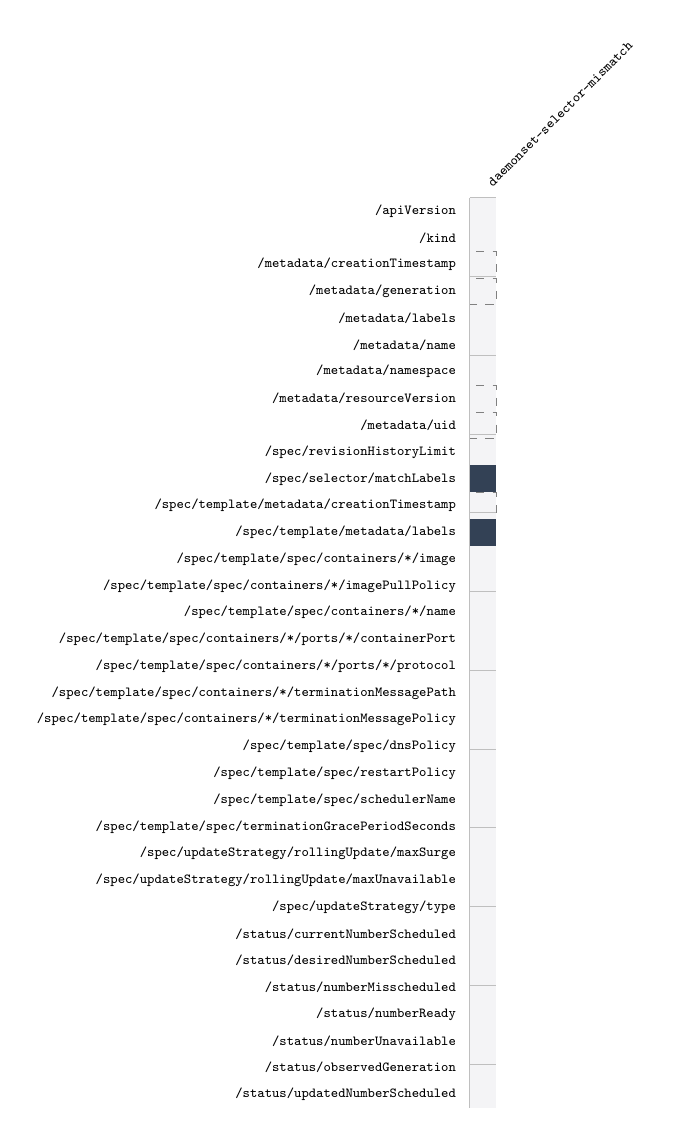
\begin{tikzpicture}[x=3.4mm,y=3.4mm]
\node[rotate=45,anchor=west,font=\ttfamily\tiny] at (0.5,0.25) {daemonset-selector-mismatch};
\node[anchor=east,font=\ttfamily\tiny] at (-0.15,-0.5) {/apiVersion};
\fill[fill={rgb,255:red,244;green,244;blue,246}] (0,-1) rectangle ++(1,1);
\node[anchor=east,font=\ttfamily\tiny] at (-0.15,-1.5) {/kind};
\fill[fill={rgb,255:red,244;green,244;blue,246}] (0,-2) rectangle ++(1,1);
\node[anchor=east,font=\ttfamily\tiny] at (-0.15,-2.5) {/metadata/creationTimestamp};
\fill[fill={rgb,255:red,244;green,244;blue,246}] (0,-3) rectangle ++(1,1);
\draw[gray,dashed,line width=0.2pt] (0,-3) rectangle ++(1,1);
\node[anchor=east,font=\ttfamily\tiny] at (-0.15,-3.5) {/metadata/generation};
\fill[fill={rgb,255:red,244;green,244;blue,246}] (0,-4) rectangle ++(1,1);
\draw[gray,dashed,line width=0.2pt] (0,-4) rectangle ++(1,1);
\node[anchor=east,font=\ttfamily\tiny] at (-0.15,-4.5) {/metadata/labels};
\fill[fill={rgb,255:red,244;green,244;blue,246}] (0,-5) rectangle ++(1,1);
\node[anchor=east,font=\ttfamily\tiny] at (-0.15,-5.5) {/metadata/name};
\fill[fill={rgb,255:red,244;green,244;blue,246}] (0,-6) rectangle ++(1,1);
\node[anchor=east,font=\ttfamily\tiny] at (-0.15,-6.5) {/metadata/namespace};
\fill[fill={rgb,255:red,244;green,244;blue,246}] (0,-7) rectangle ++(1,1);
\node[anchor=east,font=\ttfamily\tiny] at (-0.15,-7.5) {/metadata/resourceVersion};
\fill[fill={rgb,255:red,244;green,244;blue,246}] (0,-8) rectangle ++(1,1);
\draw[gray,dashed,line width=0.2pt] (0,-8) rectangle ++(1,1);
\node[anchor=east,font=\ttfamily\tiny] at (-0.15,-8.5) {/metadata/uid};
\fill[fill={rgb,255:red,244;green,244;blue,246}] (0,-9) rectangle ++(1,1);
\draw[gray,dashed,line width=0.2pt] (0,-9) rectangle ++(1,1);
\node[anchor=east,font=\ttfamily\tiny] at (-0.15,-9.5) {/spec/revisionHistoryLimit};
\fill[fill={rgb,255:red,244;green,244;blue,246}] (0,-10) rectangle ++(1,1);
\node[anchor=east,font=\ttfamily\tiny] at (-0.15,-10.5) {/spec/selector/matchLabels};
\fill[fill={rgb,255:red,51;green,65;blue,85}] (0,-11) rectangle ++(1,1);
\node[white,font=\tiny] at (0.5,-11.5) {$\ast$};
\node[anchor=east,font=\ttfamily\tiny] at (-0.15,-11.5) {/spec/template/metadata/creationTimestamp};
\fill[fill={rgb,255:red,244;green,244;blue,246}] (0,-12) rectangle ++(1,1);
\draw[gray,dashed,line width=0.2pt] (0,-12) rectangle ++(1,1);
\node[anchor=east,font=\ttfamily\tiny] at (-0.15,-12.5) {/spec/template/metadata/labels};
\fill[fill={rgb,255:red,51;green,65;blue,85}] (0,-13) rectangle ++(1,1);
\node[white,font=\tiny] at (0.5,-13.5) {$\ast$};
\node[anchor=east,font=\ttfamily\tiny] at (-0.15,-13.5) {/spec/template/spec/containers/*/image};
\fill[fill={rgb,255:red,244;green,244;blue,246}] (0,-14) rectangle ++(1,1);
\node[anchor=east,font=\ttfamily\tiny] at (-0.15,-14.5) {/spec/template/spec/containers/*/imagePullPolicy};
\fill[fill={rgb,255:red,244;green,244;blue,246}] (0,-15) rectangle ++(1,1);
\node[anchor=east,font=\ttfamily\tiny] at (-0.15,-15.5) {/spec/template/spec/containers/*/name};
\fill[fill={rgb,255:red,244;green,244;blue,246}] (0,-16) rectangle ++(1,1);
\node[anchor=east,font=\ttfamily\tiny] at (-0.15,-16.5) {/spec/template/spec/containers/*/ports/*/containerPort};
\fill[fill={rgb,255:red,244;green,244;blue,246}] (0,-17) rectangle ++(1,1);
\node[anchor=east,font=\ttfamily\tiny] at (-0.15,-17.5) {/spec/template/spec/containers/*/ports/*/protocol};
\fill[fill={rgb,255:red,244;green,244;blue,246}] (0,-18) rectangle ++(1,1);
\node[anchor=east,font=\ttfamily\tiny] at (-0.15,-18.5) {/spec/template/spec/containers/*/terminationMessagePath};
\fill[fill={rgb,255:red,244;green,244;blue,246}] (0,-19) rectangle ++(1,1);
\node[anchor=east,font=\ttfamily\tiny] at (-0.15,-19.5) {/spec/template/spec/containers/*/terminationMessagePolicy};
\fill[fill={rgb,255:red,244;green,244;blue,246}] (0,-20) rectangle ++(1,1);
\node[anchor=east,font=\ttfamily\tiny] at (-0.15,-20.5) {/spec/template/spec/dnsPolicy};
\fill[fill={rgb,255:red,244;green,244;blue,246}] (0,-21) rectangle ++(1,1);
\node[anchor=east,font=\ttfamily\tiny] at (-0.15,-21.5) {/spec/template/spec/restartPolicy};
\fill[fill={rgb,255:red,244;green,244;blue,246}] (0,-22) rectangle ++(1,1);
\node[anchor=east,font=\ttfamily\tiny] at (-0.15,-22.5) {/spec/template/spec/schedulerName};
\fill[fill={rgb,255:red,244;green,244;blue,246}] (0,-23) rectangle ++(1,1);
\node[anchor=east,font=\ttfamily\tiny] at (-0.15,-23.5) {/spec/template/spec/terminationGracePeriodSeconds};
\fill[fill={rgb,255:red,244;green,244;blue,246}] (0,-24) rectangle ++(1,1);
\node[anchor=east,font=\ttfamily\tiny] at (-0.15,-24.5) {/spec/updateStrategy/rollingUpdate/maxSurge};
\fill[fill={rgb,255:red,244;green,244;blue,246}] (0,-25) rectangle ++(1,1);
\node[anchor=east,font=\ttfamily\tiny] at (-0.15,-25.5) {/spec/updateStrategy/rollingUpdate/maxUnavailable};
\fill[fill={rgb,255:red,244;green,244;blue,246}] (0,-26) rectangle ++(1,1);
\node[anchor=east,font=\ttfamily\tiny] at (-0.15,-26.5) {/spec/updateStrategy/type};
\fill[fill={rgb,255:red,244;green,244;blue,246}] (0,-27) rectangle ++(1,1);
\node[anchor=east,font=\ttfamily\tiny] at (-0.15,-27.5) {/status/currentNumberScheduled};
\fill[fill={rgb,255:red,244;green,244;blue,246}] (0,-28) rectangle ++(1,1);
\node[anchor=east,font=\ttfamily\tiny] at (-0.15,-28.5) {/status/desiredNumberScheduled};
\fill[fill={rgb,255:red,244;green,244;blue,246}] (0,-29) rectangle ++(1,1);
\node[anchor=east,font=\ttfamily\tiny] at (-0.15,-29.5) {/status/numberMisscheduled};
\fill[fill={rgb,255:red,244;green,244;blue,246}] (0,-30) rectangle ++(1,1);
\node[anchor=east,font=\ttfamily\tiny] at (-0.15,-30.5) {/status/numberReady};
\fill[fill={rgb,255:red,244;green,244;blue,246}] (0,-31) rectangle ++(1,1);
\node[anchor=east,font=\ttfamily\tiny] at (-0.15,-31.5) {/status/numberUnavailable};
\fill[fill={rgb,255:red,244;green,244;blue,246}] (0,-32) rectangle ++(1,1);
\node[anchor=east,font=\ttfamily\tiny] at (-0.15,-32.5) {/status/observedGeneration};
\fill[fill={rgb,255:red,244;green,244;blue,246}] (0,-33) rectangle ++(1,1);
\node[anchor=east,font=\ttfamily\tiny] at (-0.15,-33.5) {/status/updatedNumberScheduled};
\fill[fill={rgb,255:red,244;green,244;blue,246}] (0,-34) rectangle ++(1,1);
\draw[gray!50,line width=0.2pt] (0,0) grid (1,-34);
\end{tikzpicture}

\par\medskip\noindent{\small\bfseries HorizontalPodAutoscaler}\par\smallskip
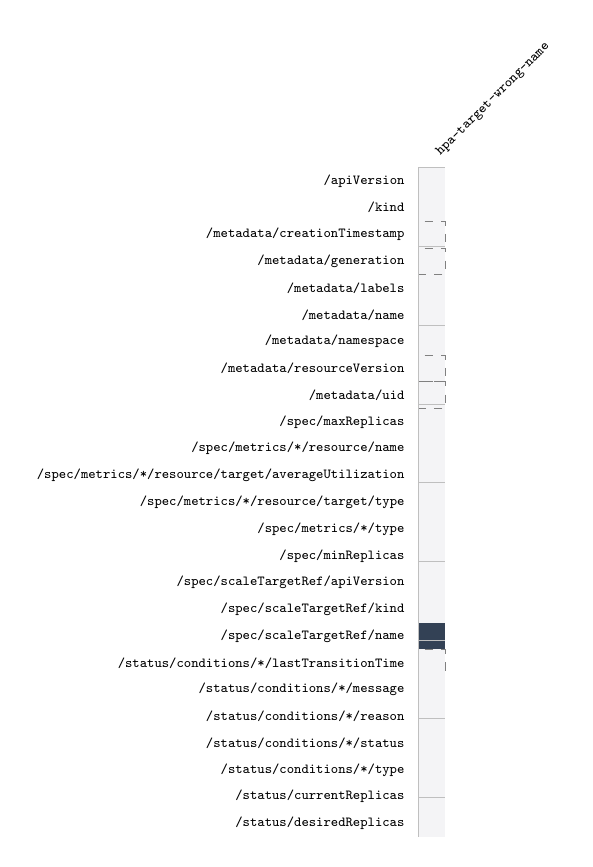
\begin{tikzpicture}[x=3.4mm,y=3.4mm]
\node[rotate=45,anchor=west,font=\ttfamily\tiny] at (0.5,0.25) {hpa-target-wrong-name};
\node[anchor=east,font=\ttfamily\tiny] at (-0.15,-0.5) {/apiVersion};
\fill[fill={rgb,255:red,244;green,244;blue,246}] (0,-1) rectangle ++(1,1);
\node[anchor=east,font=\ttfamily\tiny] at (-0.15,-1.5) {/kind};
\fill[fill={rgb,255:red,244;green,244;blue,246}] (0,-2) rectangle ++(1,1);
\node[anchor=east,font=\ttfamily\tiny] at (-0.15,-2.5) {/metadata/creationTimestamp};
\fill[fill={rgb,255:red,244;green,244;blue,246}] (0,-3) rectangle ++(1,1);
\draw[gray,dashed,line width=0.2pt] (0,-3) rectangle ++(1,1);
\node[anchor=east,font=\ttfamily\tiny] at (-0.15,-3.5) {/metadata/generation};
\fill[fill={rgb,255:red,244;green,244;blue,246}] (0,-4) rectangle ++(1,1);
\draw[gray,dashed,line width=0.2pt] (0,-4) rectangle ++(1,1);
\node[anchor=east,font=\ttfamily\tiny] at (-0.15,-4.5) {/metadata/labels};
\fill[fill={rgb,255:red,244;green,244;blue,246}] (0,-5) rectangle ++(1,1);
\node[anchor=east,font=\ttfamily\tiny] at (-0.15,-5.5) {/metadata/name};
\fill[fill={rgb,255:red,244;green,244;blue,246}] (0,-6) rectangle ++(1,1);
\node[anchor=east,font=\ttfamily\tiny] at (-0.15,-6.5) {/metadata/namespace};
\fill[fill={rgb,255:red,244;green,244;blue,246}] (0,-7) rectangle ++(1,1);
\node[anchor=east,font=\ttfamily\tiny] at (-0.15,-7.5) {/metadata/resourceVersion};
\fill[fill={rgb,255:red,244;green,244;blue,246}] (0,-8) rectangle ++(1,1);
\draw[gray,dashed,line width=0.2pt] (0,-8) rectangle ++(1,1);
\node[anchor=east,font=\ttfamily\tiny] at (-0.15,-8.5) {/metadata/uid};
\fill[fill={rgb,255:red,244;green,244;blue,246}] (0,-9) rectangle ++(1,1);
\draw[gray,dashed,line width=0.2pt] (0,-9) rectangle ++(1,1);
\node[anchor=east,font=\ttfamily\tiny] at (-0.15,-9.5) {/spec/maxReplicas};
\fill[fill={rgb,255:red,244;green,244;blue,246}] (0,-10) rectangle ++(1,1);
\node[anchor=east,font=\ttfamily\tiny] at (-0.15,-10.5) {/spec/metrics/*/resource/name};
\fill[fill={rgb,255:red,244;green,244;blue,246}] (0,-11) rectangle ++(1,1);
\node[anchor=east,font=\ttfamily\tiny] at (-0.15,-11.5) {/spec/metrics/*/resource/target/averageUtilization};
\fill[fill={rgb,255:red,244;green,244;blue,246}] (0,-12) rectangle ++(1,1);
\node[anchor=east,font=\ttfamily\tiny] at (-0.15,-12.5) {/spec/metrics/*/resource/target/type};
\fill[fill={rgb,255:red,244;green,244;blue,246}] (0,-13) rectangle ++(1,1);
\node[anchor=east,font=\ttfamily\tiny] at (-0.15,-13.5) {/spec/metrics/*/type};
\fill[fill={rgb,255:red,244;green,244;blue,246}] (0,-14) rectangle ++(1,1);
\node[anchor=east,font=\ttfamily\tiny] at (-0.15,-14.5) {/spec/minReplicas};
\fill[fill={rgb,255:red,244;green,244;blue,246}] (0,-15) rectangle ++(1,1);
\node[anchor=east,font=\ttfamily\tiny] at (-0.15,-15.5) {/spec/scaleTargetRef/apiVersion};
\fill[fill={rgb,255:red,244;green,244;blue,246}] (0,-16) rectangle ++(1,1);
\node[anchor=east,font=\ttfamily\tiny] at (-0.15,-16.5) {/spec/scaleTargetRef/kind};
\fill[fill={rgb,255:red,244;green,244;blue,246}] (0,-17) rectangle ++(1,1);
\node[anchor=east,font=\ttfamily\tiny] at (-0.15,-17.5) {/spec/scaleTargetRef/name};
\fill[fill={rgb,255:red,51;green,65;blue,85}] (0,-18) rectangle ++(1,1);
\node[white,font=\tiny] at (0.5,-18.5) {$\ast$};
\node[anchor=east,font=\ttfamily\tiny] at (-0.15,-18.5) {/status/conditions/*/lastTransitionTime};
\fill[fill={rgb,255:red,244;green,244;blue,246}] (0,-19) rectangle ++(1,1);
\draw[gray,dashed,line width=0.2pt] (0,-19) rectangle ++(1,1);
\node[anchor=east,font=\ttfamily\tiny] at (-0.15,-19.5) {/status/conditions/*/message};
\fill[fill={rgb,255:red,244;green,244;blue,246}] (0,-20) rectangle ++(1,1);
\node[anchor=east,font=\ttfamily\tiny] at (-0.15,-20.5) {/status/conditions/*/reason};
\fill[fill={rgb,255:red,244;green,244;blue,246}] (0,-21) rectangle ++(1,1);
\node[anchor=east,font=\ttfamily\tiny] at (-0.15,-21.5) {/status/conditions/*/status};
\fill[fill={rgb,255:red,244;green,244;blue,246}] (0,-22) rectangle ++(1,1);
\node[anchor=east,font=\ttfamily\tiny] at (-0.15,-22.5) {/status/conditions/*/type};
\fill[fill={rgb,255:red,244;green,244;blue,246}] (0,-23) rectangle ++(1,1);
\node[anchor=east,font=\ttfamily\tiny] at (-0.15,-23.5) {/status/currentReplicas};
\fill[fill={rgb,255:red,244;green,244;blue,246}] (0,-24) rectangle ++(1,1);
\node[anchor=east,font=\ttfamily\tiny] at (-0.15,-24.5) {/status/desiredReplicas};
\fill[fill={rgb,255:red,244;green,244;blue,246}] (0,-25) rectangle ++(1,1);
\draw[gray!50,line width=0.2pt] (0,0) grid (1,-25);
\end{tikzpicture}

\par\medskip\noindent{\small\bfseries Ingress}\par\smallskip
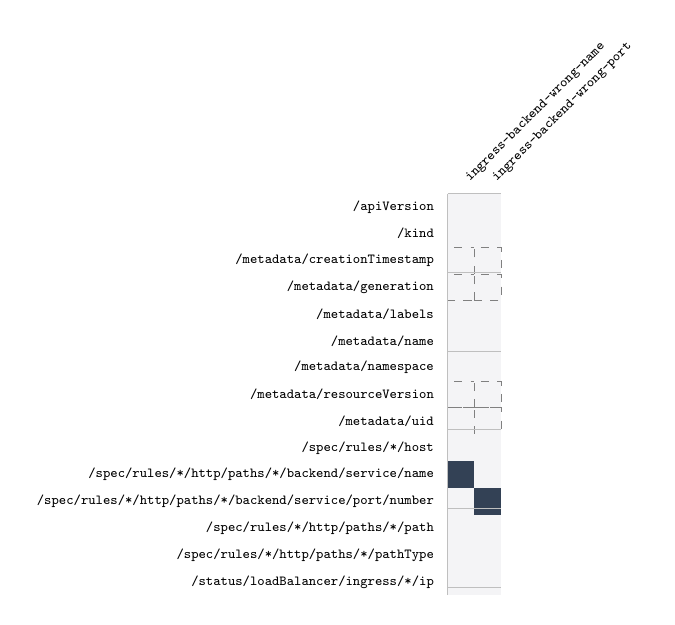
\begin{tikzpicture}[x=3.4mm,y=3.4mm]
\node[rotate=45,anchor=west,font=\ttfamily\tiny] at (0.5,0.25) {ingress-backend-wrong-name};
\node[rotate=45,anchor=west,font=\ttfamily\tiny] at (1.5,0.25) {ingress-backend-wrong-port};
\node[anchor=east,font=\ttfamily\tiny] at (-0.15,-0.5) {/apiVersion};
\fill[fill={rgb,255:red,244;green,244;blue,246}] (0,-1) rectangle ++(1,1);
\fill[fill={rgb,255:red,244;green,244;blue,246}] (1,-1) rectangle ++(1,1);
\node[anchor=east,font=\ttfamily\tiny] at (-0.15,-1.5) {/kind};
\fill[fill={rgb,255:red,244;green,244;blue,246}] (0,-2) rectangle ++(1,1);
\fill[fill={rgb,255:red,244;green,244;blue,246}] (1,-2) rectangle ++(1,1);
\node[anchor=east,font=\ttfamily\tiny] at (-0.15,-2.5) {/metadata/creationTimestamp};
\fill[fill={rgb,255:red,244;green,244;blue,246}] (0,-3) rectangle ++(1,1);
\draw[gray,dashed,line width=0.2pt] (0,-3) rectangle ++(1,1);
\fill[fill={rgb,255:red,244;green,244;blue,246}] (1,-3) rectangle ++(1,1);
\draw[gray,dashed,line width=0.2pt] (1,-3) rectangle ++(1,1);
\node[anchor=east,font=\ttfamily\tiny] at (-0.15,-3.5) {/metadata/generation};
\fill[fill={rgb,255:red,244;green,244;blue,246}] (0,-4) rectangle ++(1,1);
\draw[gray,dashed,line width=0.2pt] (0,-4) rectangle ++(1,1);
\fill[fill={rgb,255:red,244;green,244;blue,246}] (1,-4) rectangle ++(1,1);
\draw[gray,dashed,line width=0.2pt] (1,-4) rectangle ++(1,1);
\node[anchor=east,font=\ttfamily\tiny] at (-0.15,-4.5) {/metadata/labels};
\fill[fill={rgb,255:red,244;green,244;blue,246}] (0,-5) rectangle ++(1,1);
\fill[fill={rgb,255:red,244;green,244;blue,246}] (1,-5) rectangle ++(1,1);
\node[anchor=east,font=\ttfamily\tiny] at (-0.15,-5.5) {/metadata/name};
\fill[fill={rgb,255:red,244;green,244;blue,246}] (0,-6) rectangle ++(1,1);
\fill[fill={rgb,255:red,244;green,244;blue,246}] (1,-6) rectangle ++(1,1);
\node[anchor=east,font=\ttfamily\tiny] at (-0.15,-6.5) {/metadata/namespace};
\fill[fill={rgb,255:red,244;green,244;blue,246}] (0,-7) rectangle ++(1,1);
\fill[fill={rgb,255:red,244;green,244;blue,246}] (1,-7) rectangle ++(1,1);
\node[anchor=east,font=\ttfamily\tiny] at (-0.15,-7.5) {/metadata/resourceVersion};
\fill[fill={rgb,255:red,244;green,244;blue,246}] (0,-8) rectangle ++(1,1);
\draw[gray,dashed,line width=0.2pt] (0,-8) rectangle ++(1,1);
\fill[fill={rgb,255:red,244;green,244;blue,246}] (1,-8) rectangle ++(1,1);
\draw[gray,dashed,line width=0.2pt] (1,-8) rectangle ++(1,1);
\node[anchor=east,font=\ttfamily\tiny] at (-0.15,-8.5) {/metadata/uid};
\fill[fill={rgb,255:red,244;green,244;blue,246}] (0,-9) rectangle ++(1,1);
\draw[gray,dashed,line width=0.2pt] (0,-9) rectangle ++(1,1);
\fill[fill={rgb,255:red,244;green,244;blue,246}] (1,-9) rectangle ++(1,1);
\draw[gray,dashed,line width=0.2pt] (1,-9) rectangle ++(1,1);
\node[anchor=east,font=\ttfamily\tiny] at (-0.15,-9.5) {/spec/rules/*/host};
\fill[fill={rgb,255:red,244;green,244;blue,246}] (0,-10) rectangle ++(1,1);
\fill[fill={rgb,255:red,244;green,244;blue,246}] (1,-10) rectangle ++(1,1);
\node[anchor=east,font=\ttfamily\tiny] at (-0.15,-10.5) {/spec/rules/*/http/paths/*/backend/service/name};
\fill[fill={rgb,255:red,51;green,65;blue,85}] (0,-11) rectangle ++(1,1);
\node[white,font=\tiny] at (0.5,-11.5) {$\ast$};
\fill[fill={rgb,255:red,244;green,244;blue,246}] (1,-11) rectangle ++(1,1);
\node[anchor=east,font=\ttfamily\tiny] at (-0.15,-11.5) {/spec/rules/*/http/paths/*/backend/service/port/number};
\fill[fill={rgb,255:red,244;green,244;blue,246}] (0,-12) rectangle ++(1,1);
\fill[fill={rgb,255:red,51;green,65;blue,85}] (1,-12) rectangle ++(1,1);
\node[white,font=\tiny] at (1.5,-12.5) {$\ast$};
\node[anchor=east,font=\ttfamily\tiny] at (-0.15,-12.5) {/spec/rules/*/http/paths/*/path};
\fill[fill={rgb,255:red,244;green,244;blue,246}] (0,-13) rectangle ++(1,1);
\fill[fill={rgb,255:red,244;green,244;blue,246}] (1,-13) rectangle ++(1,1);
\node[anchor=east,font=\ttfamily\tiny] at (-0.15,-13.5) {/spec/rules/*/http/paths/*/pathType};
\fill[fill={rgb,255:red,244;green,244;blue,246}] (0,-14) rectangle ++(1,1);
\fill[fill={rgb,255:red,244;green,244;blue,246}] (1,-14) rectangle ++(1,1);
\node[anchor=east,font=\ttfamily\tiny] at (-0.15,-14.5) {/status/loadBalancer/ingress/*/ip};
\fill[fill={rgb,255:red,244;green,244;blue,246}] (0,-15) rectangle ++(1,1);
\fill[fill={rgb,255:red,244;green,244;blue,246}] (1,-15) rectangle ++(1,1);
\draw[gray!50,line width=0.2pt] (0,0) grid (2,-15);
\end{tikzpicture}

\par\medskip\noindent{\small\bfseries Job}\par\smallskip
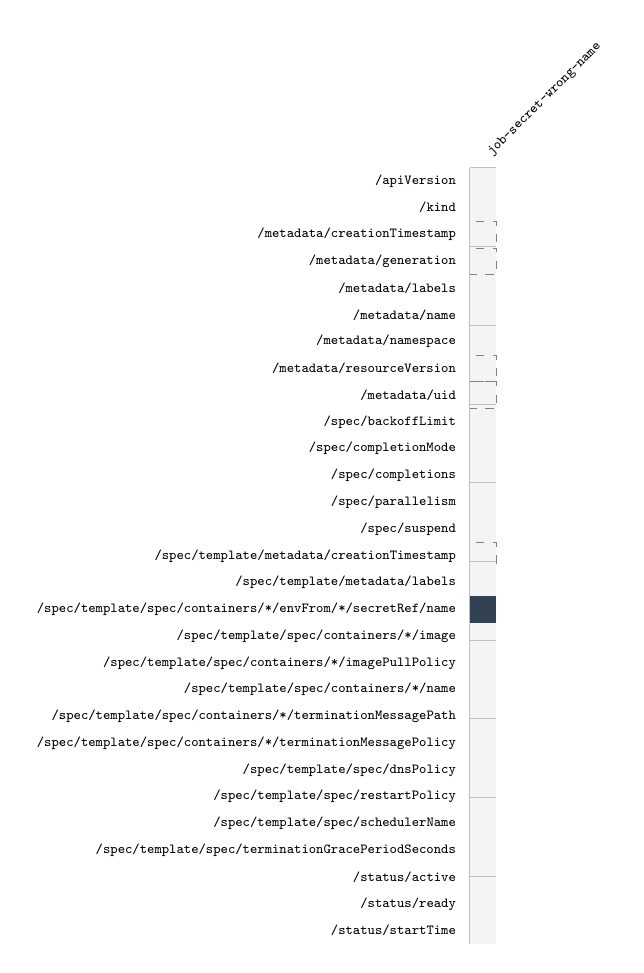
\begin{tikzpicture}[x=3.4mm,y=3.4mm]
\node[rotate=45,anchor=west,font=\ttfamily\tiny] at (0.5,0.25) {job-secret-wrong-name};
\node[anchor=east,font=\ttfamily\tiny] at (-0.15,-0.5) {/apiVersion};
\fill[fill={rgb,255:red,244;green,244;blue,246}] (0,-1) rectangle ++(1,1);
\node[anchor=east,font=\ttfamily\tiny] at (-0.15,-1.5) {/kind};
\fill[fill={rgb,255:red,244;green,244;blue,246}] (0,-2) rectangle ++(1,1);
\node[anchor=east,font=\ttfamily\tiny] at (-0.15,-2.5) {/metadata/creationTimestamp};
\fill[fill={rgb,255:red,244;green,244;blue,246}] (0,-3) rectangle ++(1,1);
\draw[gray,dashed,line width=0.2pt] (0,-3) rectangle ++(1,1);
\node[anchor=east,font=\ttfamily\tiny] at (-0.15,-3.5) {/metadata/generation};
\fill[fill={rgb,255:red,244;green,244;blue,246}] (0,-4) rectangle ++(1,1);
\draw[gray,dashed,line width=0.2pt] (0,-4) rectangle ++(1,1);
\node[anchor=east,font=\ttfamily\tiny] at (-0.15,-4.5) {/metadata/labels};
\fill[fill={rgb,255:red,244;green,244;blue,246}] (0,-5) rectangle ++(1,1);
\node[anchor=east,font=\ttfamily\tiny] at (-0.15,-5.5) {/metadata/name};
\fill[fill={rgb,255:red,244;green,244;blue,246}] (0,-6) rectangle ++(1,1);
\node[anchor=east,font=\ttfamily\tiny] at (-0.15,-6.5) {/metadata/namespace};
\fill[fill={rgb,255:red,244;green,244;blue,246}] (0,-7) rectangle ++(1,1);
\node[anchor=east,font=\ttfamily\tiny] at (-0.15,-7.5) {/metadata/resourceVersion};
\fill[fill={rgb,255:red,244;green,244;blue,246}] (0,-8) rectangle ++(1,1);
\draw[gray,dashed,line width=0.2pt] (0,-8) rectangle ++(1,1);
\node[anchor=east,font=\ttfamily\tiny] at (-0.15,-8.5) {/metadata/uid};
\fill[fill={rgb,255:red,244;green,244;blue,246}] (0,-9) rectangle ++(1,1);
\draw[gray,dashed,line width=0.2pt] (0,-9) rectangle ++(1,1);
\node[anchor=east,font=\ttfamily\tiny] at (-0.15,-9.5) {/spec/backoffLimit};
\fill[fill={rgb,255:red,244;green,244;blue,246}] (0,-10) rectangle ++(1,1);
\node[anchor=east,font=\ttfamily\tiny] at (-0.15,-10.5) {/spec/completionMode};
\fill[fill={rgb,255:red,244;green,244;blue,246}] (0,-11) rectangle ++(1,1);
\node[anchor=east,font=\ttfamily\tiny] at (-0.15,-11.5) {/spec/completions};
\fill[fill={rgb,255:red,244;green,244;blue,246}] (0,-12) rectangle ++(1,1);
\node[anchor=east,font=\ttfamily\tiny] at (-0.15,-12.5) {/spec/parallelism};
\fill[fill={rgb,255:red,244;green,244;blue,246}] (0,-13) rectangle ++(1,1);
\node[anchor=east,font=\ttfamily\tiny] at (-0.15,-13.5) {/spec/suspend};
\fill[fill={rgb,255:red,244;green,244;blue,246}] (0,-14) rectangle ++(1,1);
\node[anchor=east,font=\ttfamily\tiny] at (-0.15,-14.5) {/spec/template/metadata/creationTimestamp};
\fill[fill={rgb,255:red,244;green,244;blue,246}] (0,-15) rectangle ++(1,1);
\draw[gray,dashed,line width=0.2pt] (0,-15) rectangle ++(1,1);
\node[anchor=east,font=\ttfamily\tiny] at (-0.15,-15.5) {/spec/template/metadata/labels};
\fill[fill={rgb,255:red,244;green,244;blue,246}] (0,-16) rectangle ++(1,1);
\node[anchor=east,font=\ttfamily\tiny] at (-0.15,-16.5) {/spec/template/spec/containers/*/envFrom/*/secretRef/name};
\fill[fill={rgb,255:red,51;green,65;blue,85}] (0,-17) rectangle ++(1,1);
\node[white,font=\tiny] at (0.5,-17.5) {$\ast$};
\node[anchor=east,font=\ttfamily\tiny] at (-0.15,-17.5) {/spec/template/spec/containers/*/image};
\fill[fill={rgb,255:red,244;green,244;blue,246}] (0,-18) rectangle ++(1,1);
\node[anchor=east,font=\ttfamily\tiny] at (-0.15,-18.5) {/spec/template/spec/containers/*/imagePullPolicy};
\fill[fill={rgb,255:red,244;green,244;blue,246}] (0,-19) rectangle ++(1,1);
\node[anchor=east,font=\ttfamily\tiny] at (-0.15,-19.5) {/spec/template/spec/containers/*/name};
\fill[fill={rgb,255:red,244;green,244;blue,246}] (0,-20) rectangle ++(1,1);
\node[anchor=east,font=\ttfamily\tiny] at (-0.15,-20.5) {/spec/template/spec/containers/*/terminationMessagePath};
\fill[fill={rgb,255:red,244;green,244;blue,246}] (0,-21) rectangle ++(1,1);
\node[anchor=east,font=\ttfamily\tiny] at (-0.15,-21.5) {/spec/template/spec/containers/*/terminationMessagePolicy};
\fill[fill={rgb,255:red,244;green,244;blue,246}] (0,-22) rectangle ++(1,1);
\node[anchor=east,font=\ttfamily\tiny] at (-0.15,-22.5) {/spec/template/spec/dnsPolicy};
\fill[fill={rgb,255:red,244;green,244;blue,246}] (0,-23) rectangle ++(1,1);
\node[anchor=east,font=\ttfamily\tiny] at (-0.15,-23.5) {/spec/template/spec/restartPolicy};
\fill[fill={rgb,255:red,244;green,244;blue,246}] (0,-24) rectangle ++(1,1);
\node[anchor=east,font=\ttfamily\tiny] at (-0.15,-24.5) {/spec/template/spec/schedulerName};
\fill[fill={rgb,255:red,244;green,244;blue,246}] (0,-25) rectangle ++(1,1);
\node[anchor=east,font=\ttfamily\tiny] at (-0.15,-25.5) {/spec/template/spec/terminationGracePeriodSeconds};
\fill[fill={rgb,255:red,244;green,244;blue,246}] (0,-26) rectangle ++(1,1);
\node[anchor=east,font=\ttfamily\tiny] at (-0.15,-26.5) {/status/active};
\fill[fill={rgb,255:red,244;green,244;blue,246}] (0,-27) rectangle ++(1,1);
\node[anchor=east,font=\ttfamily\tiny] at (-0.15,-27.5) {/status/ready};
\fill[fill={rgb,255:red,244;green,244;blue,246}] (0,-28) rectangle ++(1,1);
\node[anchor=east,font=\ttfamily\tiny] at (-0.15,-28.5) {/status/startTime};
\fill[fill={rgb,255:red,244;green,244;blue,246}] (0,-29) rectangle ++(1,1);
\draw[gray!50,line width=0.2pt] (0,0) grid (1,-29);
\end{tikzpicture}

\par\medskip\noindent{\small\bfseries PriorityClass}\par\smallskip
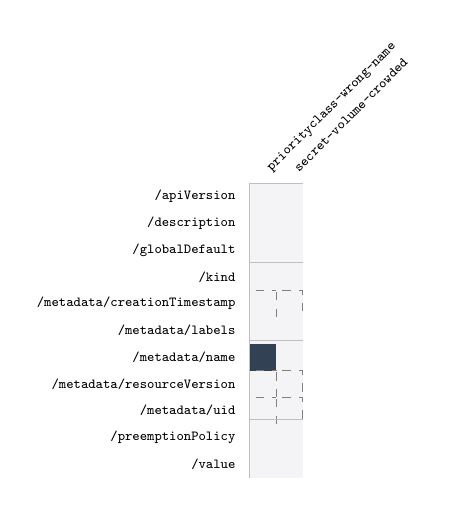
\begin{tikzpicture}[x=3.4mm,y=3.4mm]
\node[rotate=45,anchor=west,font=\ttfamily\tiny] at (0.5,0.25) {priorityclass-wrong-name};
\node[rotate=45,anchor=west,font=\ttfamily\tiny] at (1.5,0.25) {secret-volume-crowded};
\node[anchor=east,font=\ttfamily\tiny] at (-0.15,-0.5) {/apiVersion};
\fill[fill={rgb,255:red,244;green,244;blue,246}] (0,-1) rectangle ++(1,1);
\fill[fill={rgb,255:red,244;green,244;blue,246}] (1,-1) rectangle ++(1,1);
\node[anchor=east,font=\ttfamily\tiny] at (-0.15,-1.5) {/description};
\fill[fill={rgb,255:red,244;green,244;blue,246}] (0,-2) rectangle ++(1,1);
\fill[fill={rgb,255:red,244;green,244;blue,246}] (1,-2) rectangle ++(1,1);
\node[anchor=east,font=\ttfamily\tiny] at (-0.15,-2.5) {/globalDefault};
\fill[fill={rgb,255:red,244;green,244;blue,246}] (0,-3) rectangle ++(1,1);
\fill[fill={rgb,255:red,244;green,244;blue,246}] (1,-3) rectangle ++(1,1);
\node[anchor=east,font=\ttfamily\tiny] at (-0.15,-3.5) {/kind};
\fill[fill={rgb,255:red,244;green,244;blue,246}] (0,-4) rectangle ++(1,1);
\fill[fill={rgb,255:red,244;green,244;blue,246}] (1,-4) rectangle ++(1,1);
\node[anchor=east,font=\ttfamily\tiny] at (-0.15,-4.5) {/metadata/creationTimestamp};
\fill[fill={rgb,255:red,244;green,244;blue,246}] (0,-5) rectangle ++(1,1);
\draw[gray,dashed,line width=0.2pt] (0,-5) rectangle ++(1,1);
\fill[fill={rgb,255:red,244;green,244;blue,246}] (1,-5) rectangle ++(1,1);
\draw[gray,dashed,line width=0.2pt] (1,-5) rectangle ++(1,1);
\node[anchor=east,font=\ttfamily\tiny] at (-0.15,-5.5) {/metadata/labels};
\fill[fill={rgb,255:red,244;green,244;blue,246}] (0,-6) rectangle ++(1,1);
\fill[fill={rgb,255:red,244;green,244;blue,246}] (1,-6) rectangle ++(1,1);
\node[anchor=east,font=\ttfamily\tiny] at (-0.15,-6.5) {/metadata/name};
\fill[fill={rgb,255:red,51;green,65;blue,85}] (0,-7) rectangle ++(1,1);
\node[white,font=\tiny] at (0.5,-7.5) {$\ast$};
\fill[fill={rgb,255:red,244;green,244;blue,246}] (1,-7) rectangle ++(1,1);
\node[anchor=east,font=\ttfamily\tiny] at (-0.15,-7.5) {/metadata/resourceVersion};
\fill[fill={rgb,255:red,244;green,244;blue,246}] (0,-8) rectangle ++(1,1);
\draw[gray,dashed,line width=0.2pt] (0,-8) rectangle ++(1,1);
\fill[fill={rgb,255:red,244;green,244;blue,246}] (1,-8) rectangle ++(1,1);
\draw[gray,dashed,line width=0.2pt] (1,-8) rectangle ++(1,1);
\node[anchor=east,font=\ttfamily\tiny] at (-0.15,-8.5) {/metadata/uid};
\fill[fill={rgb,255:red,244;green,244;blue,246}] (0,-9) rectangle ++(1,1);
\draw[gray,dashed,line width=0.2pt] (0,-9) rectangle ++(1,1);
\fill[fill={rgb,255:red,244;green,244;blue,246}] (1,-9) rectangle ++(1,1);
\draw[gray,dashed,line width=0.2pt] (1,-9) rectangle ++(1,1);
\node[anchor=east,font=\ttfamily\tiny] at (-0.15,-9.5) {/preemptionPolicy};
\fill[fill={rgb,255:red,244;green,244;blue,246}] (0,-10) rectangle ++(1,1);
\fill[fill={rgb,255:red,244;green,244;blue,246}] (1,-10) rectangle ++(1,1);
\node[anchor=east,font=\ttfamily\tiny] at (-0.15,-10.5) {/value};
\fill[fill={rgb,255:red,244;green,244;blue,246}] (0,-11) rectangle ++(1,1);
\fill[fill={rgb,255:red,244;green,244;blue,246}] (1,-11) rectangle ++(1,1);
\draw[gray!50,line width=0.2pt] (0,0) grid (2,-11);
\end{tikzpicture}

\par\medskip\noindent{\small\bfseries ReplicaSet}\par\smallskip
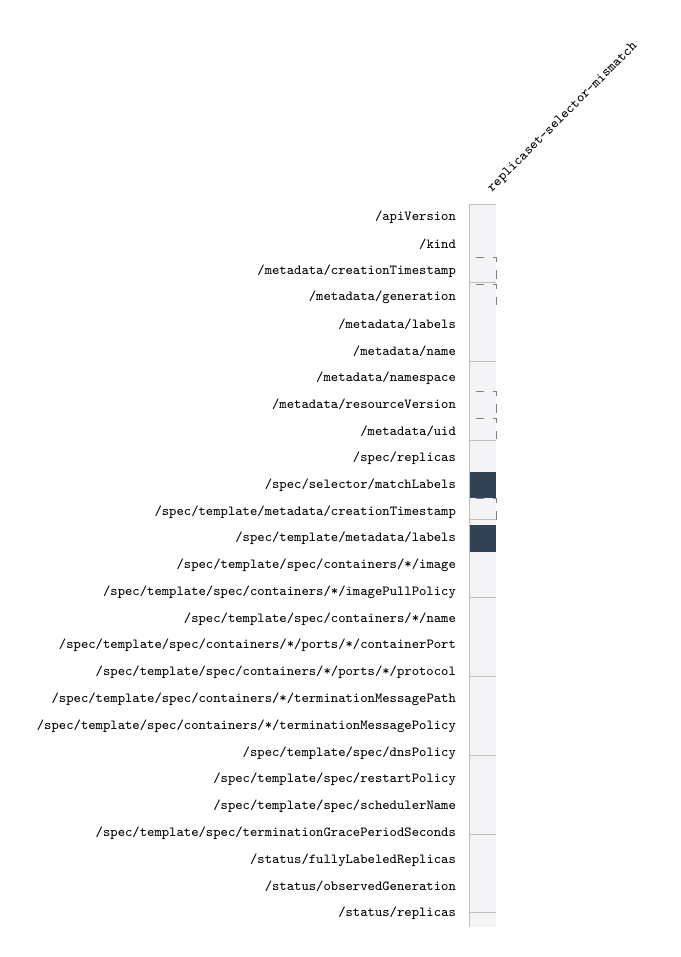
\begin{tikzpicture}[x=3.4mm,y=3.4mm]
\node[rotate=45,anchor=west,font=\ttfamily\tiny] at (0.5,0.25) {replicaset-selector-mismatch};
\node[anchor=east,font=\ttfamily\tiny] at (-0.15,-0.5) {/apiVersion};
\fill[fill={rgb,255:red,244;green,244;blue,246}] (0,-1) rectangle ++(1,1);
\node[anchor=east,font=\ttfamily\tiny] at (-0.15,-1.5) {/kind};
\fill[fill={rgb,255:red,244;green,244;blue,246}] (0,-2) rectangle ++(1,1);
\node[anchor=east,font=\ttfamily\tiny] at (-0.15,-2.5) {/metadata/creationTimestamp};
\fill[fill={rgb,255:red,244;green,244;blue,246}] (0,-3) rectangle ++(1,1);
\draw[gray,dashed,line width=0.2pt] (0,-3) rectangle ++(1,1);
\node[anchor=east,font=\ttfamily\tiny] at (-0.15,-3.5) {/metadata/generation};
\fill[fill={rgb,255:red,244;green,244;blue,246}] (0,-4) rectangle ++(1,1);
\draw[gray,dashed,line width=0.2pt] (0,-4) rectangle ++(1,1);
\node[anchor=east,font=\ttfamily\tiny] at (-0.15,-4.5) {/metadata/labels};
\fill[fill={rgb,255:red,244;green,244;blue,246}] (0,-5) rectangle ++(1,1);
\node[anchor=east,font=\ttfamily\tiny] at (-0.15,-5.5) {/metadata/name};
\fill[fill={rgb,255:red,244;green,244;blue,246}] (0,-6) rectangle ++(1,1);
\node[anchor=east,font=\ttfamily\tiny] at (-0.15,-6.5) {/metadata/namespace};
\fill[fill={rgb,255:red,244;green,244;blue,246}] (0,-7) rectangle ++(1,1);
\node[anchor=east,font=\ttfamily\tiny] at (-0.15,-7.5) {/metadata/resourceVersion};
\fill[fill={rgb,255:red,244;green,244;blue,246}] (0,-8) rectangle ++(1,1);
\draw[gray,dashed,line width=0.2pt] (0,-8) rectangle ++(1,1);
\node[anchor=east,font=\ttfamily\tiny] at (-0.15,-8.5) {/metadata/uid};
\fill[fill={rgb,255:red,244;green,244;blue,246}] (0,-9) rectangle ++(1,1);
\draw[gray,dashed,line width=0.2pt] (0,-9) rectangle ++(1,1);
\node[anchor=east,font=\ttfamily\tiny] at (-0.15,-9.5) {/spec/replicas};
\fill[fill={rgb,255:red,244;green,244;blue,246}] (0,-10) rectangle ++(1,1);
\node[anchor=east,font=\ttfamily\tiny] at (-0.15,-10.5) {/spec/selector/matchLabels};
\fill[fill={rgb,255:red,51;green,65;blue,85}] (0,-11) rectangle ++(1,1);
\node[white,font=\tiny] at (0.5,-11.5) {$\ast$};
\node[anchor=east,font=\ttfamily\tiny] at (-0.15,-11.5) {/spec/template/metadata/creationTimestamp};
\fill[fill={rgb,255:red,244;green,244;blue,246}] (0,-12) rectangle ++(1,1);
\draw[gray,dashed,line width=0.2pt] (0,-12) rectangle ++(1,1);
\node[anchor=east,font=\ttfamily\tiny] at (-0.15,-12.5) {/spec/template/metadata/labels};
\fill[fill={rgb,255:red,51;green,65;blue,85}] (0,-13) rectangle ++(1,1);
\node[white,font=\tiny] at (0.5,-13.5) {$\ast$};
\node[anchor=east,font=\ttfamily\tiny] at (-0.15,-13.5) {/spec/template/spec/containers/*/image};
\fill[fill={rgb,255:red,244;green,244;blue,246}] (0,-14) rectangle ++(1,1);
\node[anchor=east,font=\ttfamily\tiny] at (-0.15,-14.5) {/spec/template/spec/containers/*/imagePullPolicy};
\fill[fill={rgb,255:red,244;green,244;blue,246}] (0,-15) rectangle ++(1,1);
\node[anchor=east,font=\ttfamily\tiny] at (-0.15,-15.5) {/spec/template/spec/containers/*/name};
\fill[fill={rgb,255:red,244;green,244;blue,246}] (0,-16) rectangle ++(1,1);
\node[anchor=east,font=\ttfamily\tiny] at (-0.15,-16.5) {/spec/template/spec/containers/*/ports/*/containerPort};
\fill[fill={rgb,255:red,244;green,244;blue,246}] (0,-17) rectangle ++(1,1);
\node[anchor=east,font=\ttfamily\tiny] at (-0.15,-17.5) {/spec/template/spec/containers/*/ports/*/protocol};
\fill[fill={rgb,255:red,244;green,244;blue,246}] (0,-18) rectangle ++(1,1);
\node[anchor=east,font=\ttfamily\tiny] at (-0.15,-18.5) {/spec/template/spec/containers/*/terminationMessagePath};
\fill[fill={rgb,255:red,244;green,244;blue,246}] (0,-19) rectangle ++(1,1);
\node[anchor=east,font=\ttfamily\tiny] at (-0.15,-19.5) {/spec/template/spec/containers/*/terminationMessagePolicy};
\fill[fill={rgb,255:red,244;green,244;blue,246}] (0,-20) rectangle ++(1,1);
\node[anchor=east,font=\ttfamily\tiny] at (-0.15,-20.5) {/spec/template/spec/dnsPolicy};
\fill[fill={rgb,255:red,244;green,244;blue,246}] (0,-21) rectangle ++(1,1);
\node[anchor=east,font=\ttfamily\tiny] at (-0.15,-21.5) {/spec/template/spec/restartPolicy};
\fill[fill={rgb,255:red,244;green,244;blue,246}] (0,-22) rectangle ++(1,1);
\node[anchor=east,font=\ttfamily\tiny] at (-0.15,-22.5) {/spec/template/spec/schedulerName};
\fill[fill={rgb,255:red,244;green,244;blue,246}] (0,-23) rectangle ++(1,1);
\node[anchor=east,font=\ttfamily\tiny] at (-0.15,-23.5) {/spec/template/spec/terminationGracePeriodSeconds};
\fill[fill={rgb,255:red,244;green,244;blue,246}] (0,-24) rectangle ++(1,1);
\node[anchor=east,font=\ttfamily\tiny] at (-0.15,-24.5) {/status/fullyLabeledReplicas};
\fill[fill={rgb,255:red,244;green,244;blue,246}] (0,-25) rectangle ++(1,1);
\node[anchor=east,font=\ttfamily\tiny] at (-0.15,-25.5) {/status/observedGeneration};
\fill[fill={rgb,255:red,244;green,244;blue,246}] (0,-26) rectangle ++(1,1);
\node[anchor=east,font=\ttfamily\tiny] at (-0.15,-26.5) {/status/replicas};
\fill[fill={rgb,255:red,244;green,244;blue,246}] (0,-27) rectangle ++(1,1);
\draw[gray!50,line width=0.2pt] (0,0) grid (1,-27);
\end{tikzpicture}

\par\medskip\noindent{\small\bfseries RoleBinding}\par\smallskip
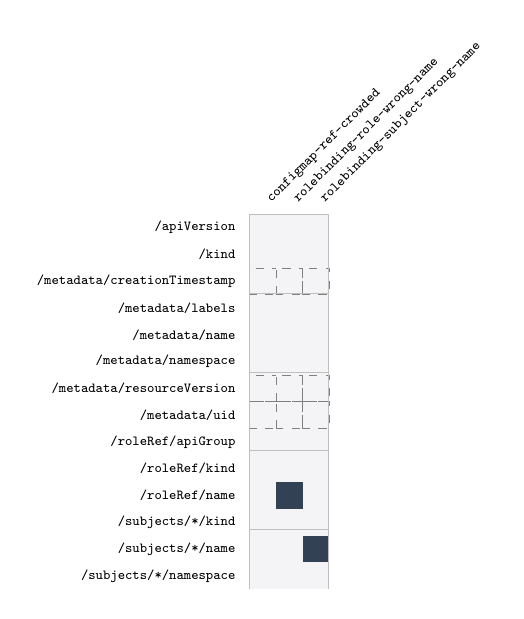
\begin{tikzpicture}[x=3.4mm,y=3.4mm]
\node[rotate=45,anchor=west,font=\ttfamily\tiny] at (0.5,0.25) {configmap-ref-crowded};
\node[rotate=45,anchor=west,font=\ttfamily\tiny] at (1.5,0.25) {rolebinding-role-wrong-name};
\node[rotate=45,anchor=west,font=\ttfamily\tiny] at (2.5,0.25) {rolebinding-subject-wrong-name};
\node[anchor=east,font=\ttfamily\tiny] at (-0.15,-0.5) {/apiVersion};
\fill[fill={rgb,255:red,244;green,244;blue,246}] (0,-1) rectangle ++(1,1);
\fill[fill={rgb,255:red,244;green,244;blue,246}] (1,-1) rectangle ++(1,1);
\fill[fill={rgb,255:red,244;green,244;blue,246}] (2,-1) rectangle ++(1,1);
\node[anchor=east,font=\ttfamily\tiny] at (-0.15,-1.5) {/kind};
\fill[fill={rgb,255:red,244;green,244;blue,246}] (0,-2) rectangle ++(1,1);
\fill[fill={rgb,255:red,244;green,244;blue,246}] (1,-2) rectangle ++(1,1);
\fill[fill={rgb,255:red,244;green,244;blue,246}] (2,-2) rectangle ++(1,1);
\node[anchor=east,font=\ttfamily\tiny] at (-0.15,-2.5) {/metadata/creationTimestamp};
\fill[fill={rgb,255:red,244;green,244;blue,246}] (0,-3) rectangle ++(1,1);
\draw[gray,dashed,line width=0.2pt] (0,-3) rectangle ++(1,1);
\fill[fill={rgb,255:red,244;green,244;blue,246}] (1,-3) rectangle ++(1,1);
\draw[gray,dashed,line width=0.2pt] (1,-3) rectangle ++(1,1);
\fill[fill={rgb,255:red,244;green,244;blue,246}] (2,-3) rectangle ++(1,1);
\draw[gray,dashed,line width=0.2pt] (2,-3) rectangle ++(1,1);
\node[anchor=east,font=\ttfamily\tiny] at (-0.15,-3.5) {/metadata/labels};
\fill[fill={rgb,255:red,244;green,244;blue,246}] (0,-4) rectangle ++(1,1);
\fill[fill={rgb,255:red,244;green,244;blue,246}] (1,-4) rectangle ++(1,1);
\fill[fill={rgb,255:red,244;green,244;blue,246}] (2,-4) rectangle ++(1,1);
\node[anchor=east,font=\ttfamily\tiny] at (-0.15,-4.5) {/metadata/name};
\fill[fill={rgb,255:red,244;green,244;blue,246}] (0,-5) rectangle ++(1,1);
\fill[fill={rgb,255:red,244;green,244;blue,246}] (1,-5) rectangle ++(1,1);
\fill[fill={rgb,255:red,244;green,244;blue,246}] (2,-5) rectangle ++(1,1);
\node[anchor=east,font=\ttfamily\tiny] at (-0.15,-5.5) {/metadata/namespace};
\fill[fill={rgb,255:red,244;green,244;blue,246}] (0,-6) rectangle ++(1,1);
\fill[fill={rgb,255:red,244;green,244;blue,246}] (1,-6) rectangle ++(1,1);
\fill[fill={rgb,255:red,244;green,244;blue,246}] (2,-6) rectangle ++(1,1);
\node[anchor=east,font=\ttfamily\tiny] at (-0.15,-6.5) {/metadata/resourceVersion};
\fill[fill={rgb,255:red,244;green,244;blue,246}] (0,-7) rectangle ++(1,1);
\draw[gray,dashed,line width=0.2pt] (0,-7) rectangle ++(1,1);
\fill[fill={rgb,255:red,244;green,244;blue,246}] (1,-7) rectangle ++(1,1);
\draw[gray,dashed,line width=0.2pt] (1,-7) rectangle ++(1,1);
\fill[fill={rgb,255:red,244;green,244;blue,246}] (2,-7) rectangle ++(1,1);
\draw[gray,dashed,line width=0.2pt] (2,-7) rectangle ++(1,1);
\node[anchor=east,font=\ttfamily\tiny] at (-0.15,-7.5) {/metadata/uid};
\fill[fill={rgb,255:red,244;green,244;blue,246}] (0,-8) rectangle ++(1,1);
\draw[gray,dashed,line width=0.2pt] (0,-8) rectangle ++(1,1);
\fill[fill={rgb,255:red,244;green,244;blue,246}] (1,-8) rectangle ++(1,1);
\draw[gray,dashed,line width=0.2pt] (1,-8) rectangle ++(1,1);
\fill[fill={rgb,255:red,244;green,244;blue,246}] (2,-8) rectangle ++(1,1);
\draw[gray,dashed,line width=0.2pt] (2,-8) rectangle ++(1,1);
\node[anchor=east,font=\ttfamily\tiny] at (-0.15,-8.5) {/roleRef/apiGroup};
\fill[fill={rgb,255:red,244;green,244;blue,246}] (0,-9) rectangle ++(1,1);
\fill[fill={rgb,255:red,244;green,244;blue,246}] (1,-9) rectangle ++(1,1);
\fill[fill={rgb,255:red,244;green,244;blue,246}] (2,-9) rectangle ++(1,1);
\node[anchor=east,font=\ttfamily\tiny] at (-0.15,-9.5) {/roleRef/kind};
\fill[fill={rgb,255:red,244;green,244;blue,246}] (0,-10) rectangle ++(1,1);
\fill[fill={rgb,255:red,244;green,244;blue,246}] (1,-10) rectangle ++(1,1);
\fill[fill={rgb,255:red,244;green,244;blue,246}] (2,-10) rectangle ++(1,1);
\node[anchor=east,font=\ttfamily\tiny] at (-0.15,-10.5) {/roleRef/name};
\fill[fill={rgb,255:red,244;green,244;blue,246}] (0,-11) rectangle ++(1,1);
\fill[fill={rgb,255:red,51;green,65;blue,85}] (1,-11) rectangle ++(1,1);
\node[white,font=\tiny] at (1.5,-11.5) {$\ast$};
\fill[fill={rgb,255:red,244;green,244;blue,246}] (2,-11) rectangle ++(1,1);
\node[anchor=east,font=\ttfamily\tiny] at (-0.15,-11.5) {/subjects/*/kind};
\fill[fill={rgb,255:red,244;green,244;blue,246}] (0,-12) rectangle ++(1,1);
\fill[fill={rgb,255:red,244;green,244;blue,246}] (1,-12) rectangle ++(1,1);
\fill[fill={rgb,255:red,244;green,244;blue,246}] (2,-12) rectangle ++(1,1);
\node[anchor=east,font=\ttfamily\tiny] at (-0.15,-12.5) {/subjects/*/name};
\fill[fill={rgb,255:red,244;green,244;blue,246}] (0,-13) rectangle ++(1,1);
\fill[fill={rgb,255:red,244;green,244;blue,246}] (1,-13) rectangle ++(1,1);
\fill[fill={rgb,255:red,51;green,65;blue,85}] (2,-13) rectangle ++(1,1);
\node[white,font=\tiny] at (2.5,-13.5) {$\ast$};
\node[anchor=east,font=\ttfamily\tiny] at (-0.15,-13.5) {/subjects/*/namespace};
\fill[fill={rgb,255:red,244;green,244;blue,246}] (0,-14) rectangle ++(1,1);
\fill[fill={rgb,255:red,244;green,244;blue,246}] (1,-14) rectangle ++(1,1);
\fill[fill={rgb,255:red,244;green,244;blue,246}] (2,-14) rectangle ++(1,1);
\draw[gray!50,line width=0.2pt] (0,0) grid (3,-14);
\end{tikzpicture}

\par\medskip\noindent{\small\bfseries Service}\par\smallskip
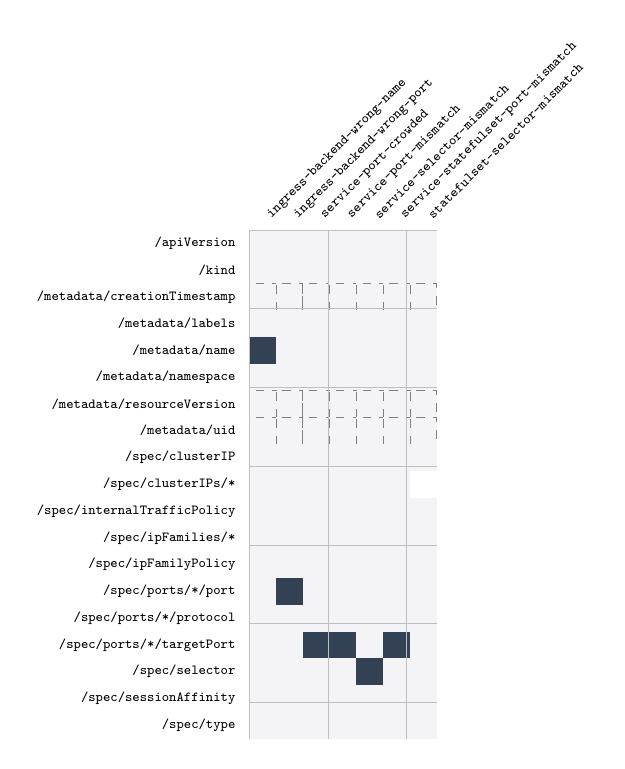
\begin{tikzpicture}[x=3.4mm,y=3.4mm]
\node[rotate=45,anchor=west,font=\ttfamily\tiny] at (0.5,0.25) {ingress-backend-wrong-name};
\node[rotate=45,anchor=west,font=\ttfamily\tiny] at (1.5,0.25) {ingress-backend-wrong-port};
\node[rotate=45,anchor=west,font=\ttfamily\tiny] at (2.5,0.25) {service-port-crowded};
\node[rotate=45,anchor=west,font=\ttfamily\tiny] at (3.5,0.25) {service-port-mismatch};
\node[rotate=45,anchor=west,font=\ttfamily\tiny] at (4.5,0.25) {service-selector-mismatch};
\node[rotate=45,anchor=west,font=\ttfamily\tiny] at (5.5,0.25) {service-statefulset-port-mismatch};
\node[rotate=45,anchor=west,font=\ttfamily\tiny] at (6.5,0.25) {statefulset-selector-mismatch};
\node[anchor=east,font=\ttfamily\tiny] at (-0.15,-0.5) {/apiVersion};
\fill[fill={rgb,255:red,244;green,244;blue,246}] (0,-1) rectangle ++(1,1);
\fill[fill={rgb,255:red,244;green,244;blue,246}] (1,-1) rectangle ++(1,1);
\fill[fill={rgb,255:red,244;green,244;blue,246}] (2,-1) rectangle ++(1,1);
\fill[fill={rgb,255:red,244;green,244;blue,246}] (3,-1) rectangle ++(1,1);
\fill[fill={rgb,255:red,244;green,244;blue,246}] (4,-1) rectangle ++(1,1);
\fill[fill={rgb,255:red,244;green,244;blue,246}] (5,-1) rectangle ++(1,1);
\fill[fill={rgb,255:red,244;green,244;blue,246}] (6,-1) rectangle ++(1,1);
\node[anchor=east,font=\ttfamily\tiny] at (-0.15,-1.5) {/kind};
\fill[fill={rgb,255:red,244;green,244;blue,246}] (0,-2) rectangle ++(1,1);
\fill[fill={rgb,255:red,244;green,244;blue,246}] (1,-2) rectangle ++(1,1);
\fill[fill={rgb,255:red,244;green,244;blue,246}] (2,-2) rectangle ++(1,1);
\fill[fill={rgb,255:red,244;green,244;blue,246}] (3,-2) rectangle ++(1,1);
\fill[fill={rgb,255:red,244;green,244;blue,246}] (4,-2) rectangle ++(1,1);
\fill[fill={rgb,255:red,244;green,244;blue,246}] (5,-2) rectangle ++(1,1);
\fill[fill={rgb,255:red,244;green,244;blue,246}] (6,-2) rectangle ++(1,1);
\node[anchor=east,font=\ttfamily\tiny] at (-0.15,-2.5) {/metadata/creationTimestamp};
\fill[fill={rgb,255:red,244;green,244;blue,246}] (0,-3) rectangle ++(1,1);
\draw[gray,dashed,line width=0.2pt] (0,-3) rectangle ++(1,1);
\fill[fill={rgb,255:red,244;green,244;blue,246}] (1,-3) rectangle ++(1,1);
\draw[gray,dashed,line width=0.2pt] (1,-3) rectangle ++(1,1);
\fill[fill={rgb,255:red,244;green,244;blue,246}] (2,-3) rectangle ++(1,1);
\draw[gray,dashed,line width=0.2pt] (2,-3) rectangle ++(1,1);
\fill[fill={rgb,255:red,244;green,244;blue,246}] (3,-3) rectangle ++(1,1);
\draw[gray,dashed,line width=0.2pt] (3,-3) rectangle ++(1,1);
\fill[fill={rgb,255:red,244;green,244;blue,246}] (4,-3) rectangle ++(1,1);
\draw[gray,dashed,line width=0.2pt] (4,-3) rectangle ++(1,1);
\fill[fill={rgb,255:red,244;green,244;blue,246}] (5,-3) rectangle ++(1,1);
\draw[gray,dashed,line width=0.2pt] (5,-3) rectangle ++(1,1);
\fill[fill={rgb,255:red,244;green,244;blue,246}] (6,-3) rectangle ++(1,1);
\draw[gray,dashed,line width=0.2pt] (6,-3) rectangle ++(1,1);
\node[anchor=east,font=\ttfamily\tiny] at (-0.15,-3.5) {/metadata/labels};
\fill[fill={rgb,255:red,244;green,244;blue,246}] (0,-4) rectangle ++(1,1);
\fill[fill={rgb,255:red,244;green,244;blue,246}] (1,-4) rectangle ++(1,1);
\fill[fill={rgb,255:red,244;green,244;blue,246}] (2,-4) rectangle ++(1,1);
\fill[fill={rgb,255:red,244;green,244;blue,246}] (3,-4) rectangle ++(1,1);
\fill[fill={rgb,255:red,244;green,244;blue,246}] (4,-4) rectangle ++(1,1);
\fill[fill={rgb,255:red,244;green,244;blue,246}] (5,-4) rectangle ++(1,1);
\fill[fill={rgb,255:red,244;green,244;blue,246}] (6,-4) rectangle ++(1,1);
\node[anchor=east,font=\ttfamily\tiny] at (-0.15,-4.5) {/metadata/name};
\fill[fill={rgb,255:red,51;green,65;blue,85}] (0,-5) rectangle ++(1,1);
\node[white,font=\tiny] at (0.5,-5.5) {$\ast$};
\fill[fill={rgb,255:red,244;green,244;blue,246}] (1,-5) rectangle ++(1,1);
\fill[fill={rgb,255:red,244;green,244;blue,246}] (2,-5) rectangle ++(1,1);
\fill[fill={rgb,255:red,244;green,244;blue,246}] (3,-5) rectangle ++(1,1);
\fill[fill={rgb,255:red,244;green,244;blue,246}] (4,-5) rectangle ++(1,1);
\fill[fill={rgb,255:red,244;green,244;blue,246}] (5,-5) rectangle ++(1,1);
\fill[fill={rgb,255:red,244;green,244;blue,246}] (6,-5) rectangle ++(1,1);
\node[anchor=east,font=\ttfamily\tiny] at (-0.15,-5.5) {/metadata/namespace};
\fill[fill={rgb,255:red,244;green,244;blue,246}] (0,-6) rectangle ++(1,1);
\fill[fill={rgb,255:red,244;green,244;blue,246}] (1,-6) rectangle ++(1,1);
\fill[fill={rgb,255:red,244;green,244;blue,246}] (2,-6) rectangle ++(1,1);
\fill[fill={rgb,255:red,244;green,244;blue,246}] (3,-6) rectangle ++(1,1);
\fill[fill={rgb,255:red,244;green,244;blue,246}] (4,-6) rectangle ++(1,1);
\fill[fill={rgb,255:red,244;green,244;blue,246}] (5,-6) rectangle ++(1,1);
\fill[fill={rgb,255:red,244;green,244;blue,246}] (6,-6) rectangle ++(1,1);
\node[anchor=east,font=\ttfamily\tiny] at (-0.15,-6.5) {/metadata/resourceVersion};
\fill[fill={rgb,255:red,244;green,244;blue,246}] (0,-7) rectangle ++(1,1);
\draw[gray,dashed,line width=0.2pt] (0,-7) rectangle ++(1,1);
\fill[fill={rgb,255:red,244;green,244;blue,246}] (1,-7) rectangle ++(1,1);
\draw[gray,dashed,line width=0.2pt] (1,-7) rectangle ++(1,1);
\fill[fill={rgb,255:red,244;green,244;blue,246}] (2,-7) rectangle ++(1,1);
\draw[gray,dashed,line width=0.2pt] (2,-7) rectangle ++(1,1);
\fill[fill={rgb,255:red,244;green,244;blue,246}] (3,-7) rectangle ++(1,1);
\draw[gray,dashed,line width=0.2pt] (3,-7) rectangle ++(1,1);
\fill[fill={rgb,255:red,244;green,244;blue,246}] (4,-7) rectangle ++(1,1);
\draw[gray,dashed,line width=0.2pt] (4,-7) rectangle ++(1,1);
\fill[fill={rgb,255:red,244;green,244;blue,246}] (5,-7) rectangle ++(1,1);
\draw[gray,dashed,line width=0.2pt] (5,-7) rectangle ++(1,1);
\fill[fill={rgb,255:red,244;green,244;blue,246}] (6,-7) rectangle ++(1,1);
\draw[gray,dashed,line width=0.2pt] (6,-7) rectangle ++(1,1);
\node[anchor=east,font=\ttfamily\tiny] at (-0.15,-7.5) {/metadata/uid};
\fill[fill={rgb,255:red,244;green,244;blue,246}] (0,-8) rectangle ++(1,1);
\draw[gray,dashed,line width=0.2pt] (0,-8) rectangle ++(1,1);
\fill[fill={rgb,255:red,244;green,244;blue,246}] (1,-8) rectangle ++(1,1);
\draw[gray,dashed,line width=0.2pt] (1,-8) rectangle ++(1,1);
\fill[fill={rgb,255:red,244;green,244;blue,246}] (2,-8) rectangle ++(1,1);
\draw[gray,dashed,line width=0.2pt] (2,-8) rectangle ++(1,1);
\fill[fill={rgb,255:red,244;green,244;blue,246}] (3,-8) rectangle ++(1,1);
\draw[gray,dashed,line width=0.2pt] (3,-8) rectangle ++(1,1);
\fill[fill={rgb,255:red,244;green,244;blue,246}] (4,-8) rectangle ++(1,1);
\draw[gray,dashed,line width=0.2pt] (4,-8) rectangle ++(1,1);
\fill[fill={rgb,255:red,244;green,244;blue,246}] (5,-8) rectangle ++(1,1);
\draw[gray,dashed,line width=0.2pt] (5,-8) rectangle ++(1,1);
\fill[fill={rgb,255:red,244;green,244;blue,246}] (6,-8) rectangle ++(1,1);
\draw[gray,dashed,line width=0.2pt] (6,-8) rectangle ++(1,1);
\node[anchor=east,font=\ttfamily\tiny] at (-0.15,-8.5) {/spec/clusterIP};
\fill[fill={rgb,255:red,244;green,244;blue,246}] (0,-9) rectangle ++(1,1);
\fill[fill={rgb,255:red,244;green,244;blue,246}] (1,-9) rectangle ++(1,1);
\fill[fill={rgb,255:red,244;green,244;blue,246}] (2,-9) rectangle ++(1,1);
\fill[fill={rgb,255:red,244;green,244;blue,246}] (3,-9) rectangle ++(1,1);
\fill[fill={rgb,255:red,244;green,244;blue,246}] (4,-9) rectangle ++(1,1);
\fill[fill={rgb,255:red,244;green,244;blue,246}] (5,-9) rectangle ++(1,1);
\fill[fill={rgb,255:red,244;green,244;blue,246}] (6,-9) rectangle ++(1,1);
\node[anchor=east,font=\ttfamily\tiny] at (-0.15,-9.5) {/spec/clusterIPs/*};
\fill[fill={rgb,255:red,244;green,244;blue,246}] (0,-10) rectangle ++(1,1);
\fill[fill={rgb,255:red,244;green,244;blue,246}] (1,-10) rectangle ++(1,1);
\fill[fill={rgb,255:red,244;green,244;blue,246}] (2,-10) rectangle ++(1,1);
\fill[fill={rgb,255:red,244;green,244;blue,246}] (3,-10) rectangle ++(1,1);
\fill[fill={rgb,255:red,244;green,244;blue,246}] (4,-10) rectangle ++(1,1);
\fill[fill={rgb,255:red,244;green,244;blue,246}] (5,-10) rectangle ++(1,1);
\node[anchor=east,font=\ttfamily\tiny] at (-0.15,-10.5) {/spec/internalTrafficPolicy};
\fill[fill={rgb,255:red,244;green,244;blue,246}] (0,-11) rectangle ++(1,1);
\fill[fill={rgb,255:red,244;green,244;blue,246}] (1,-11) rectangle ++(1,1);
\fill[fill={rgb,255:red,244;green,244;blue,246}] (2,-11) rectangle ++(1,1);
\fill[fill={rgb,255:red,244;green,244;blue,246}] (3,-11) rectangle ++(1,1);
\fill[fill={rgb,255:red,244;green,244;blue,246}] (4,-11) rectangle ++(1,1);
\fill[fill={rgb,255:red,244;green,244;blue,246}] (5,-11) rectangle ++(1,1);
\fill[fill={rgb,255:red,244;green,244;blue,246}] (6,-11) rectangle ++(1,1);
\node[anchor=east,font=\ttfamily\tiny] at (-0.15,-11.5) {/spec/ipFamilies/*};
\fill[fill={rgb,255:red,244;green,244;blue,246}] (0,-12) rectangle ++(1,1);
\fill[fill={rgb,255:red,244;green,244;blue,246}] (1,-12) rectangle ++(1,1);
\fill[fill={rgb,255:red,244;green,244;blue,246}] (2,-12) rectangle ++(1,1);
\fill[fill={rgb,255:red,244;green,244;blue,246}] (3,-12) rectangle ++(1,1);
\fill[fill={rgb,255:red,244;green,244;blue,246}] (4,-12) rectangle ++(1,1);
\fill[fill={rgb,255:red,244;green,244;blue,246}] (5,-12) rectangle ++(1,1);
\fill[fill={rgb,255:red,244;green,244;blue,246}] (6,-12) rectangle ++(1,1);
\node[anchor=east,font=\ttfamily\tiny] at (-0.15,-12.5) {/spec/ipFamilyPolicy};
\fill[fill={rgb,255:red,244;green,244;blue,246}] (0,-13) rectangle ++(1,1);
\fill[fill={rgb,255:red,244;green,244;blue,246}] (1,-13) rectangle ++(1,1);
\fill[fill={rgb,255:red,244;green,244;blue,246}] (2,-13) rectangle ++(1,1);
\fill[fill={rgb,255:red,244;green,244;blue,246}] (3,-13) rectangle ++(1,1);
\fill[fill={rgb,255:red,244;green,244;blue,246}] (4,-13) rectangle ++(1,1);
\fill[fill={rgb,255:red,244;green,244;blue,246}] (5,-13) rectangle ++(1,1);
\fill[fill={rgb,255:red,244;green,244;blue,246}] (6,-13) rectangle ++(1,1);
\node[anchor=east,font=\ttfamily\tiny] at (-0.15,-13.5) {/spec/ports/*/port};
\fill[fill={rgb,255:red,244;green,244;blue,246}] (0,-14) rectangle ++(1,1);
\fill[fill={rgb,255:red,51;green,65;blue,85}] (1,-14) rectangle ++(1,1);
\node[white,font=\tiny] at (1.5,-14.5) {$\ast$};
\fill[fill={rgb,255:red,244;green,244;blue,246}] (2,-14) rectangle ++(1,1);
\fill[fill={rgb,255:red,244;green,244;blue,246}] (3,-14) rectangle ++(1,1);
\fill[fill={rgb,255:red,244;green,244;blue,246}] (4,-14) rectangle ++(1,1);
\fill[fill={rgb,255:red,244;green,244;blue,246}] (5,-14) rectangle ++(1,1);
\fill[fill={rgb,255:red,244;green,244;blue,246}] (6,-14) rectangle ++(1,1);
\node[anchor=east,font=\ttfamily\tiny] at (-0.15,-14.5) {/spec/ports/*/protocol};
\fill[fill={rgb,255:red,244;green,244;blue,246}] (0,-15) rectangle ++(1,1);
\fill[fill={rgb,255:red,244;green,244;blue,246}] (1,-15) rectangle ++(1,1);
\fill[fill={rgb,255:red,244;green,244;blue,246}] (2,-15) rectangle ++(1,1);
\fill[fill={rgb,255:red,244;green,244;blue,246}] (3,-15) rectangle ++(1,1);
\fill[fill={rgb,255:red,244;green,244;blue,246}] (4,-15) rectangle ++(1,1);
\fill[fill={rgb,255:red,244;green,244;blue,246}] (5,-15) rectangle ++(1,1);
\fill[fill={rgb,255:red,244;green,244;blue,246}] (6,-15) rectangle ++(1,1);
\node[anchor=east,font=\ttfamily\tiny] at (-0.15,-15.5) {/spec/ports/*/targetPort};
\fill[fill={rgb,255:red,244;green,244;blue,246}] (0,-16) rectangle ++(1,1);
\fill[fill={rgb,255:red,244;green,244;blue,246}] (1,-16) rectangle ++(1,1);
\fill[fill={rgb,255:red,51;green,65;blue,85}] (2,-16) rectangle ++(1,1);
\node[white,font=\tiny] at (2.5,-16.5) {$\ast$};
\fill[fill={rgb,255:red,51;green,65;blue,85}] (3,-16) rectangle ++(1,1);
\node[white,font=\tiny] at (3.5,-16.5) {$\ast$};
\fill[fill={rgb,255:red,244;green,244;blue,246}] (4,-16) rectangle ++(1,1);
\fill[fill={rgb,255:red,51;green,65;blue,85}] (5,-16) rectangle ++(1,1);
\node[white,font=\tiny] at (5.5,-16.5) {$\ast$};
\fill[fill={rgb,255:red,244;green,244;blue,246}] (6,-16) rectangle ++(1,1);
\node[anchor=east,font=\ttfamily\tiny] at (-0.15,-16.5) {/spec/selector};
\fill[fill={rgb,255:red,244;green,244;blue,246}] (0,-17) rectangle ++(1,1);
\fill[fill={rgb,255:red,244;green,244;blue,246}] (1,-17) rectangle ++(1,1);
\fill[fill={rgb,255:red,244;green,244;blue,246}] (2,-17) rectangle ++(1,1);
\fill[fill={rgb,255:red,244;green,244;blue,246}] (3,-17) rectangle ++(1,1);
\fill[fill={rgb,255:red,51;green,65;blue,85}] (4,-17) rectangle ++(1,1);
\node[white,font=\tiny] at (4.5,-17.5) {$\ast$};
\fill[fill={rgb,255:red,244;green,244;blue,246}] (5,-17) rectangle ++(1,1);
\fill[fill={rgb,255:red,244;green,244;blue,246}] (6,-17) rectangle ++(1,1);
\node[anchor=east,font=\ttfamily\tiny] at (-0.15,-17.5) {/spec/sessionAffinity};
\fill[fill={rgb,255:red,244;green,244;blue,246}] (0,-18) rectangle ++(1,1);
\fill[fill={rgb,255:red,244;green,244;blue,246}] (1,-18) rectangle ++(1,1);
\fill[fill={rgb,255:red,244;green,244;blue,246}] (2,-18) rectangle ++(1,1);
\fill[fill={rgb,255:red,244;green,244;blue,246}] (3,-18) rectangle ++(1,1);
\fill[fill={rgb,255:red,244;green,244;blue,246}] (4,-18) rectangle ++(1,1);
\fill[fill={rgb,255:red,244;green,244;blue,246}] (5,-18) rectangle ++(1,1);
\fill[fill={rgb,255:red,244;green,244;blue,246}] (6,-18) rectangle ++(1,1);
\node[anchor=east,font=\ttfamily\tiny] at (-0.15,-18.5) {/spec/type};
\fill[fill={rgb,255:red,244;green,244;blue,246}] (0,-19) rectangle ++(1,1);
\fill[fill={rgb,255:red,244;green,244;blue,246}] (1,-19) rectangle ++(1,1);
\fill[fill={rgb,255:red,244;green,244;blue,246}] (2,-19) rectangle ++(1,1);
\fill[fill={rgb,255:red,244;green,244;blue,246}] (3,-19) rectangle ++(1,1);
\fill[fill={rgb,255:red,244;green,244;blue,246}] (4,-19) rectangle ++(1,1);
\fill[fill={rgb,255:red,244;green,244;blue,246}] (5,-19) rectangle ++(1,1);
\fill[fill={rgb,255:red,244;green,244;blue,246}] (6,-19) rectangle ++(1,1);
\draw[gray!50,line width=0.2pt] (0,0) grid (7,-19);
\end{tikzpicture}

\par\medskip\noindent{\small\bfseries StatefulSet}\par\smallskip
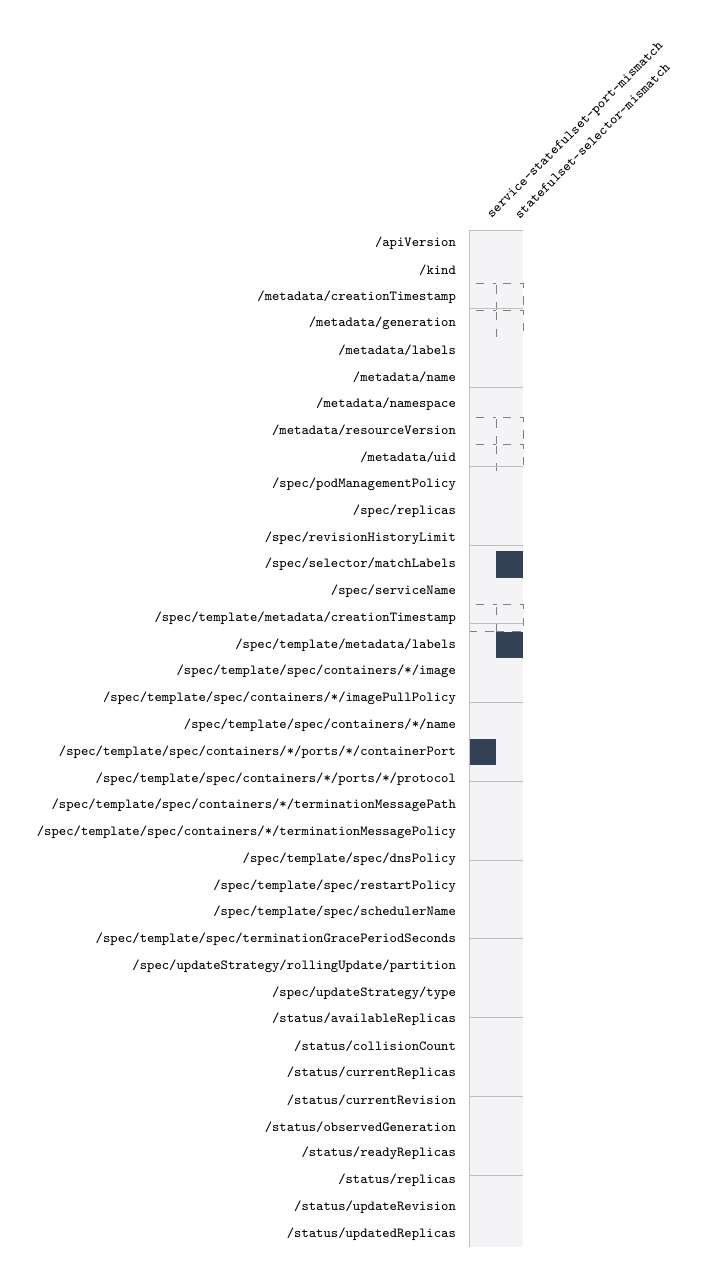
\begin{tikzpicture}[x=3.4mm,y=3.4mm]
\node[rotate=45,anchor=west,font=\ttfamily\tiny] at (0.5,0.25) {service-statefulset-port-mismatch};
\node[rotate=45,anchor=west,font=\ttfamily\tiny] at (1.5,0.25) {statefulset-selector-mismatch};
\node[anchor=east,font=\ttfamily\tiny] at (-0.15,-0.5) {/apiVersion};
\fill[fill={rgb,255:red,244;green,244;blue,246}] (0,-1) rectangle ++(1,1);
\fill[fill={rgb,255:red,244;green,244;blue,246}] (1,-1) rectangle ++(1,1);
\node[anchor=east,font=\ttfamily\tiny] at (-0.15,-1.5) {/kind};
\fill[fill={rgb,255:red,244;green,244;blue,246}] (0,-2) rectangle ++(1,1);
\fill[fill={rgb,255:red,244;green,244;blue,246}] (1,-2) rectangle ++(1,1);
\node[anchor=east,font=\ttfamily\tiny] at (-0.15,-2.5) {/metadata/creationTimestamp};
\fill[fill={rgb,255:red,244;green,244;blue,246}] (0,-3) rectangle ++(1,1);
\draw[gray,dashed,line width=0.2pt] (0,-3) rectangle ++(1,1);
\fill[fill={rgb,255:red,244;green,244;blue,246}] (1,-3) rectangle ++(1,1);
\draw[gray,dashed,line width=0.2pt] (1,-3) rectangle ++(1,1);
\node[anchor=east,font=\ttfamily\tiny] at (-0.15,-3.5) {/metadata/generation};
\fill[fill={rgb,255:red,244;green,244;blue,246}] (0,-4) rectangle ++(1,1);
\draw[gray,dashed,line width=0.2pt] (0,-4) rectangle ++(1,1);
\fill[fill={rgb,255:red,244;green,244;blue,246}] (1,-4) rectangle ++(1,1);
\draw[gray,dashed,line width=0.2pt] (1,-4) rectangle ++(1,1);
\node[anchor=east,font=\ttfamily\tiny] at (-0.15,-4.5) {/metadata/labels};
\fill[fill={rgb,255:red,244;green,244;blue,246}] (0,-5) rectangle ++(1,1);
\fill[fill={rgb,255:red,244;green,244;blue,246}] (1,-5) rectangle ++(1,1);
\node[anchor=east,font=\ttfamily\tiny] at (-0.15,-5.5) {/metadata/name};
\fill[fill={rgb,255:red,244;green,244;blue,246}] (0,-6) rectangle ++(1,1);
\fill[fill={rgb,255:red,244;green,244;blue,246}] (1,-6) rectangle ++(1,1);
\node[anchor=east,font=\ttfamily\tiny] at (-0.15,-6.5) {/metadata/namespace};
\fill[fill={rgb,255:red,244;green,244;blue,246}] (0,-7) rectangle ++(1,1);
\fill[fill={rgb,255:red,244;green,244;blue,246}] (1,-7) rectangle ++(1,1);
\node[anchor=east,font=\ttfamily\tiny] at (-0.15,-7.5) {/metadata/resourceVersion};
\fill[fill={rgb,255:red,244;green,244;blue,246}] (0,-8) rectangle ++(1,1);
\draw[gray,dashed,line width=0.2pt] (0,-8) rectangle ++(1,1);
\fill[fill={rgb,255:red,244;green,244;blue,246}] (1,-8) rectangle ++(1,1);
\draw[gray,dashed,line width=0.2pt] (1,-8) rectangle ++(1,1);
\node[anchor=east,font=\ttfamily\tiny] at (-0.15,-8.5) {/metadata/uid};
\fill[fill={rgb,255:red,244;green,244;blue,246}] (0,-9) rectangle ++(1,1);
\draw[gray,dashed,line width=0.2pt] (0,-9) rectangle ++(1,1);
\fill[fill={rgb,255:red,244;green,244;blue,246}] (1,-9) rectangle ++(1,1);
\draw[gray,dashed,line width=0.2pt] (1,-9) rectangle ++(1,1);
\node[anchor=east,font=\ttfamily\tiny] at (-0.15,-9.5) {/spec/podManagementPolicy};
\fill[fill={rgb,255:red,244;green,244;blue,246}] (0,-10) rectangle ++(1,1);
\fill[fill={rgb,255:red,244;green,244;blue,246}] (1,-10) rectangle ++(1,1);
\node[anchor=east,font=\ttfamily\tiny] at (-0.15,-10.5) {/spec/replicas};
\fill[fill={rgb,255:red,244;green,244;blue,246}] (0,-11) rectangle ++(1,1);
\fill[fill={rgb,255:red,244;green,244;blue,246}] (1,-11) rectangle ++(1,1);
\node[anchor=east,font=\ttfamily\tiny] at (-0.15,-11.5) {/spec/revisionHistoryLimit};
\fill[fill={rgb,255:red,244;green,244;blue,246}] (0,-12) rectangle ++(1,1);
\fill[fill={rgb,255:red,244;green,244;blue,246}] (1,-12) rectangle ++(1,1);
\node[anchor=east,font=\ttfamily\tiny] at (-0.15,-12.5) {/spec/selector/matchLabels};
\fill[fill={rgb,255:red,244;green,244;blue,246}] (0,-13) rectangle ++(1,1);
\fill[fill={rgb,255:red,51;green,65;blue,85}] (1,-13) rectangle ++(1,1);
\node[white,font=\tiny] at (1.5,-13.5) {$\ast$};
\node[anchor=east,font=\ttfamily\tiny] at (-0.15,-13.5) {/spec/serviceName};
\fill[fill={rgb,255:red,244;green,244;blue,246}] (0,-14) rectangle ++(1,1);
\fill[fill={rgb,255:red,244;green,244;blue,246}] (1,-14) rectangle ++(1,1);
\node[anchor=east,font=\ttfamily\tiny] at (-0.15,-14.5) {/spec/template/metadata/creationTimestamp};
\fill[fill={rgb,255:red,244;green,244;blue,246}] (0,-15) rectangle ++(1,1);
\draw[gray,dashed,line width=0.2pt] (0,-15) rectangle ++(1,1);
\fill[fill={rgb,255:red,244;green,244;blue,246}] (1,-15) rectangle ++(1,1);
\draw[gray,dashed,line width=0.2pt] (1,-15) rectangle ++(1,1);
\node[anchor=east,font=\ttfamily\tiny] at (-0.15,-15.5) {/spec/template/metadata/labels};
\fill[fill={rgb,255:red,244;green,244;blue,246}] (0,-16) rectangle ++(1,1);
\fill[fill={rgb,255:red,51;green,65;blue,85}] (1,-16) rectangle ++(1,1);
\node[white,font=\tiny] at (1.5,-16.5) {$\ast$};
\node[anchor=east,font=\ttfamily\tiny] at (-0.15,-16.5) {/spec/template/spec/containers/*/image};
\fill[fill={rgb,255:red,244;green,244;blue,246}] (0,-17) rectangle ++(1,1);
\fill[fill={rgb,255:red,244;green,244;blue,246}] (1,-17) rectangle ++(1,1);
\node[anchor=east,font=\ttfamily\tiny] at (-0.15,-17.5) {/spec/template/spec/containers/*/imagePullPolicy};
\fill[fill={rgb,255:red,244;green,244;blue,246}] (0,-18) rectangle ++(1,1);
\fill[fill={rgb,255:red,244;green,244;blue,246}] (1,-18) rectangle ++(1,1);
\node[anchor=east,font=\ttfamily\tiny] at (-0.15,-18.5) {/spec/template/spec/containers/*/name};
\fill[fill={rgb,255:red,244;green,244;blue,246}] (0,-19) rectangle ++(1,1);
\fill[fill={rgb,255:red,244;green,244;blue,246}] (1,-19) rectangle ++(1,1);
\node[anchor=east,font=\ttfamily\tiny] at (-0.15,-19.5) {/spec/template/spec/containers/*/ports/*/containerPort};
\fill[fill={rgb,255:red,51;green,65;blue,85}] (0,-20) rectangle ++(1,1);
\node[white,font=\tiny] at (0.5,-20.5) {$\ast$};
\fill[fill={rgb,255:red,244;green,244;blue,246}] (1,-20) rectangle ++(1,1);
\node[anchor=east,font=\ttfamily\tiny] at (-0.15,-20.5) {/spec/template/spec/containers/*/ports/*/protocol};
\fill[fill={rgb,255:red,244;green,244;blue,246}] (0,-21) rectangle ++(1,1);
\fill[fill={rgb,255:red,244;green,244;blue,246}] (1,-21) rectangle ++(1,1);
\node[anchor=east,font=\ttfamily\tiny] at (-0.15,-21.5) {/spec/template/spec/containers/*/terminationMessagePath};
\fill[fill={rgb,255:red,244;green,244;blue,246}] (0,-22) rectangle ++(1,1);
\fill[fill={rgb,255:red,244;green,244;blue,246}] (1,-22) rectangle ++(1,1);
\node[anchor=east,font=\ttfamily\tiny] at (-0.15,-22.5) {/spec/template/spec/containers/*/terminationMessagePolicy};
\fill[fill={rgb,255:red,244;green,244;blue,246}] (0,-23) rectangle ++(1,1);
\fill[fill={rgb,255:red,244;green,244;blue,246}] (1,-23) rectangle ++(1,1);
\node[anchor=east,font=\ttfamily\tiny] at (-0.15,-23.5) {/spec/template/spec/dnsPolicy};
\fill[fill={rgb,255:red,244;green,244;blue,246}] (0,-24) rectangle ++(1,1);
\fill[fill={rgb,255:red,244;green,244;blue,246}] (1,-24) rectangle ++(1,1);
\node[anchor=east,font=\ttfamily\tiny] at (-0.15,-24.5) {/spec/template/spec/restartPolicy};
\fill[fill={rgb,255:red,244;green,244;blue,246}] (0,-25) rectangle ++(1,1);
\fill[fill={rgb,255:red,244;green,244;blue,246}] (1,-25) rectangle ++(1,1);
\node[anchor=east,font=\ttfamily\tiny] at (-0.15,-25.5) {/spec/template/spec/schedulerName};
\fill[fill={rgb,255:red,244;green,244;blue,246}] (0,-26) rectangle ++(1,1);
\fill[fill={rgb,255:red,244;green,244;blue,246}] (1,-26) rectangle ++(1,1);
\node[anchor=east,font=\ttfamily\tiny] at (-0.15,-26.5) {/spec/template/spec/terminationGracePeriodSeconds};
\fill[fill={rgb,255:red,244;green,244;blue,246}] (0,-27) rectangle ++(1,1);
\fill[fill={rgb,255:red,244;green,244;blue,246}] (1,-27) rectangle ++(1,1);
\node[anchor=east,font=\ttfamily\tiny] at (-0.15,-27.5) {/spec/updateStrategy/rollingUpdate/partition};
\fill[fill={rgb,255:red,244;green,244;blue,246}] (0,-28) rectangle ++(1,1);
\fill[fill={rgb,255:red,244;green,244;blue,246}] (1,-28) rectangle ++(1,1);
\node[anchor=east,font=\ttfamily\tiny] at (-0.15,-28.5) {/spec/updateStrategy/type};
\fill[fill={rgb,255:red,244;green,244;blue,246}] (0,-29) rectangle ++(1,1);
\fill[fill={rgb,255:red,244;green,244;blue,246}] (1,-29) rectangle ++(1,1);
\node[anchor=east,font=\ttfamily\tiny] at (-0.15,-29.5) {/status/availableReplicas};
\fill[fill={rgb,255:red,244;green,244;blue,246}] (0,-30) rectangle ++(1,1);
\fill[fill={rgb,255:red,244;green,244;blue,246}] (1,-30) rectangle ++(1,1);
\node[anchor=east,font=\ttfamily\tiny] at (-0.15,-30.5) {/status/collisionCount};
\fill[fill={rgb,255:red,244;green,244;blue,246}] (0,-31) rectangle ++(1,1);
\fill[fill={rgb,255:red,244;green,244;blue,246}] (1,-31) rectangle ++(1,1);
\node[anchor=east,font=\ttfamily\tiny] at (-0.15,-31.5) {/status/currentReplicas};
\fill[fill={rgb,255:red,244;green,244;blue,246}] (0,-32) rectangle ++(1,1);
\fill[fill={rgb,255:red,244;green,244;blue,246}] (1,-32) rectangle ++(1,1);
\node[anchor=east,font=\ttfamily\tiny] at (-0.15,-32.5) {/status/currentRevision};
\fill[fill={rgb,255:red,244;green,244;blue,246}] (0,-33) rectangle ++(1,1);
\fill[fill={rgb,255:red,244;green,244;blue,246}] (1,-33) rectangle ++(1,1);
\node[anchor=east,font=\ttfamily\tiny] at (-0.15,-33.5) {/status/observedGeneration};
\fill[fill={rgb,255:red,244;green,244;blue,246}] (0,-34) rectangle ++(1,1);
\fill[fill={rgb,255:red,244;green,244;blue,246}] (1,-34) rectangle ++(1,1);
\node[anchor=east,font=\ttfamily\tiny] at (-0.15,-34.5) {/status/readyReplicas};
\fill[fill={rgb,255:red,244;green,244;blue,246}] (0,-35) rectangle ++(1,1);
\fill[fill={rgb,255:red,244;green,244;blue,246}] (1,-35) rectangle ++(1,1);
\node[anchor=east,font=\ttfamily\tiny] at (-0.15,-35.5) {/status/replicas};
\fill[fill={rgb,255:red,244;green,244;blue,246}] (0,-36) rectangle ++(1,1);
\fill[fill={rgb,255:red,244;green,244;blue,246}] (1,-36) rectangle ++(1,1);
\node[anchor=east,font=\ttfamily\tiny] at (-0.15,-36.5) {/status/updateRevision};
\fill[fill={rgb,255:red,244;green,244;blue,246}] (0,-37) rectangle ++(1,1);
\fill[fill={rgb,255:red,244;green,244;blue,246}] (1,-37) rectangle ++(1,1);
\node[anchor=east,font=\ttfamily\tiny] at (-0.15,-37.5) {/status/updatedReplicas};
\fill[fill={rgb,255:red,244;green,244;blue,246}] (0,-38) rectangle ++(1,1);
\fill[fill={rgb,255:red,244;green,244;blue,246}] (1,-38) rectangle ++(1,1);
\draw[gray!50,line width=0.2pt] (0,0) grid (2,-38);
\end{tikzpicture}

\par\medskip\noindent{\small\bfseries StorageClass}\par\smallskip
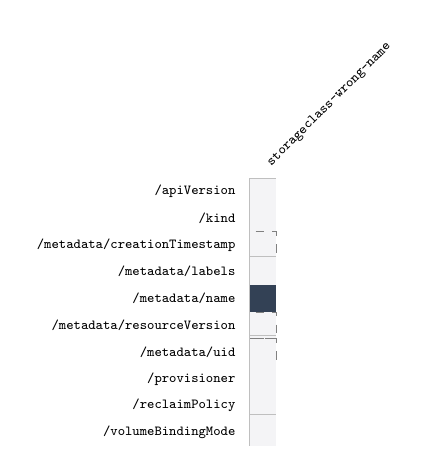
\begin{tikzpicture}[x=3.4mm,y=3.4mm]
\node[rotate=45,anchor=west,font=\ttfamily\tiny] at (0.5,0.25) {storageclass-wrong-name};
\node[anchor=east,font=\ttfamily\tiny] at (-0.15,-0.5) {/apiVersion};
\fill[fill={rgb,255:red,244;green,244;blue,246}] (0,-1) rectangle ++(1,1);
\node[anchor=east,font=\ttfamily\tiny] at (-0.15,-1.5) {/kind};
\fill[fill={rgb,255:red,244;green,244;blue,246}] (0,-2) rectangle ++(1,1);
\node[anchor=east,font=\ttfamily\tiny] at (-0.15,-2.5) {/metadata/creationTimestamp};
\fill[fill={rgb,255:red,244;green,244;blue,246}] (0,-3) rectangle ++(1,1);
\draw[gray,dashed,line width=0.2pt] (0,-3) rectangle ++(1,1);
\node[anchor=east,font=\ttfamily\tiny] at (-0.15,-3.5) {/metadata/labels};
\fill[fill={rgb,255:red,244;green,244;blue,246}] (0,-4) rectangle ++(1,1);
\node[anchor=east,font=\ttfamily\tiny] at (-0.15,-4.5) {/metadata/name};
\fill[fill={rgb,255:red,51;green,65;blue,85}] (0,-5) rectangle ++(1,1);
\node[white,font=\tiny] at (0.5,-5.5) {$\ast$};
\node[anchor=east,font=\ttfamily\tiny] at (-0.15,-5.5) {/metadata/resourceVersion};
\fill[fill={rgb,255:red,244;green,244;blue,246}] (0,-6) rectangle ++(1,1);
\draw[gray,dashed,line width=0.2pt] (0,-6) rectangle ++(1,1);
\node[anchor=east,font=\ttfamily\tiny] at (-0.15,-6.5) {/metadata/uid};
\fill[fill={rgb,255:red,244;green,244;blue,246}] (0,-7) rectangle ++(1,1);
\draw[gray,dashed,line width=0.2pt] (0,-7) rectangle ++(1,1);
\node[anchor=east,font=\ttfamily\tiny] at (-0.15,-7.5) {/provisioner};
\fill[fill={rgb,255:red,244;green,244;blue,246}] (0,-8) rectangle ++(1,1);
\node[anchor=east,font=\ttfamily\tiny] at (-0.15,-8.5) {/reclaimPolicy};
\fill[fill={rgb,255:red,244;green,244;blue,246}] (0,-9) rectangle ++(1,1);
\node[anchor=east,font=\ttfamily\tiny] at (-0.15,-9.5) {/volumeBindingMode};
\fill[fill={rgb,255:red,244;green,244;blue,246}] (0,-10) rectangle ++(1,1);
\draw[gray!50,line width=0.2pt] (0,0) grid (1,-10);
\end{tikzpicture}

\par\medskip\noindent{\small\bfseries VerticalPodAutoscaler}\par\smallskip
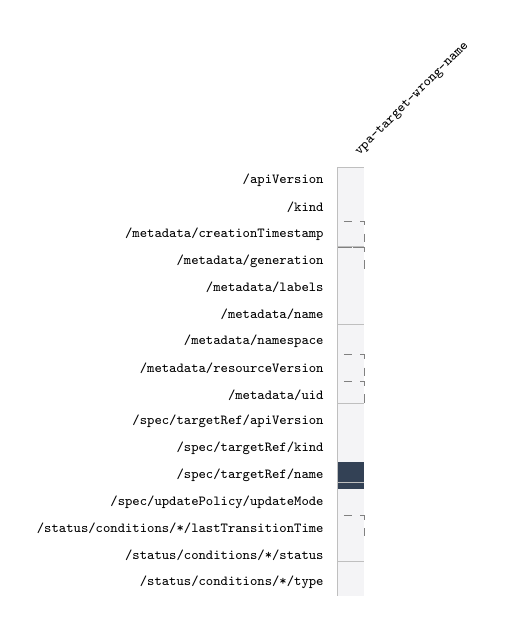
\begin{tikzpicture}[x=3.4mm,y=3.4mm]
\node[rotate=45,anchor=west,font=\ttfamily\tiny] at (0.5,0.25) {vpa-target-wrong-name};
\node[anchor=east,font=\ttfamily\tiny] at (-0.15,-0.5) {/apiVersion};
\fill[fill={rgb,255:red,244;green,244;blue,246}] (0,-1) rectangle ++(1,1);
\node[anchor=east,font=\ttfamily\tiny] at (-0.15,-1.5) {/kind};
\fill[fill={rgb,255:red,244;green,244;blue,246}] (0,-2) rectangle ++(1,1);
\node[anchor=east,font=\ttfamily\tiny] at (-0.15,-2.5) {/metadata/creationTimestamp};
\fill[fill={rgb,255:red,244;green,244;blue,246}] (0,-3) rectangle ++(1,1);
\draw[gray,dashed,line width=0.2pt] (0,-3) rectangle ++(1,1);
\node[anchor=east,font=\ttfamily\tiny] at (-0.15,-3.5) {/metadata/generation};
\fill[fill={rgb,255:red,244;green,244;blue,246}] (0,-4) rectangle ++(1,1);
\draw[gray,dashed,line width=0.2pt] (0,-4) rectangle ++(1,1);
\node[anchor=east,font=\ttfamily\tiny] at (-0.15,-4.5) {/metadata/labels};
\fill[fill={rgb,255:red,244;green,244;blue,246}] (0,-5) rectangle ++(1,1);
\node[anchor=east,font=\ttfamily\tiny] at (-0.15,-5.5) {/metadata/name};
\fill[fill={rgb,255:red,244;green,244;blue,246}] (0,-6) rectangle ++(1,1);
\node[anchor=east,font=\ttfamily\tiny] at (-0.15,-6.5) {/metadata/namespace};
\fill[fill={rgb,255:red,244;green,244;blue,246}] (0,-7) rectangle ++(1,1);
\node[anchor=east,font=\ttfamily\tiny] at (-0.15,-7.5) {/metadata/resourceVersion};
\fill[fill={rgb,255:red,244;green,244;blue,246}] (0,-8) rectangle ++(1,1);
\draw[gray,dashed,line width=0.2pt] (0,-8) rectangle ++(1,1);
\node[anchor=east,font=\ttfamily\tiny] at (-0.15,-8.5) {/metadata/uid};
\fill[fill={rgb,255:red,244;green,244;blue,246}] (0,-9) rectangle ++(1,1);
\draw[gray,dashed,line width=0.2pt] (0,-9) rectangle ++(1,1);
\node[anchor=east,font=\ttfamily\tiny] at (-0.15,-9.5) {/spec/targetRef/apiVersion};
\fill[fill={rgb,255:red,244;green,244;blue,246}] (0,-10) rectangle ++(1,1);
\node[anchor=east,font=\ttfamily\tiny] at (-0.15,-10.5) {/spec/targetRef/kind};
\fill[fill={rgb,255:red,244;green,244;blue,246}] (0,-11) rectangle ++(1,1);
\node[anchor=east,font=\ttfamily\tiny] at (-0.15,-11.5) {/spec/targetRef/name};
\fill[fill={rgb,255:red,51;green,65;blue,85}] (0,-12) rectangle ++(1,1);
\node[white,font=\tiny] at (0.5,-12.5) {$\ast$};
\node[anchor=east,font=\ttfamily\tiny] at (-0.15,-12.5) {/spec/updatePolicy/updateMode};
\fill[fill={rgb,255:red,244;green,244;blue,246}] (0,-13) rectangle ++(1,1);
\node[anchor=east,font=\ttfamily\tiny] at (-0.15,-13.5) {/status/conditions/*/lastTransitionTime};
\fill[fill={rgb,255:red,244;green,244;blue,246}] (0,-14) rectangle ++(1,1);
\draw[gray,dashed,line width=0.2pt] (0,-14) rectangle ++(1,1);
\node[anchor=east,font=\ttfamily\tiny] at (-0.15,-14.5) {/status/conditions/*/status};
\fill[fill={rgb,255:red,244;green,244;blue,246}] (0,-15) rectangle ++(1,1);
\node[anchor=east,font=\ttfamily\tiny] at (-0.15,-15.5) {/status/conditions/*/type};
\fill[fill={rgb,255:red,244;green,244;blue,246}] (0,-16) rectangle ++(1,1);
\draw[gray!50,line width=0.2pt] (0,0) grid (1,-16);
\end{tikzpicture}
